%% ut-thesis.tex -- document template for graduate theses at UofT
%%
%% Copyright (c) 1998-2012 Francois Pitt <fpitt@cs.utoronto.ca>
%% last updated at 09:43 (EDT) on Fri  1 Jun 2012
%%
%% This work may be distributed and/or modified under the conditions of
%% the LaTeX Project Public License, either version 1.3c of this license
%% or (at your option) any later version.
%% The latest version of this license is in
%%     http://www.latex-project.org/lppl.txt
%% and version 1.3c or later is part of all distributions of LaTeX
%% version 2005/12/01 or later.
%%
%% This work has the LPPL maintenance status "maintained".
%%
%% The Current Maintainer of this work is
%% Francois Pitt <fpitt@cs.utoronto.ca>.
%%
%% This work consists of the files listed in the accompanying README.

%% SUMMARY OF FEATURES:
%%
%% All environments, commands, and options provided by the `ut-thesis'
%% class will be described below, at the point where they should appear
%% in the document.  See the file `ut-thesis.cls' for more details.
%%
%% To explicitly set the pagestyle of any blank page inserted with
%% \cleardoublepage, use one of \clearemptydoublepage,
%% \clearplaindoublepage, \clearthesisdoublepage, or
%% \clearstandarddoublepage (to use the style currently in effect).
%%
%% For single-spaced quotes or quotations, use the `longquote' and
%% `longquotation' environments.


%%%%%%%%%%%%         PREAMBLE         %%%%%%%%%%%%

%%  - Default settings format a final copy (single-sided, normal
%%    margins, one-and-a-half-spaced with single-spaced notes).
%%  - For a rough copy (double-sided, normal margins, double-spaced,
%%    with the word "DRAFT" printed at each corner of every page), use
%%    the `draft' option.
%%  - The default global line spacing can be changed with one of the
%%    options `singlespaced', `onehalfspaced', or `doublespaced'.
%%  - Footnotes and marginal notes are all single-spaced by default, but
%%    can be made to have the same spacing as the rest of the document
%%    by using the option `standardspacednotes'.
%%  - The size of the margins can be changed with one of the options:
%%     . `narrowmargins' (1 1/4" left, 3/4" others),
%%     . `normalmargins' (1 1/4" left, 1" others),
%%     . `widemargins' (1 1/4" all),
%%     . `extrawidemargins' (1 1/2" all).
%%  - The pagestyle of "cleared" pages (empty pages inserted in
%%    two-sided documents to put the next page on the right-hand side)
%%    can be set with one of the options `cleardoublepagestyleempty',
%%    `cleardoublepagestyleplain', or `cleardoublepagestylestandard'.
%%  - Any other standard option for the `report' document class can be
%%    used to override the default or draft settings (such as `10pt',
%%    `11pt', `12pt'), and standard LaTeX packages can be used to
%%    further customize the layout and/or formatting of the document.

%% *** Add any desired options. ***
\documentclass[doublespaced]{ut-thesis}

%% *** Add \usepackage declarations here. ***
%% The standard packages `geometry' and `setspace' are already loaded by
%% `ut-thesis' -- see their documentation for details of the features
%% they provide.  In particular, you may use the \geometry command here
%% to adjust the margins if none of the ut-thesis options are suitable
%% (see the `geometry' package for details).  You may also use the
%% \setstretch command to set the line spacing to a value other than
%% single, one-and-a-half, or double spaced (see the `setspace' package
%% for details).
\usepackage{hyperref}
\usepackage{amsmath, amssymb, amsthm} % AMS packages
\usepackage{graphicx,color}           % Packages for graphics and color
\usepackage{pdfpages}
\usepackage{amsfonts}
%\usepackage[caption=false,font=footnotesize]{subfig}
\usepackage{caption}
\usepackage{subcaption}
\usepackage{algpseudocode}
\usepackage{algorithmicx}
\usepackage{algorithm}
\usepackage[titletoc]{appendix}
\usepackage{listings}
\usepackage{color}
\usepackage{csquotes}
\usepackage{quotchap}
%\usepackage{enumitem}
\usepackage{enumerate}


%\usepackage{tinycaptionfont}
%\usepackage{spconf}

% correct bad hyphenation here
%\hyphenation{op-tical net-works semi-conduc-tor}

%%%%%%%%%%%%%%%%%%%%%%%%%%%%%%%%%%%%%%%%%%%%%%%%%%%%%%%%%
%%%%%%%%%%%%%%%
%%                                                                    %%
%%                   ***   I M P O R T A N T   ***                    %%
%%                                                                    %%
%%  Fill in the following fields with the required information:       %%
%%   - \degree{...}       name of the degree obtained                 %%
%%   - \department{...}   name of the graduate department             %%
%%   - \gradyear{...}     year of graduation                          %%
%%   - \author{...}       name of the author                          %%
%%   - \title{...}        title of the thesis                         %%
%%%%%%%%%%%%%%%%%%%%%%%%%%%%%%%%%%%%%%%%%%%%%%%%%%%%%%%%%
%%%%%%%%%%%%%%%

%% *** Change this example to appropriate values. ***
\degree{Doctor of Philosophy}
\department{Electrical and Computer Engineering}
\gradyear{2016}
\author{Raymond Chun Hing Lo}
\title{Embodied Humanistic Intelligence: Design of Augmediated Reality Digital Eye Glass}

%% *** NOTE ***
%% Put here all other formatting commands that belong in the preamble.
%% In particular, you should put all of your \newcommand's,
%% \newenvironment's, \newtheorem's, etc. (in other words, all the
%% global definitions that you will need throughout your thesis) in a
%% separate file and use "\input{filename}" to input it here.


%% *** Adjust the following settings as desired. ***

%% List only down to subsections in the table of contents;
%% 0=chapter, 1=section, 2=subsection, 3=subsubsection, etc.
\setcounter{tocdepth}{2}

%% Make each page fill up the entire page.
\flushbottom


%%%%%%%%%%%%      MAIN  DOCUMENT      %%%%%%%%%%%%

\begin{document}
%\pagenumbering{roman}


%% This sets the page style and numbering for preliminary sections.
\begin{preliminary}

%% This generates the title page from the information given above.
\maketitle

%% There should be NOTHING between the title page and abstract.
%% However, if your document is two-sided and you want the abstract
%% _not_ to appear on the back of the title page, then uncomment the
%% following line.
%\cleardoublepage

%% This generates the abstract page, with the line spacing adjusted
%% according to SGS guidelines.
\begin{abstract}

%outline 

%Perhaps, it�s always been a dream for me and many of us to to acquire some sort of superhuman 
%capabilities. Fundamentally, humans are "bandwidth-limited" \cite{Rose:48}- that is, we can only process so much 
%information, see so far, and see so bright/dark. In the last hundreds of years, evolution has not made us much 
%stronger; however, innovation in technology has often offered us the possibility to acquire new capabilities and 
%transcend our own limitations.  For the past 10 years, I have dedicated my career to creating a new form of 
%computing that pushes our sensory capability, particularly with the human eye, and improves our everyday life 
%through augmented-reality (AR) digital eyeglasses. I argue that humans and machine shall not be treated as two 
%separate entities, but rather as one unified embodiment in the design of any wearable eyeglasses system. When 
%we start to design a machine that integrates human as a critical part of the feedback loop, we create a truly 
%humanistic intelligent computing platform that is intuitive to use and is limited only by our own imagination. 


%% *** Put your Abstract here. ***
%% (At most 150 words for M.Sc. or 350 words for Ph.D.)
%Humanistic Intelligence \cite{mann2001wearable}.
%
%Over the past 20 years, wearable computing has emerged as the perfect tool for embodying humanistic 
%intelligence (HI). HI is intelligence that arises when a human is part of the feedback loop of a computational process 
%in which the human and computer are inextricably intertwined. It is common in the field of human-computer 
%interaction to think of the human and computer as separate entities. (indeed, the term "HCI" emphasizes this 
%separateness by treating the human and computer as different entities that interact.) However, in HI theory, we 
%prefer not to think of the wearer and the computer with its associated I/O apparatus as separate entities. Instead, 
%we regard the computer as a second brain and its sensory modalities as additional senses, in which synthetic 
%synesthesia merges with the wearer's senses. When a wearable computer functions in a successful embodiment of 
%HI, the computer uses the human's mind and body as one of its peripherals, just as the human uses the computer 
%as a peripheral. This reciprocal relationship is at the heart of HI.

%portable, wearable...
%portable, notification, and on-demand
%wearable, always ready, and having human in the action
%example, digital eyeglasses, and 
%Observable
%

\end{abstract}
%% Anything placed between the abstract and table of contents will
%% appear on a separate page since the abstract ends with \newpage and
%% the table of contents starts with \clearpage.  Use \cleardoublepage
%% for anything that you want to appear on a right-hand page.

%% This generates a "dedication" section, if needed
%% (uncomment to have it appear in the document).
\begin{dedication}
%% *** Put your Dedication here. ***
Dedication Here
\end{dedication}

%% The `dedication' and `acknowledgements' sections do not create new
%% pages so if you want the two sections to appear on separate pages,
%% you should put an explicit \newpage between them.

%% This generates an "acknowledgements" section, if needed
%% (uncomment to have it appear in the document).
%\begin{acknowledgements}
%% *** Put your Acknowledgements here. ***
%\end{acknowledgements}

%% This generates the Table of Contents (on a separate page).
\tableofcontents

%% This generates the List of Tables (on a separate page), if needed
%% (uncomment to have it appear in the document).
%\listoftables

%% This generates the List of Figures (on a separate page), if needed
%% (uncomment to have it appear in the document).
%\listoffigures

%% You can add commands here to generate any other material that belongs
%% in the head matter (for example, List of Plates, Index of Symbols, or
%% List of Appendices).

%% End of the preliminary sections: reset page style and numbering.
\end{preliminary}


%%%%%%%%%%%%%%%%%%%%%%%%%%%%%%%%%%%%%%%%%%%%%%%%%%%%%%%%%
%%%%%%%%%%%%%%%
%%  Put your Chapters here; the easiest way to do this is to keep     %%
%%  each chapter in a separate file and `\include' all the files.     %%
%%  Each chapter file should start with "\chapter{ChapterName}".      %%
%%  Note that using `\include' instead of `\input' will make each     %%
%%  chapter start on a new page, and allow you to format only parts   %%
%%  of your thesis at a time by using `\includeonly'.                 %%
%%%%%%%%%%%%%%%%%%%%%%%%%%%%%%%%%%%%%%%%%%%%%%%%%%%%%%%%%
%%%%%%%%%%%%%%%

%% *** Include chapter files here. ***

\begin{savequote}[65mm]
%\begin{displayquote}
``Humanistic Intelligence [HI] is intelligence that arises because of a human being in the feedback 
loop of a computational process, where the human and computer are inextricably intertwined. When a 
wearable computer embodies HI and becomes so technologically advanced that its intelligence 
matches our own biological brain, something much more powerful emerges from this synergy that 
gives rise to superhuman intelligence within the single `cyborg' being."
%\end{displayquote}
\qauthor{-- Marvin Minsky, Ray Kurzweil, \\and Steve Mann~\cite{minsky2013society} }
\end{savequote}

\chapter{Introduction}
Fundamentally, human sensory capacity is ``bandwidth-limited". There are limits to how far humans can see, or how much information they can process~\cite{ophthalmology3rd}. We can only sense so much information and we can only detect a limited spectrum of light and sound~\cite{laming1986weber}. We can only process information at a limited rate~\cite{martin2009thermodynamics}.

To overcome these limitations, people have created many tools and 
inventions to revolutionize the way we ``see'' and understand our world. The first invention of 
eyeglasses -- a pair of plastic or glass lenses which had a specific prescription and was 
mounted in a frame that held them in front of a person's eyes -- was first documented in the 12th 
century~\cite{rosen1956invention} and was primarily used to correct for refractive errors. Today, 
specialized eyeglasses are also used for purposes such as magnifying an object of interest during a 
surgical procedure and protecting our eyes in more dangerous settings including welding or high-
power laser procedures. Modern advancements in technology, particularly in processing power and 
sensor capability, have allowed us to overcome our own limitations by enabling the creation of novel 
devices that can receive and process information much faster and in more versatile ways than humanly possible before. 
It is clear that such advancements have surpassed the pace of our own biological evolution. This 
dissertation presents the design of a digital form of eyeglass that can significantly improve our 
vision, extend our sensory capabilities, and create a new form of human computer interaction that is 
truly human-centric. 

\section{Introduction to `Digital' Eye Glass}
\label{introdigitalglass}

In the 1960s, Ivan Sutherland first described the concept of a head-mounted three dimensional 
display system which presented the user with a virtual, perspective-corrected, image that changes with 
respect to the user's head movement~\cite{sutherland1968head}. The apparatus, as shown in 
Fig.~\ref{ivanfullsetup}, was cumbersome and had to be mounted in the ceiling with a mechanical arm 
due to its weight and size. The display can only render a transparent ``wire frame" line drawing and no 
additional user inputs, such as hand gesture, can be provided. Most importantly, this concept was not 
ubiquitously adopted at the time because the rendered content did not provide information in a 
meaningful way with the real world. Also the information it provided had no direct connection with the real world (i.e. it was purely fictional, in the form of a cube rendered into space, but having nothing to do with that space). Despite all these shortcomings, this initial prototype inspired 
further research based on head-mounted systems for human-computer interaction 
~\cite{feiner1993knowledge,feiner1997touring,caudell1992augmented,stoakley1995virtual,billinghurst2015rapid,kato1999marker,billinghurst2002augmented}.


\begin{figure*}[t]
\centering
\begin{subfigure}[t]{1.75in}
  \centering
  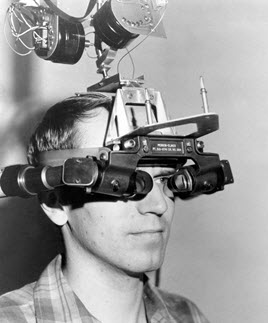
\includegraphics[height=2.0in]{ch1/figures/sutherland/3.jpeg}
  \caption{}
  \label{ivansetup1}
\end{subfigure}
\begin{subfigure}[t]{2.6in}
  \centering
  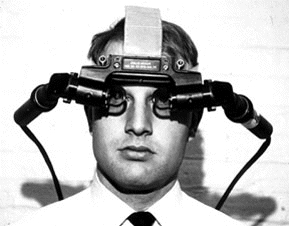
\includegraphics[height=2.0in]{ch1/figures/sutherland/2.jpeg}
  \caption{}
  \label{ivansetup2}
\end{subfigure}
\begin{subfigure}[t]{1.4in}
  \centering
  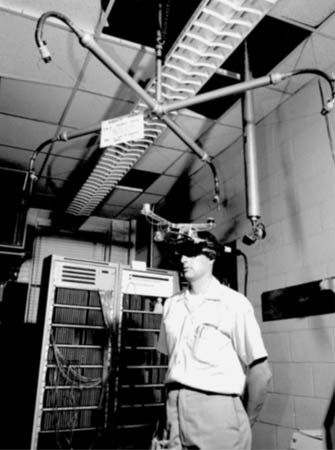
\includegraphics[height=2.0in]{ch1/figures/sutherland/1.jpeg}
  \caption{}
  \label{ivansetup3}
\end{subfigure}
\caption{(a) The head-mounted three dimensional display system, also known as ``The Sword of 
Damocles", worn by Donald L. Vickers, one of Ivan Sutherland's students~\cite{sutherland1968head}. (b) The head-mounted 
display and the optics with mini-CRT. A stereoscopic pair of computer-generated images were 
projected to the user's eyes through the half-silvered mirrors. The apparatus allows the user to see 
both the real world and virtual images at the same time and perform simple interaction with head 
motion~\cite{sutherland1968head}. (c) The mechanical, ultrasonic head position sensors, which were mounted in the ceiling and 
were designed at the MIT Lincoln Laboratory by Charles Seitz and Stylianos Pezaris, were used to 
retrieve the head position and orientation in real time~\cite{sutherland1968head}.  Shortcomings: (1) the material presented by this apparatus had no bearing on the real world, i.e. simply a wireframe cube, i.e. a fictional reality of sorts, and (2) the device was not a true wearable computer in the sense that it was a tethered desktop system.}
\label{ivanfullsetup}
\end{figure*}

\subsection{History of Wearable Computing}
In 1974, Mann invented the S.W.I.M. (Sequential Wave Imprinting Machine) which included a special kind of lock-in amplifier and wearable computer that could sweep for surveillance devices, and display the results of this "bug sweeping" activity on a linear array of sequentially illuminated light sources\cite{mann1992wavelets, impulse, mann2014sightfield, kineveillance}.  This system introduced the concept of "real reality" (phenomenological augmented reality) in contrast to virtual (fictional) reality of previous systems~\cite{mann2015par}.  Phenomenal/phenomenological augmented reality (PAR) is the reality of real physical phenomena/phenomenology such as sound waves, radio waves, veillance flux, etc., or other similar means of seeing beyond the usual visible spectrum.

In the 1980s, the idea of a Digital Eye Glass, Wearable Computer (WearComp) was introduced by 
Mann~\cite{mannaaai361, mann1994mediated, mannwyckofftr, aimone2003eyetap} as a 
practical realization of humanistic computing/humanistic intelligence (HI)~\cite{mann2001wearable, 
intelligentimageprocessing,presenceconnect,mann260}, and an extension of human capability for our 
everyday life. The WearComp project significantly transformed the way we think about wearable 
computers by proposing a framework for the integration of human into the signal processing path, 
thus creating the notion of humanistic intelligence~\cite{mann2001wearable, 
intelligentimageprocessing}. This work has important implications extending beyond the engineering 
challenges into the broader social implications, such as the concept of \emph{sousveillance}
~\cite{mann2002sousveillance, mann2004sousveillance, mann2006cyborglogging}) as opposed to 
the conventional notion of \emph{surveillance}, which emerge as a result of this new form of 
ubiquitous, wearable computing. 

\begin{figure}[htb]
\center
 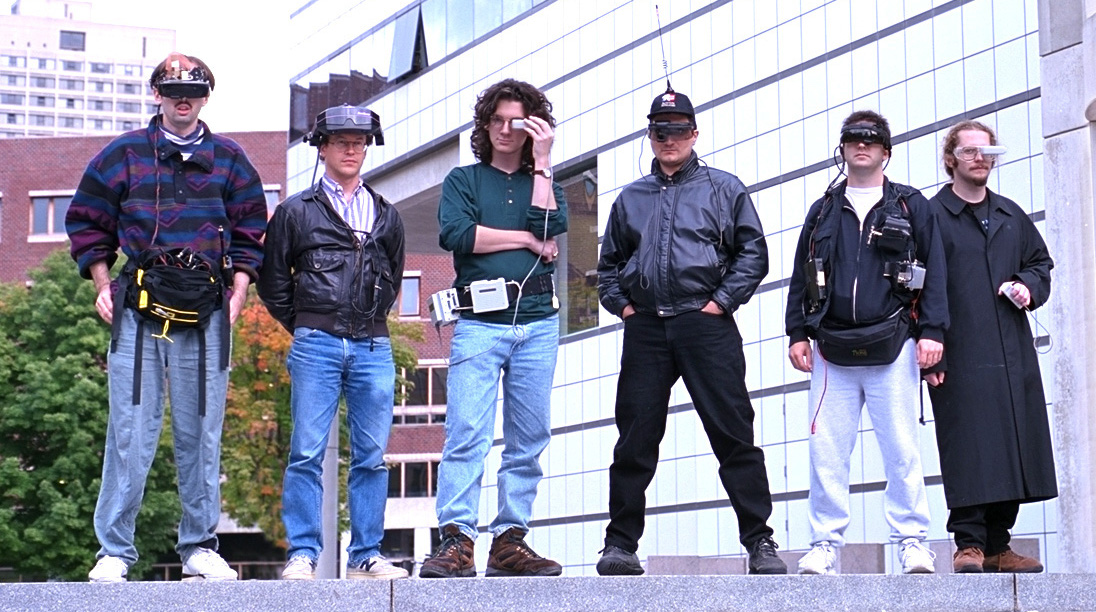
\includegraphics[width=5.5in]{ch1/figures/cyborgs.jpg}
 \caption{This picture shows the early members of the MIT wearable computing project founded (http://wearcam.org/nn.htm) by S. Mann (pictured leftmost) at MIT Media Lab. Particularly, individuals are pictured wearing computers which were connected wirelessly to create what Mann referred to as a 'safety net', an application which allows users to provide health and safety through sharing of sensory data streams~\cite{mann1997smart}. Image source: \url{http://www.wearcam.org/computing.html/imageinfo.html}. 
 }
 \label{fig:cyborgs}
\end{figure}

Subsequent to Mann's starting of the wearable computing project in the early 1990s, Thad Starner designed a wearable computer called ``The Lizzy'' based on the PC/104 form factor~\cite{starner1997augmented} in 1996. By continuously wearing computers in everyday life, a set of novel wearable applications such as``Augmented Memory"~\cite{starner1997augmented} which automatically augment based on the context of the user and augmented reality text-based applications, emerged.  Mann's wearable face recognizer~\cite{mann1996wearable} in 1996, and finger tracking~\cite{mann1997wearable}, was also built upon by others, where face detection and finger tracking~\cite{rhodes1997wearable} were emerged.

%Then Feiner\~cite{}

%Later in 1994, Mann then first transmitted images from his head-mounted camera system to the world wide web. See Figure~\ref{fig:mannglass} (c-d).

%These merging applications fundamentally require a better sensing technology, and algorithm to capture, to display with higher dynamic range display, and to process information around user's environment in real-time to provide a meaningful purpose for the uses.


\subsection{Digital Eye Glass}
%problem statement.
\begin{figure}[htb]
\center
 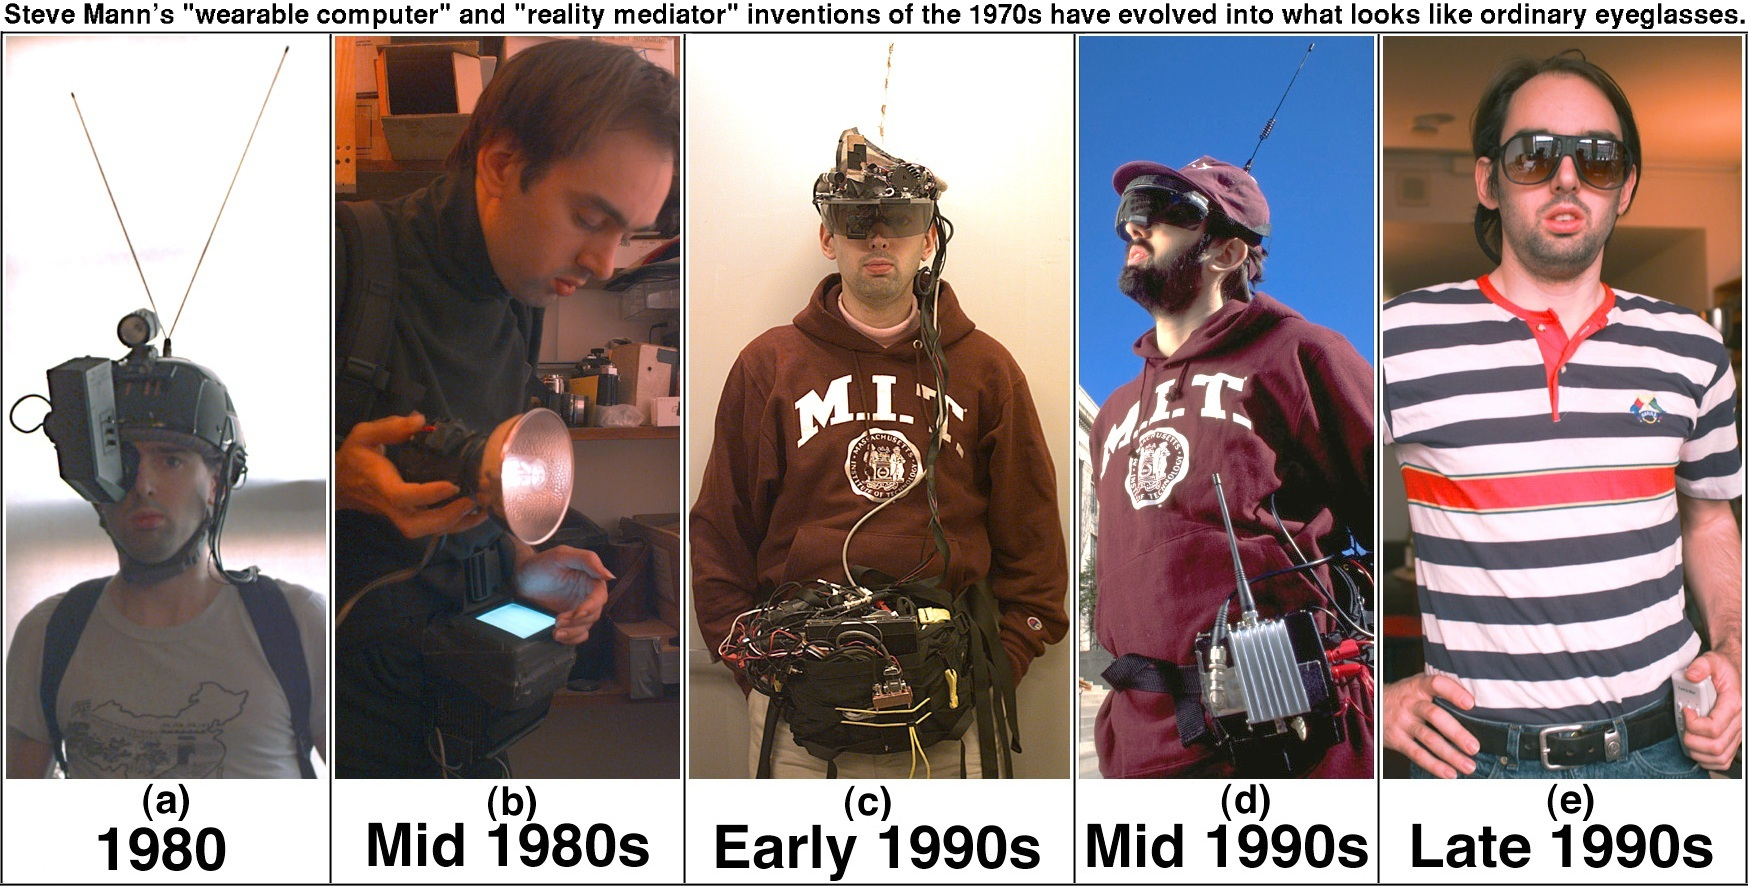
\includegraphics[width=5.5in]{ch1/figures/steve5.jpeg}
 \caption{(a) Mann's original wearable computer and phenomenological augmented reality system. The early prototype 
of the WearComp is a backpack-based computer system with a right eye display mounted on a 
helmet. Two radio wireless antennas run at different frequencies for full-duplex radio link for voice, 
video, and data communication~\cite{mann1994mediated}. (b) Prototypes of input devices with the WearComp 
project. An electronic flash light and a waist-mounted display are shown. (c-d) The world's first portable or 
wearable weblogging WearComp prototypes for Reality Mediator applications. The devices enable 
remote collaboration and the ability to alter the wearer's perception around the environment through 
Mediated Reality~\cite{mann1994mediated}. (e) A WearComp prototype which fits within the form 
factor of ordinary eyeglasses. Such a prototype is suitable for everyday usage in the society. The 
apparatus consists of a UNIX-based computer concealed under ordinary clothing, and a display and 
camera that fit within the eyeglasses~\cite{intelligentimageprocessing}.}
 \label{fig:mannglass}
\end{figure}

The EyeTap Digital Eye Glass functions as a seeing aid to help with specific tasks such as electric arc 
welding as well as in general day-to-day tasks, through a general-purpose computer in the form of 
eyeglasses or simply \emph{eye glass}~\cite{intelligentimageprocessing}. The EyeTap device causes 
the eye itself to, in effect, function as if it were both a camera and a display. Such a design gives the 
wearer the appearance of having a glass eye (See Fig.~\ref{fig:eyetap_mann_black}) so this 
phenomenon has become known as the ``Glass Eye'' effect~\cite{mann260}. 

\begin{figure}
  \center
  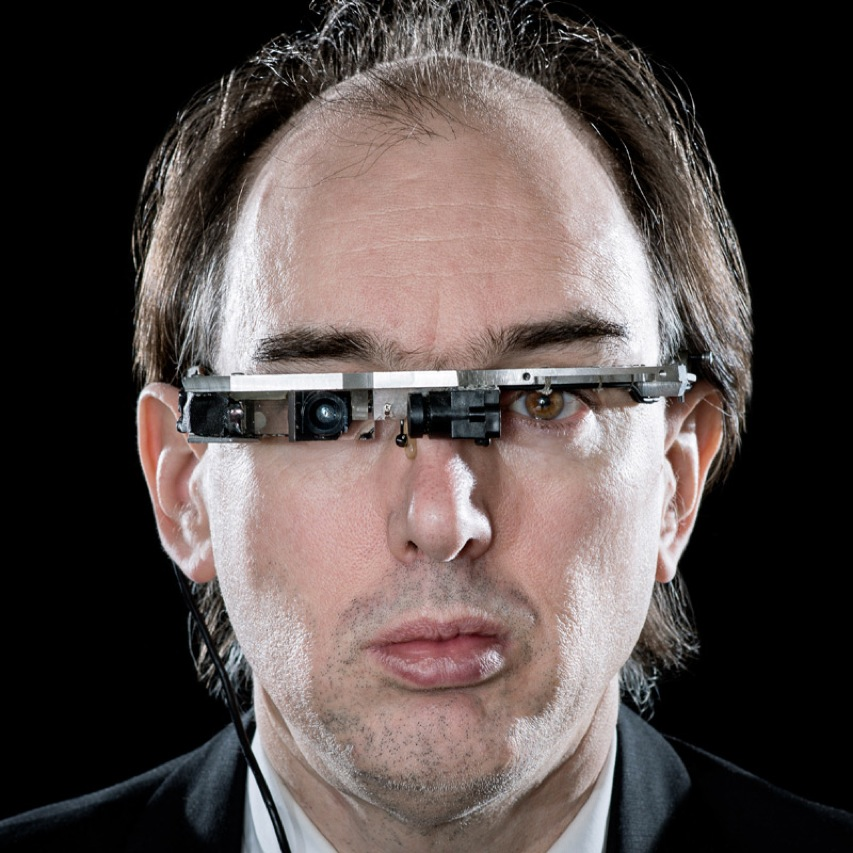
\includegraphics[width=3.0in]{ch1/figures/eyetap.jpg}
  \caption{The EyeTap system. The eye itself is, in effect, both the camera and display~\cite{mann2013steve}.}
  \label{fig:eyetap_mann_black}
\end{figure}

Thus EyeTap is sometimes called the ``Glass Eye'', as well as the ``Eye Glass'', or simply ``Glass''. 
Note the term ``Glass'' singular, rather than ``Glasses'' plural, has been widely used to describe this 
invention. Example applications running on the Glass included the Visual Memory 
Prosthetic~\cite{mannaaai361} which helps people, especially the elderly or those with visual 
impairment, to remember names, faces and other information in our environment. The EyeTap device 
can also service as a wayfinding tool with a GPS navigation system that goes beyond what is possible 
with traditional analog optical glasses. 

This apparatus helps the wearer see better in their everyday life, while also functioning as an interface 
for a general-purpose wearable computer. Today, companies such as Google are investing in the 
development of digital eyeglasses, such as Google Glass\footnote{\url{https://developers.google.com/
glass/}} that shares a number of features seen in the early EyeTap system. More recently, other 
companies such as Microsoft, Meta, and Intel have released various developer kits (e.g., 
Hololens\footnote{\url{https://www.microsoft.com/microsoft-hololens/en-us}} and Meta 
2\footnote{\url{https://www.metavision.com/}}) which provide a platform for the community to develop 
Aug-mediated Reality applications~\cite{mann1994mediated}.

Metaveillance/Metavision is the veillance of veillance (vision of vision), i.e. the sensing of sensors and the sensing of their capacity to sense. In the same way that a meta-conversation is a conversation about conversations, meta data is data about data, etc., metavision is the vision of vision. Metaveillance/metavision, when combined with abakography, results in a phenomenological augmented reality that makes real-world physical phenomena visible~\cite{toposculpting_ccece2014}.

Mann's metaveillance apparatus evolved toward a general-purpose wearable computer with wearable camera and display, equipped with gesture-sensing capabilities, so that it responds to the wearer's own self-gestures (e.g. it can see the wearer's own hands and thus create an interactional space in which the main design tools that the user uses are his or her own hands)~\cite{mannieeecomputer}. Mann's coined the term "Synthetic Synesthesia of the Sixth Sense", often abbreviated "SixthSense", to describe these gesture-based wearable computer systems~\cite{cyborg, geary2002body}.

Mann, Huang, Janzen, Lo, and others, added 3D depth-sensing capability to Sixth Sense in 2010, and used the Sixth Sense system to assist the blind and visually impaired~\cite{mann2011blind}.

In 2012, Mann and Gribetz joined forces in a collaboration that combined Mann's Sixth Sense and Metaveillance/Metavision technologies toward the production of a commercial product (patent written in 2012 and filed on January 3, 2013~\cite{patentmetadepth}).

By further adding the Toposculpting invention, a combination of three important technologies resulted:
1. Sixth Sense;
2. Metaveillance/Metavision;
3. Toposcuplting (topological sculpting), i.e. using 3D gesture-recognition for computational lightpainting by way of wearable computational photography for abakographic user-interfaces~\cite{patentmetabakography}. Subsequently, Gribetz (CEO), Mann (Chief Scientist), and Lo (Chief Technology Officer) joined forces to found the new company Meta Company, and introduce to the world the concept of Extramissive Spatial Imaging Glass~\cite{gribetz2014extramissive}. 

\section{A Theory of Glass: Background information}
%{\bf Note to reviewers:}
%{\em This section presents a review of Generations 1-4 of Digital Eye Glass.
%This section appears in another paper submission to i-Society 2013.
%If both papers are accepted for publication, the overlap will be
%eliminated to avoid double-publishing of this section.}

Digital Eye Glass is a wearable computer system that reconfigures the eye(s)
for Aug-mediated Reality, i.e. a visual reality that can be augmented or
deliberately diminished to, for example, help people see better by enhancing the image through 
magnification or contrast improvement in their everyday life through a `visual 
filter'~\cite{mann1994mediated}. 
In this sense, EyeTap was originally referred to as ``Glass'' rather than ``Glasses'' (the more common plural 
form of the word), as shown in Fig.~\ref{fig:glass} (the ``glass eye'' effect). 

\begin{figure}
\center
  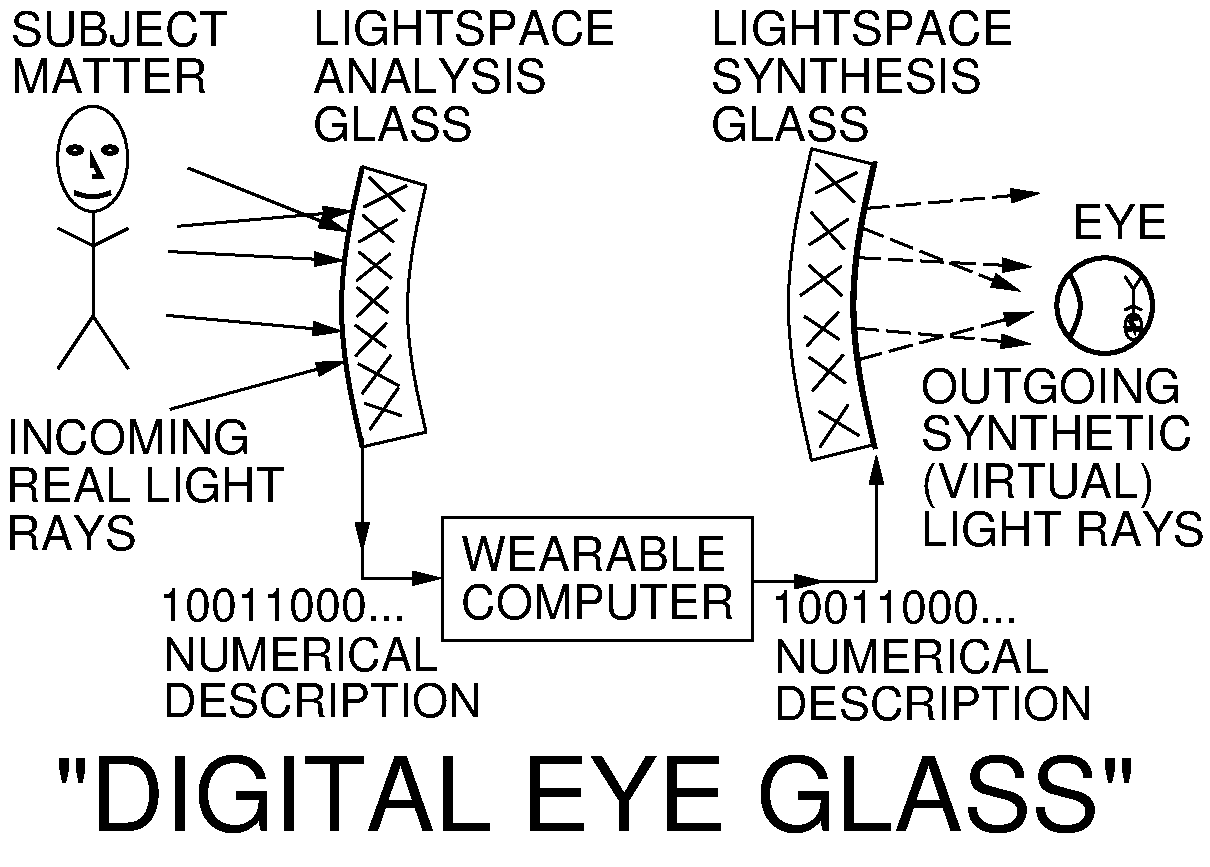
\includegraphics[width=3.5in]{ch6/figs/Glass.pdf}
  \caption{A theory of Glass: rays of eyeward bound light are captured
           by an ``analysis glass'', then processed by the wearable computer
           in the glass system, and then re-synthesized by a
           ``synthesis glass''~\cite{mann2013freeglass}.}
  \label{fig:glass}
\end{figure}

Rays of eyeward-bound light strike a ``Lightspace Analysis Glass'' (which need not necessarily be flat, 
and is therefore depicted as being curved), are converted to numbers which may then be processed 
by the wearable computer. The resulting numbers are fed to a ``Lightspace Synthesis Glass'' to be 
converted back into light.  This allows the wearable computer to become a visual intermediary, to, for 
example, diminish the bright areas
of the Subject Matter, and Augment/Mediate the bright areas, before resynthesizing the rays of light 
into the Eye, as shown in Fig~\ref{fig:glass}.

\subsection{Generation-1 Glass:}
The original approximation prototype of this glass was built in 1978, using a television camera as the 
``Lightspace Analysis Glass'' a miniature glass cathode-ray tube display as the ``Lightspace Synthesis 
Glass'' (over the right eye), and some electric circuits as the wearable computer, as shown in 
Fig.~\ref{fig:mannglass} (a).

Because the camera was located beside the eye, the long-term effects after many hours of wearing 
the apparatus consisted of an adaptation to this strange way of seeing, and the adaptation persisted 
after the removal of the apparatus~\cite{mann1994mediated}. 

Others found similar effects. For example, George Stratton in his work of 1896, with an upside-down 
glass
(done optically rather than electrically), found that it took him about a week to adapt to seeing with 
mediated vision, and about one full day to return to seeing properly (normally) after removing the 
glass~\cite{stratton1897vision}.

It was observed that mappings that deviate moderately from what the unaided eye saw, were harder to 
``forget'' than mappings that were either closer to or further from what the unaided eye saw.  The 
camera must, in effect be the eye itself, if we were to avoid the strange ``flashback'' effects and other 
fatigues due to accommodation to the Generation-1 Glass~\cite{schor1987fatigue}.

\begin{figure}
  \center
  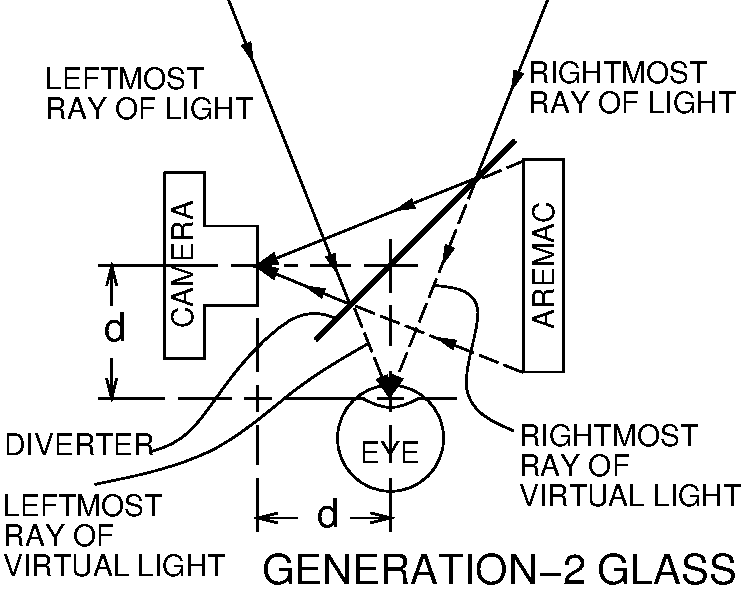
\includegraphics[width=3.5in]{ch6/figs/GlassGen2.pdf}
  \caption{Generation-2 Glass: The eye itself is, in effect, both the camera
           and display.  This eliminates the undesirable ``flashback'' effects
           that otherwise arise from long-term usage~\cite{mann2013freeglass}.}
  \label{fig:gentwo}
\end{figure}

\subsection{Generation-2 Glass}
Generation-2 Glass is developed in which Rays of eyeward-bound light were diverted into a camera 
system that feeds to the wearable computer which then drives an Lightspace Synthesis 
Glass~\cite{mann2001aremac}). In this way, rays of light that would have entered the unaided eye are 
collinear with rays of light presented by the Gen-2 Glass (Fig~\ref{fig:gentwo}). This setup addressed 
the ``flashback'' effects in Gen-1 Glass by carefully aligning the real-world and mediated content. 
However, it does not provide any real world tracking or refocusing capability, and assumes that the 
user is looking into the far range only.

\subsection{Generation-3 Glass}
Particularly in monocular systems, when one eye is focused on a display, and the other is focused on 
direct
``reality'', there is a difference in focal distance between the two eyes. To overcome this problem, 
Generation-3 Glass was developed using a special display called an 
``aremac''~\cite{mann2001aremac} which has the ability to present visual information at an apparent 
focal distance that can be controlled by the wearable computer. The computer senses where objects 
are in 3-dimensional space, and makes an inference as to what range of focal distances the non-
glass-eye can focus to. Information is presented to the glass-eye in this same focal range, which is 
automatically updated several times per second.

\begin{figure}
  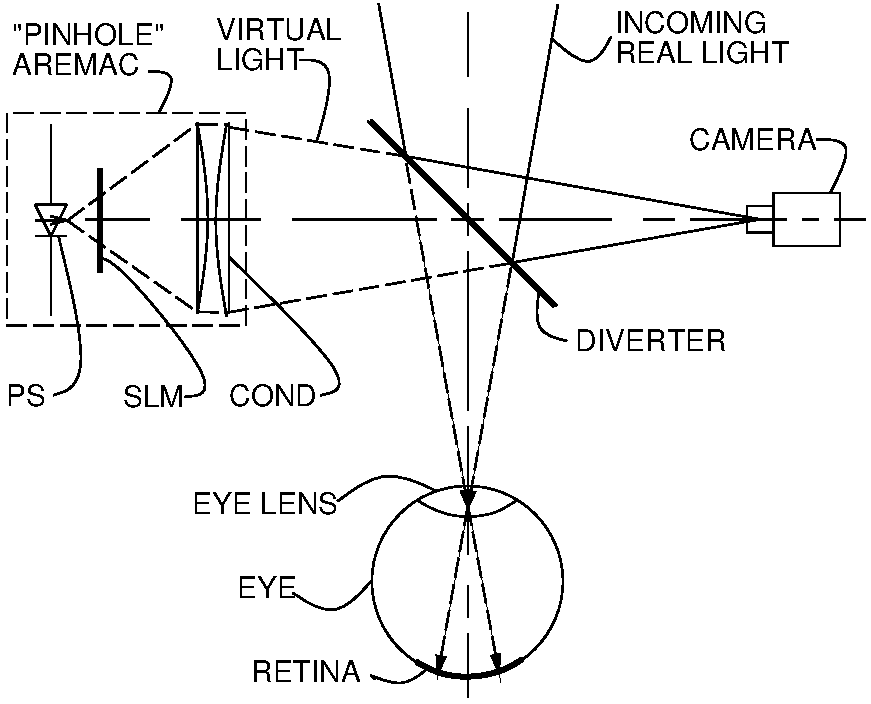
\includegraphics[height=2.4in]{ch6/figs/GlassGen4a.pdf}
  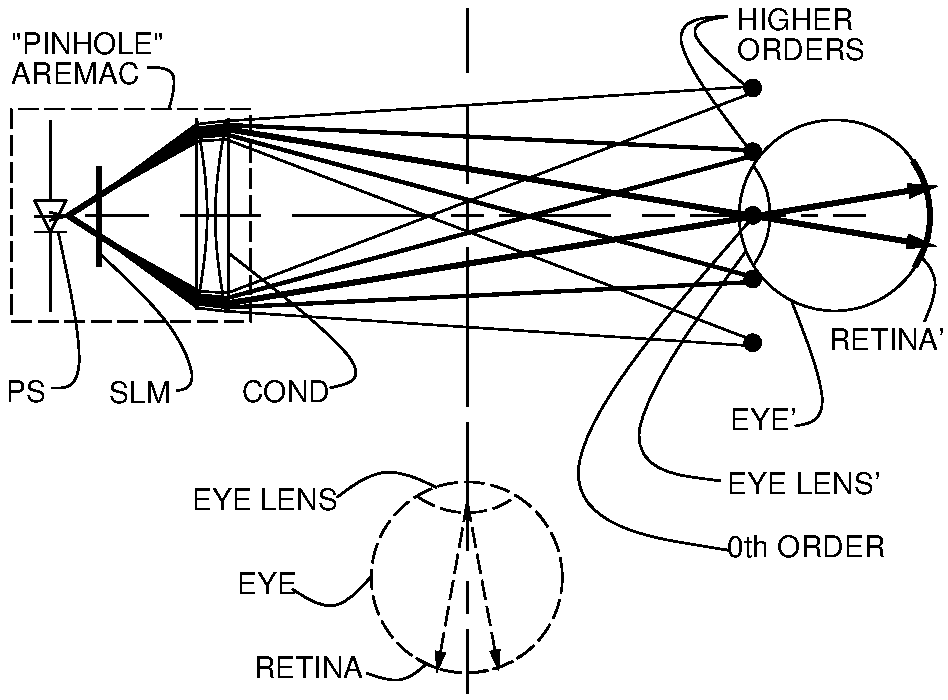
\includegraphics[height=2.4in]{ch6/figs/GlassGen4b.pdf}\\
  {\sffamily \large GENERATION-4 GLASS}\\
  \caption{Generation-4 Glass uses a laser light source to achieve
           infinite depth-of-focus to bypass the eye's lens.  Therefore,
           the glass-eye is not presented with information at any particular
           focal distance, leaving it free to focus at whatever distance the
           other eye is focused to~\cite{mann2013freeglass}.}
  \label{fig:genfour}
\end{figure}

\subsection{Generation-4 Glass}
While looking at objects in various focal planes, such as looking at a distant object through a nearby 
screen or chainlink fence, some problems remained with the Generation-3 Glass. Often, this may 
create eye fatigue due to the accommodation and vergence issue~\cite{hoffman2008vergence}. 

These problems were overcome with the Generation-4 Glass.  The Gen-4 Glass uses a laser light 
source
with a spatial light modulator, and related apparatus, to attain an infinite depth-of-focus, so that the 
displayed information is always in focus regardless of where the eye focuses. The laser EyeTap 
bypasses the lens of the glass-eye and forms an image directly on the retina. In this way, the Gen-4 
Glass does not cause the eye to focus at any particular distance, leaving it free to focus where the 
non-glass eye is focused (Fig~\ref{fig:genfour}).

Generations~2 to~4 Glass were known as ``EyeTap Digital Eye Glass''~\cite{edeg} (the word ``Glass'' 
appears in its singular form, not plural, i.e., ``Eye Glass'' not ``Eye Glasses'').

The result was a natural experience with zero eye strain and could be worn continuously many hours 
a day for many years. The Generation-4 Glass prototype was presented in 1999 and described in 
detail in 2001~\cite{intelligentimageprocessing} (Fig.~\ref{fig:mann_glass_google} (leftmost)).
% (the cover, first page, and pages 31-32) of Abilities Magazine, Issue 69, Winter 2006.

\begin{figure}
  \centering
  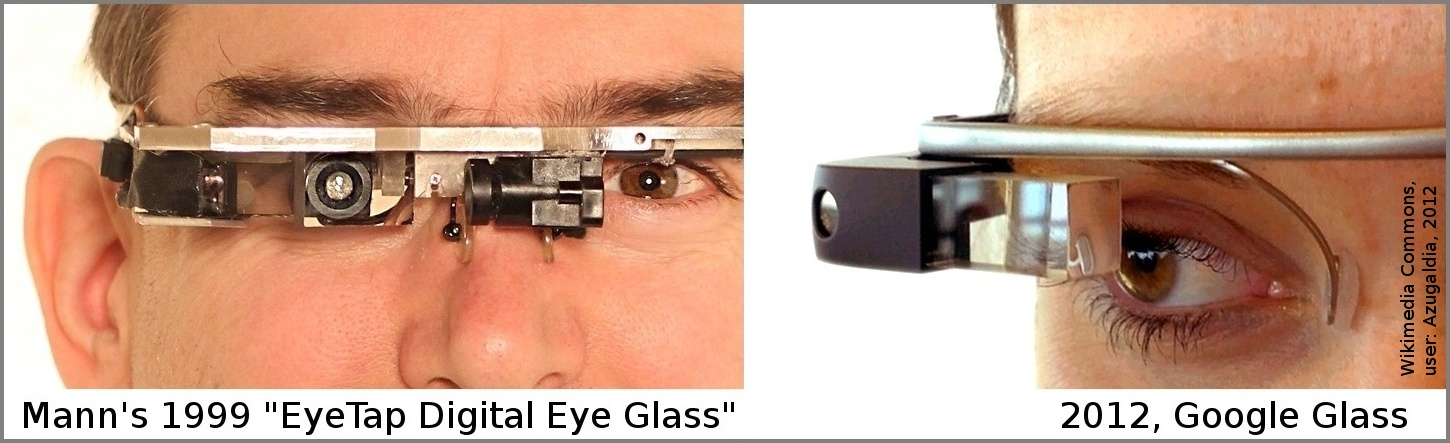
\includegraphics[width=5.5in]{ch6/figs/MannGlass_GoogleGlass_with_narrowborder_closer.jpg}\\
  \caption{Leftmost: Generation-4 Glass completed in 1999.
         {\bf The eye itself is the camera exactly!}
         That is why the ``Digital Eye Glass'' is also known as
         the ``GlassEye'' (The eye looks exactly like a camera lens).  This
         eliminates long-term dizziness, vertigo, and flashback effects
         that can otherwise persist long after the Glass is removed.
         Rightmost: Google Glass, 2012, where the camera being positioned to one
         side of the eye makes it a Generation-1 Glass, subject to some
         of the problems discovered earlier on ~\protect\cite{mann2013vision,mann2013freeglass}.
        }
  \label{fig:mann_glass_google}
\end{figure}

\subsection{Generation-5 Glass}
To further expand on the earlier work, Generation-5 is defined as being bi-directional in its light sensing 
and light output capabilities.  In this way, the Gen-5 Glass senses both the scene in front of the wearer 
as well as the wearer's
own eyes; it also illuminates both the wearer's eyes and the scene in front of the wearer 
(Fig~\ref{fig:genfive})

%\begin{figure}
\begin{figure}
  \centering
  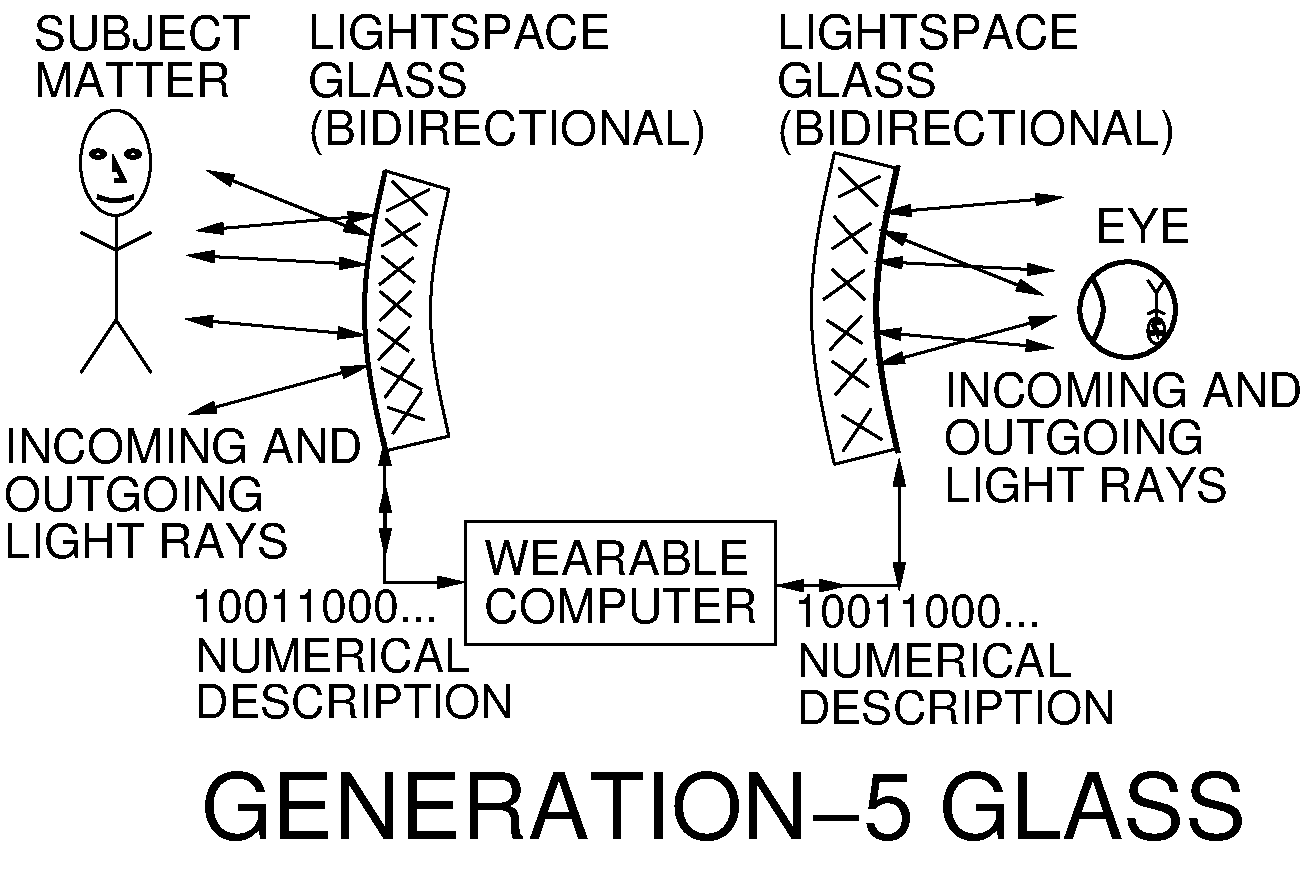
\includegraphics[width=3.75in]{ch6/figs/GL455.pdf}\\
  \caption{Proposed Generation-5 Glass.  Conceptually it is characterized
           by a bi-directional sensing and display modality.  Rays of light
           are sensed from BOTH THE SCENE AND THE EYE.  This facilitates
           eye-tracking as well as scene analysis. Computer-generated rays of light are also sent to 
BOTH THE
           EYE AND THE SCENE to facilitate active vision as well as
           being able to display content to other people who are not wearing
           the glass~\cite{mann2013freeglass}.}
  \label{fig:genfive}
\end{figure}

The development of the Gen-5 Glass is the focus of this thesis, which aims to create a ubiquitous 
wearable computing platform that enables a truly human-centric, intuitive computing environment by 
providing seamless integration between the human and the computer.

The Gen-5 Glass computing platform consists of two major components:
\begin{itemize}
  \item a hardware arrangement that consists of true stereoscopic 3D display glass and a time-of-flight 
3D range-sensing camera.  Other accessory devices such as a
        miniature laser data projector, eye-tracker, inertia measurement units (IMU), and brain-computer 
interface   sensors are also attached;
  \item a sophisticated software environment that simulates the EyeTap
        principle.  Because the camera is a 3D camera, it captures spatial-tonal
        information, allowing its point-of-view to be re-rendered from a
        left Point-of-Eye for the left eye, and, separately, a
        right Point-of-Eye for the right eye of the wearer.
\end{itemize}

A number of technical challenges arose in the creation of the Gen-5 Digital Eye Glass system, 
including optics design, calibration and alignment, head tracking and gesture tracking, form factor, 
latency management, human-computer interaction techniques, and Humanistic Intelligence 
(HI)~\cite{azuma1997survey, azuma2001recent, mann2001wearable}  which has recently become an 
active area of research. Specifically, the Humanistic Intelligence (HI) 
Framework~\cite{mann2001wearable} brings forth various topics in design decision and a new form of 
intelligent signal processing which forms an important basis of this thesis. One profound aspect of HI 
is the understanding of how human (and the human brain) should be an integral part of the computer 
system to create the superhuman intelligence as shown in Fig.~\ref{fig:hiflow}. The creation of the 
synergy between human and computer, which is summarized in the quote by Kurzweil, Minsky, and 
Mann~\cite{minsky2013society} at the beginning of the chapter, has a significant implication on the 
future of wearable computing. In the following section, a detailed description of the HI theories, as well 
as the core focus of the thesis in extending human capabilities, will be described.

\section{Humanistic Intelligence Framework}
\label{hiframeworks}

Many of the inventions and advancements in technology have changed the way we communicate and 
how we interact with the world. For example, the ability to communicate wirelessly with a handheld 
device (such as a mobile phone) radically changed the way we share and exchange information in 
this society. Trillions of instant messages are being sent per year\footnote{Mobile message traffic 
worldwide in 2012 and 2017 (in trillions)~\url{https://www.statista.com/statistics/262005/mobile-
message-traffic-worldwide/}} and billions of images are being uploaded and shared across the world 
daily\footnote{Internet Trends 2016 - Code Conference~\url{http://www.kpcb.com/internet-trends}}. 
Meanwhile, the recent innovation in human-computer interfaces from multi-touch interfaces to 
augmented, virtual, mixed, or aug-mediated reality interfaces have further redefined how we interact 
with the real world and the digital world. Computers are becoming increasingly more capable as they 
are equipped with more sensors such as motion sensors, depth sensors, or biometric sensors, which 
allow computers to observe human and infer our behaviours in our everyday lives and to act as our 
``personal assistant". Inevitably, the future of wearable computing will be characterized by an 
extremely close synergy between humans and computers. A set of questions and research problems 
arise as computers and humans are no longer separate entities in the feedback loop, and these 
questions lead to the field of research in Humanistic Intelligence (HI). 

\begin{figure}[htb]
\center
 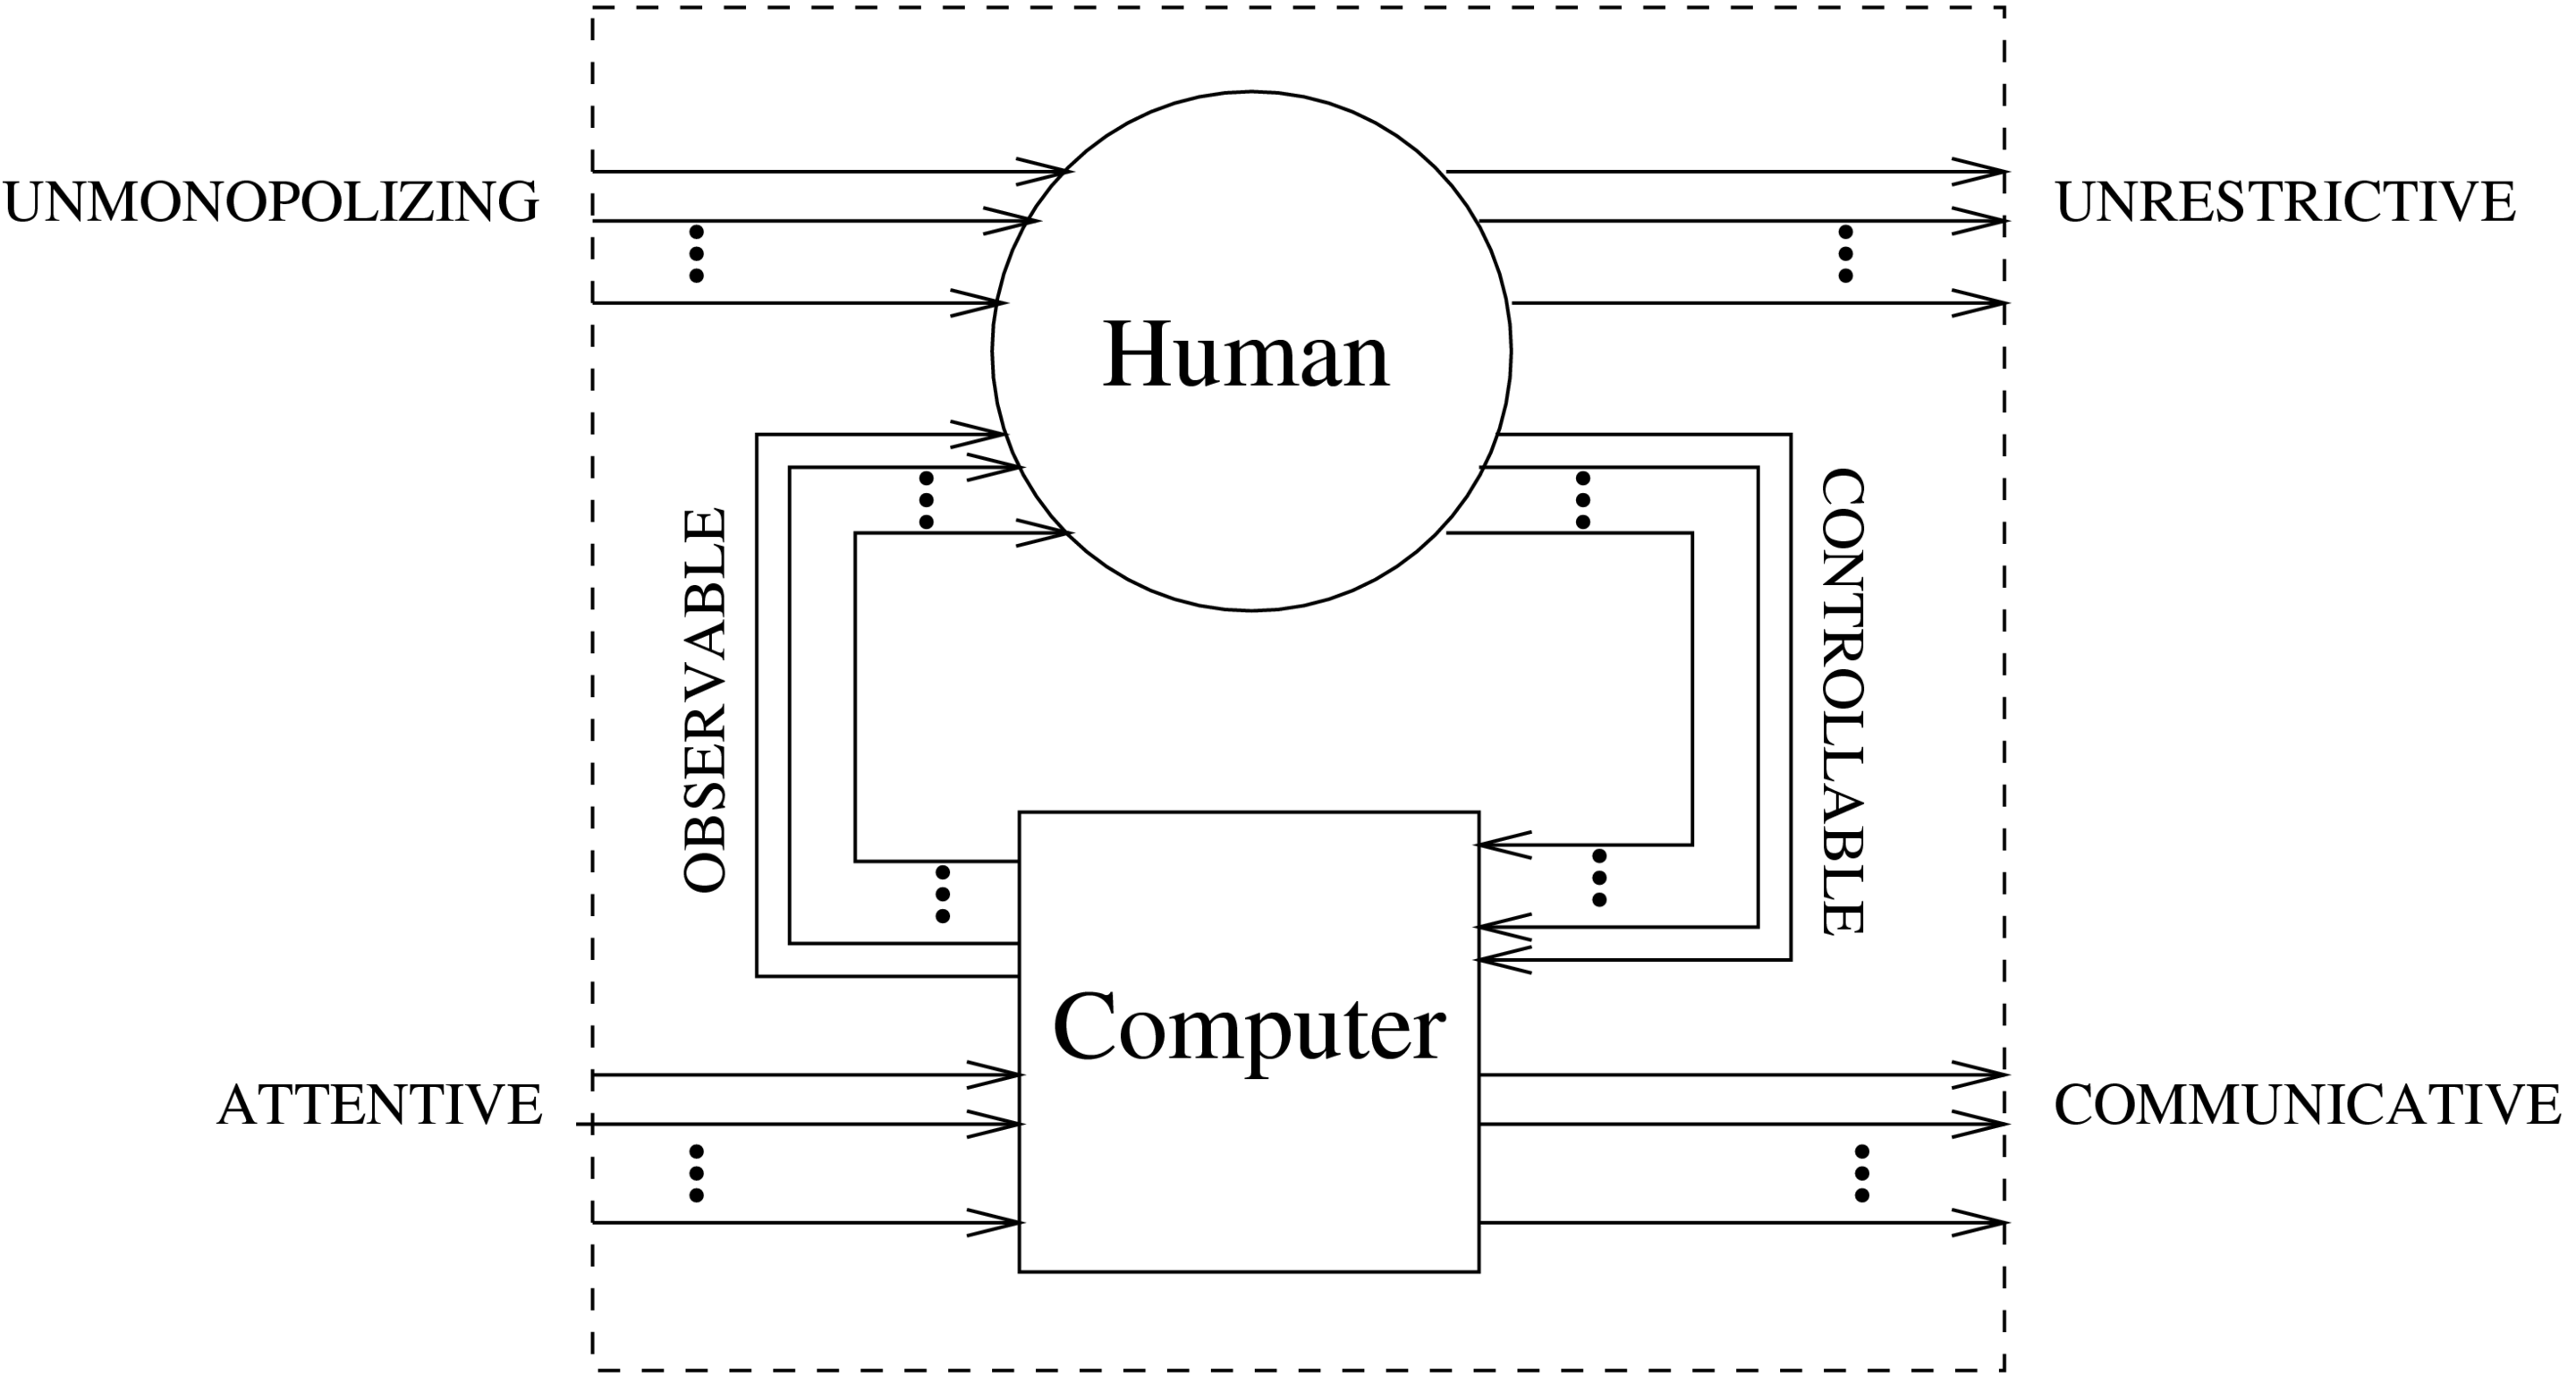
\includegraphics[width=6.0in]{ch1/figures/Humanistic_intelligence_wearcompdef_multichannel6only.png}
 \caption{The six signal flow paths in the Humanistic Intelligence Framework. These six signal flow paths 
each define one of the six attributes of WearComp~\cite{mann2001wearable}.}
 \label{fig:hiflow}
\end{figure}

One important aspect of HI is characterized by the processing hardware that is inextricably intertwined 
with a human being to function as a true extension of the user's mind and body. That is, the hardware 
is constant (`always ready'), provides augmentation (computing is NOT the primary task), and 
mediation (encapsulates the user). The notation of mediation is to create the ability to manage the 
information flow from the outside world, which creates a strong user empowerment tool.

The six basic signal flow paths of WearComp can be briefly summarized as follows 
(Fig.~\ref{fig:hiflow}): 

%REWRITE THIS SHIT....
\begin{enumerate}
   \item Unmonopolizing 
   \begin{itemize}
     \item The hardware does not isolate one from the outside world (e.g., replace the reality with a 
virtual world). Ideally, the WearComp device provides enhanced sensory capabilities. It may, however, 
facilitate mediation (augmenting, altering, or deliberately diminishing) of these sensory capabilities.  
   \end{itemize}
   \item Attentive
   \begin{itemize}
     \item The hardware has awareness of the environment with multi-modal and multi-sensory inputs. 
For example, one may want to combine a depth sensing camera, color camera, and perhaps fish eye 
camera to the system, and this ultimately gives the user increased situational awareness.
   \end{itemize}
   \item Unrestrictive
   \begin{itemize}
     \item The hardware is mobile and allows the user to perform other everyday tasks, e.g., one can 
give inputs to the system while walking down stairs or jogging without being restricted by the wearable 
system.
   \end{itemize}
   \item Communicative
   \begin{itemize}
     \item The hardware is used as a communication medium, as a means of assisting the user with the 
production of expressive or communicative media.
   \end{itemize}
   \item Observable
   \begin{itemize}
     \item The hardware provides user feedback continuously and is always observable within some 
reasonable limitations (e.g., the computer screen is not visible during the blinking of the eye).
   \end{itemize}
   \item Controllable
   \begin{itemize}
     \item The hardware is responsive and the user can take control over any part of the system when 
necessary. Any automated process and control loop shall include manual override control at any 
moment. 
   \end{itemize}
\end{enumerate}


Among these criteria, the key limiting factor in the realization of aug-mediated reality is that the 
experience enabled by the system can only be as good as the components used to create it. The 
limited dynamic range of the sensors, in particular, had hindered the Digital Eye Glass to be 
ubiquitously adopted in many situations. The lack of dynamic range of the sensor creates many ``blind 
spots'' or failure modes in a real world scene where the user and the computer may fail to see clearly. 
Thus, one key objective of this thesis is to address these shortcomings, and provide a real-time 
solution which pushes the boundary of the research on high dynamic range imaging.


\section{Mediation and Seeing Beyond}
As stated by Mann~\cite{mann2001wearable}, the most fundamental paradigm shift that WearComp 
has to offer is that of personal empowerment through the ability to individual with a personalized, 
customizable information space which is owned, operated, and controlled by the wearer. To realize 
the WearComp principles, especially on augmentation and mediation, we need to address the 
fundamental hardware and software limitations on the apparatus itself. One of the limiting factors in 
the design of the Digital Eye Glass is the lack of dynamic range in the camera sensors. Without a 
sufficient dynamic range, the person wearing the Digital Eye Glass would not be able to capture the 
true visual experience, and the computers cannot detect the salient features that provide reliable 
tracking. The notion of high dynamic range (HDR) video processing in the context of wearable 
computing is particularly attractive, as it would further augment and mediate (aug-mediate) our ability 
to see, even beyond the natural limits imposed by the human eye.  Furthermore, the limited dynamic 
range of the human eye presents significant challenges in our ability to see clearly in situations such 
as low-light conditions and/or high contrast scenes. 

For example, in welding, it is often necessary to wear protective eyewear such as a darkening helmet 
to prevent damage from the bright light. Unfortunately, with the helmet, one would not be able to see 
the scene clearly, which can impose great danger to the worker.  However, with HDR-based Digital 
Eye Glass, we would be able to overcome this problem by intelligently processing scenes with 
extremely high dynamic range for display in a human-sensible range.  Additionally, with 3D sensors, 
we could further provide a true sense of depth so that the Digital Eye Glass can truly become an 
integral part of the human experience.  This thesis explores methods to address the fundamental 
limitations of human vision, namely the limited dynamic range and depth sensing capability. In 
addition, novel real-time applications of the Digital Eye Glass in high dynamic range environment are 
presented.

\subsection{High Dynamic Range Imaging}
Despite recent advances in camera sensing technology, state-of-the-art digital cameras can only 
sense a limited dynamic range -- much less than the human eye. This limitation is particularly 
pronounced when viewing an extreme dynamic range scene, such as looking at the license plate 
number while being blinded by the headlights of a car on the other side of a dark road, or while doing 
electric arc welding.

Previous work over the last 25 years has focused on overcoming this limitation by combining 
differently exposed images of the same subject matter to generate High Dynamic Range (HDR) 
images~\cite{mannist}. 

As  Robertson et al.\ stated~\cite{robertson2003estimation}:
\begin{quote}
  ``The first report of digitally combining multiple pictures of the
  same scene to improve dynamic range appears to be
  Mann~\cite{mannist}''.
\end{quote} 

Over the past decade, HDR imaging has gained significant interest and numerous solutions have 
been proposed to create high quality HDR 
images~\cite{mannist,comparam,robertson2003estimation,debevec2008recovering}
and videos~\cite{kang2003high,ali2012ICASSP,irawan2005perceptually, HDRVideoCamera11}.
However, very little focus has been put into real-time algorithms that can
allow real-time interaction with the world.  Furthermore, the ability to run
at interactive frame rates is particularly important for the development of
HDR seeing aids~\cite{mann2004continuous} which can allow people to see in
extreme dynamic range conditions, where humans would not be able to {\em see}
with the naked eye, especially in the elderly or those with mild visual impairment.

\section{Thesis Organization and Overview}
This thesis emphasizes on the development of the EyeTap Aug-mediated Reality Digital Eye Glass 
system to address the fundamental limitations of human vision and our sensory capability, namely the 
limited dynamic range, the depth sensing abilities in 3D, and the limited ability in detecting 
phenomena outside of our detectable spectrum (e.g., seeing in the infrared or ultraviolet). In particular, 
a real-time application of the Digital Eye Glass in an HDR environment was developed in the most 
extreme dynamic range scene: tungsten inert gas (TIG) welding.  In addition, the work was extended 
with the use of 3D range sensing cameras which compute depth information with structured light 
patterns to enable gesture control in real-time.  Rather than using 3D range cameras to look at the 
user as used conventionally, the situation is reversed by mounting them on the user's head, thereby 
enabling human-centric wearable applications such as navigation, gesture recognition, and 
Lifelogging (cyborglogging)~\cite{mann2006cyborglogging,benedikt2015dagstuhl, billinghurst2015augmenting,gurrin2014lifelogging} as a visual memory prosthetic. Finally, this thesis discusses the social implications of the technology when 
3D-HDR-enabled Digital Eye Glass is worn to become an integral part of our daily life.

Various iterations of the Digital Eye Glass presented in this thesis were designed, prototyped, and 
worn by me and many others in their daily lives. These collective experiences framed the core 
learning component of this thesis and also formed the basis for the practical embodiment of the 
proposed HI framework. By continuously wearing, prototyping, and advancing the Digital Eye Glass, a 
set of observations, particularly those related to human-computer interaction, emerged. Here, I will 
discuss the realization of the core principles in the Humanistic Intelligence (HI) framework in practice 
and how multiple directions of research were taken. 


\textbf{Chapter~\ref{realtimehdrfpgas}} presents the first embodiment of the real-time implementation 
of the Digital Eye Glass system. This implementation explores the design of wearable eyeglasses 
system which addresses the dynamic range management problem (unmonopolized, observable and 
controllable attributes in HI). This chapter addresses the real-time component by implementing the 
system in a hardware-accelerated platform such as FPGAs and GPUs and discusses various key 
contributions in the HDR composition methods and hardware-accelerated tone mapping algorithms. 
Both approaches showed significant speed up, and fulfilled the requirements of an HI computing 
device. A set of applications demonstrating the use of this real-time HDR Digital Eye Glass system in 
our everyday life are also presented.
 
\textbf{Chapter~\ref{3dhdr3dsensing}} addresses the fundamental limitations of 3D sensing with a 
novel way of combining multiple exposure of 3D depth data by leveraging the work in 
\textbf{Chapter~\ref{realtimehdrfpgas}}. This approach demonstrates how one can design a high 
dynamic range (range in depth) sensor with simultaneous exposures with multiple depth sensors. At 
the time of publication, it was the first known approach which enhances both tonal range and spatial 
range in 3D space. The proposed algorithm provides a simple, yet effective way to calibrate and 
create a 3D HDR scene in real-time, and is ideal for wearable use cases where the environment is 
often unknown.
 
\textbf{Chapter~\ref{ar3dgesture}} presents the design of a depth sensing based Digital Eye Glass 
device, providing the first step toward a truly intelligent system in our everyday life. The result is a fully 
untethered, wearable Digital Eye Glass that also performs tasks with natural gesture inputs 
(augmentation of our everyday life). This device also enables night vision, and can function as a 
seeing aid, and as a range finder. The design principles in the HI framework were fully realized in the 
setup (e.g., observable (constancy) and controllable) and become a true extension of the body and 
mind. With the long-term use of such a device, the user often acquires a new skill with their existing 
senses. For example, the improvement in distance estimation can be achieved by training with the 3D 
range finder which suggests a potential realization of \textit{superhuman} intelligence with HI 
principles.

Finally, \textbf{Chapter~\ref{freeglassdevelopers}} demonstrates the use of the Digital Eye Glass in a 
social setting and its broader implications in the society with its wide adoption in the future. This 
chapter also illustrates various other applications and discusses the topic of sur/sous-veillance which 
arises in the development of the Digital Eye Glass for widespread use in our society.




%%THIS IS MERGED TO CH3
%\chapter{High Dynamic Range (HDR) Video Image Processing For Digital Glass}
%\label{hdrvideodigitalglass}
%%\section{Abstract}
%A highly parallelizable and computationally efficient
%High Dynamic Range (HDR) image compositing,
%reconstruction, and spatiotonal mapping algorithms for processing HDR video is presented in this chapter.
%The algorithms described in this chapter runs on the EyeTap Digital Glass electric seeing aid, and is designed for the use in everyday life. To validate the robustness of the algorithms, the system is tested in the extreme dynamic range situations, such as, electric arc welding. The system runs in real-time, and requires no user intervention, and no fine-tuning of parameters after a one-time calibration, even under a wide variety of very difficult lighting conditions (e.g. electric arc welding, including detailed inspection of the arc, weld puddle, and shielding gas in TIG welding), See appendix for images from a right life scenario. The approach can render video at 1920x1080 pixel resolution at interactive frame rates that vary from 24 to 60 frames per second with GPU acceleration.
%The proposed solution is implemented our system on FPGAs (Field Programmable Gate Arrays) as a proof-of-concept prototype for potentially being miniaturized and built into eyeglass frames in the future.
%
%\section{Introduction}
%%%\section{HDR seeing aids in our daily life}
%%%\subsection{Digital Glass}
%%The EyeTap Digital Eye Glass project began about 34 years ago,
%%as a seeing aid to help with specific tasks like electric arc welding,
%%as well as in general day-to-day life, by way of a general-purpose
%%computer in the form of eye glass~\cite{intelligentimageprocessing}.
%%
%%The EyeTap causes the eye itself to, in effect, function as if it were both a camera and a display.
%%Such design gives the wearer the appearance of having a glass eye
%%(See Fig.~\ref{fig:mannvis} and~\ref{fig:mannglass})
%%%Figure rightmost from Wikimedia Commons
%\begin{figure}[htb]
% %\includegraphics[width=1.0in, bb=10 10 800 800]{3_eyetaps_lowres.jpg}
% \includegraphics[width=6.0in]{ch2/diagrams/3_eyetaps_lowres.jpg}
% \caption{The MannVis WeldGlass$^{TM}$ in a welding helmet that
%          uses the EyeTap Principle for dynamic range management.
%          This stereo rig allows the wearer to see clearly in extremely high dynamic
%          range environments. }
% \label{fig:mannvis}
%\end{figure}
%%so this phenomenon has become known as the ``Glass Eye''
%%effect~\cite{mann260} 
%%(See also
%%Presence Connect, MIT Press, Teleoperators and Virtual Environments,
%%2002 August 6,
%%http://wearcam.org/presenceconnect/).
%%
%%Thus EyeTap is sometimes called the ``Glass Eye'', as well as the
%%``Eye Glass'', or simply ``Glass''.
%%Note the term ``Glass'' singular, rather than ``Glasses'' plural,
%%has been widely used to describe this invention
%%(e.g. ``EyeTap Digital Eye Glass'', figure caption,
%%Aaron Harris/Canadian Press, Monday Dec. 22, 2003).
%%
%%Example applications running on the Glass included the Visual Memory Prosthetic~\cite{mannaaai361}, and various other wayfinding aids that go beyond what is possible with optical glass.
%%
%%Some have noted the similarity of Google's Glass to our work,
%%both in its function, as well as its minimalist design,
%%(``Project Glass and the epic history of wearable computers...'',
%%By Paul Miller, The Verge, 2012 June 26, 2:42 pm).
%%See Fig.~\ref{fig:mannglass}.
%%
%%This apparatus helps the wearer see better in everyday life, while also 
%%functioning as an interface to a general-purpose wearable computer.
%%See Chapter 23 of the Encyclopedia of Interaction Design:
%%http://www.interaction-design.org
%%
%%In this paper, we present a novel application of the Digital Eye Glass
%%in dynamic range management, to help people see better in high contrast
%%scenes, and we have tested our system in the most extreme dynamic range
%%scene: TIG welding.
%
%\subsection{High Dynamic Range Imaging}
%
%Despite recent advances in camera sensing technology, state of the art digital cameras can only sense a limited dynamic range --
%much less than the human eye. This limitation is particularly pronounced when viewing an extreme dynamic range scene such when looking into oncoming automobile headlights at a license plate number on a dark road, or when doing electric arc welding.
%
%In our previous work over the last 25 years or so, 
%we overcame this limitation by combining differently exposed images of the
%same subject matter, to generate HDR (High Dynamic Range)
%images \cite{mannist}. 
%As  Robertson et al.\ state\cite{robertson2003estimation}:
%\begin{quote}
%  ``The first report of digitally combining multiple pictures of the
%  same scene to improve dynamic range appears to be
%  Mann\cite{mannist}''.
%\end{quote} 
%Over the last decade, HDR imaging has gained major interest
%and numerous solutions have been proposed to create high quality HDR
%images~\cite{mannist,comparam,robertson2003estimation,debevec2008recovering}
%and videos~\cite{kang2003high,ali2012ICASSP,irawan2005perceptually, HDRVideoCamera11}.
%However, very little focus has been put into real-time algorithms that can
%allow real-time interaction with the world.  Furthermore, the ability to run
%at interactive frame rates is particularly important for the development of
%HDR seeing aids~\cite{mann2004continuous} which can allow people to see in
%extreme dynamic range conditions, where humans would not be able to {\em see}
%with the naked eye, especially among the elderly or those with mild
%visual impairment.
%
%The key focus of this paper is to present the state-of-the-art implementation of HDR videos for extreme dynamic range condition where the scene is relatively static but high contrast. Unlike the previous approaches where images are captured with very fine bracketing (e.g., capturing 9 images which are one EV apart), we are handling a scene with bright light source and dark background, and. and captured at 60fps with 3 frames, 4 stops apart. With our setup, we have extended the dynamic range of the scene for an addition of 4 stops. 
%
%%two more examples here
%Recently, Michael et al.~\cite{HDRVideoCamera11} have proposed a system which captures HDR video with an optical arrangement having multiple sensors. One advantage of such a system is its ability to simultaneously capture differently exposed images and thus eliminates mis-registration artifacts due to motion. Alternatively, modern digital cameras such as Canon 5D Mark II can be programmed to capture videos with alternating exposures with a simple modification to the camera firmware. However, these systems record the videos on flash memory and the HDR processing (combining the differently exposed videos and tone mapping) are time-consuming offline post-processing that does not run real-time.  Therefore such a system can not be used as a real-time seeing aid, nor does the videographer receive immediate visual feedback on the recorded HDR videos. 
%
%To address these issues, a novel hardware accelerated algorithms for
%constructing HDR video from a sequence of alternating exposures, using GPUs
%(or FPGAs) for real-time HDR processing. The hardware-accelerated results
%are useful for seeing aids, as well as, being able to shoot video while
%observing the HDR video result in a viewfinder, display monitor, or other
%similar outputs. Thus, a videographer, would be able to compose the shot more
%effectively while being able to render the final result in real-time.
%
%%One contribution of this paper is the development of real-time algorithms that are parallelizable so that they can be accelerated on GPUs or other parallelizable platforms. Our HDR composition (comparametric compositing) algorithm, which is based on~\cite{ali2012ICASSP}, allows us to perform results of otherwise complex nonlinear optimizations in real-time using GPUs. Additionally, we present a dynamic range compressor that can preserve shadow and highlight detail, and is computationally efficient, thus being suitable for use for real-time video. 
%Together with our spatial-tonal mapping algorithm, which is based on a GPU
%implementation of the edge-preserving recursive filter in~\cite{GastalOliveira2011DomainTransform}, we achieved real-time (see Table~\ref{perf_table}) results that are comparable or better than some of the state-of-the-art tone mapping algorithms~\cite{reinhard2002photographic,mantiuk2006perceptual,fattal2002gradient}; especially under the extreme lighting conditions that occur, for example, in TIG welding (see Fig.~\ref{fig:welding_results}).
%
%\begin{figure}[htp]
% %\includegraphics[scale=0.2, width=3.3in, bb=0 0 800 1100, clip]{MannGlass_GoogleGlass.jpg}
% \includegraphics[width=6.0in]{ch2/diagrams/MannGlass_GoogleGlass.jpg}
% \caption{
%          Leftmost: Mann's Glass design done in collaboration with designer
%          Chris Aimone.
%          Our minimalist design of Digital Glass
%          for everyday life has an aluminium strip that runs across the
%          forehead, and is supported by two silicone nose pads attached to the
%          aluminium strip itself (i.e. no eyeglass lenses).
%          Over the right eye is the Glass (EyeTap).
%          Rightmost: Google's design (rightmost image adapted
%          from Antonio Zugaldia's image in Wikimedia Commons,
%          used under Creative Commons License).
%        }
% \label{fig:mannglass}
%\end{figure}
%
%\section{HDR Compositing}
%\begin{figure*}[t]
%\center
%\begin{subfigure}[b]{6.0in}
%\centering
%  %\includegraphics[scale=0.2, width=4.0cm, bb=0 0 800 1100]{frames/5stops/image3.jpg} 
%  %\includegraphics[scale=0.2, width=4.0cm, bb=0 0 800 1100]{frames/5stops/image2.jpg}
%  %\includegraphics[scale=0.2, width=4.0cm, bb=0 0 800 1100]{frames/5stops/image1.jpg}
%  \includegraphics[width=1.95in]{ch2/diagrams/frames/5stops/image3.jpg} 
%  \includegraphics[width=1.95in]{ch2/diagrams/frames/5stops/image2.jpg}
%  \includegraphics[width=1.95in]{ch2/diagrams/frames/5stops/image1.jpg}
%  \caption{Raw frames captured in exposure bracketing mode (-5, 0, +5 $\Delta EV$). }
%  \label{fig:image_set_multiple}
%\end{subfigure}
%
%\begin{subfigure}[b]{1.5in}
%\centering
%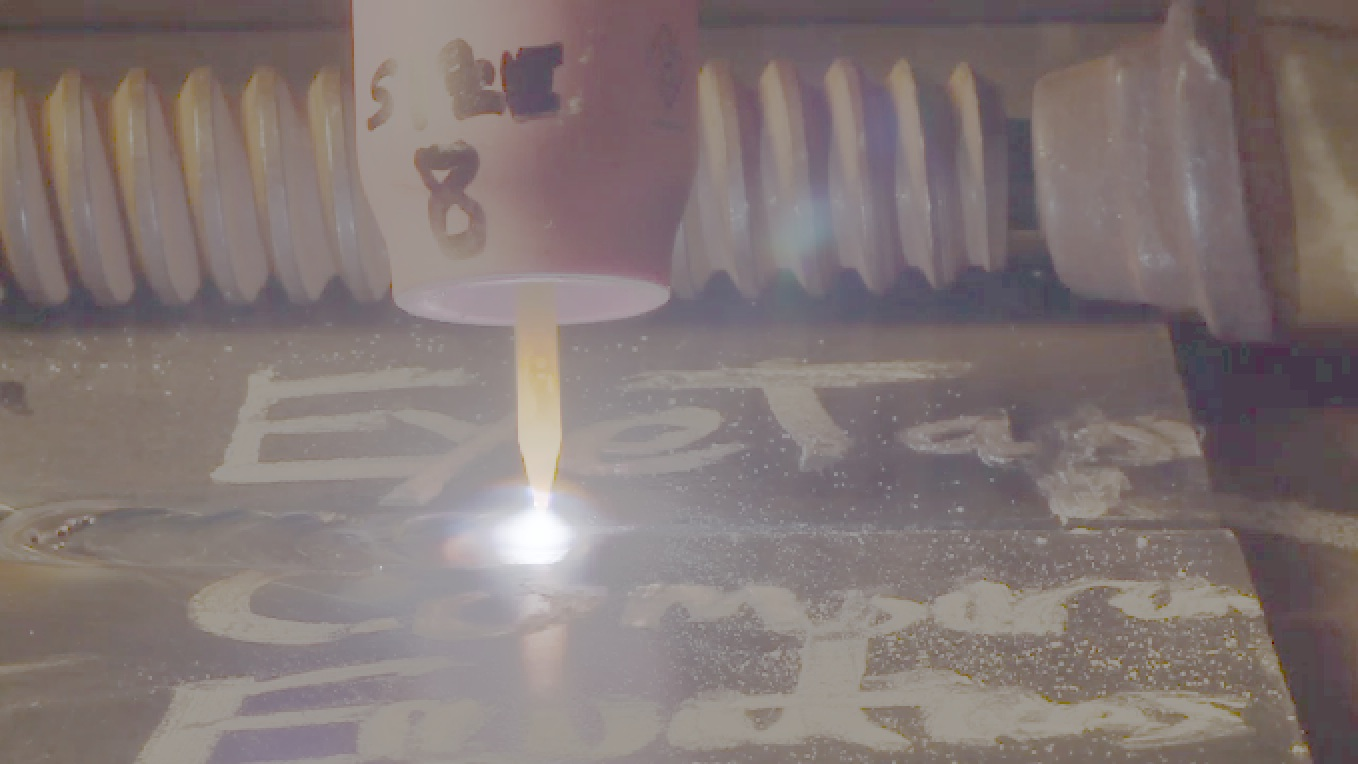
\includegraphics[width=1.4in]{ch2/diagrams/frames/5stops/log_5_stops.jpg}
%\caption{Log Compression}
%\label{fig:log_compress}
%\end{subfigure}
%\begin{subfigure}[b]{1.5in}
%\centering
%\includegraphics[width=1.4in]{ch2/diagrams/frames/5stops/untitled_pregamma_1_mantiuk06_contrast_mapping_0_1_saturation_factor_0_8_detail_factor_1.jpg}
%\caption{Mantiuk, R et al. \cite{mantiuk2006perceptual}}
%\label{fig:mantiuk}
%\end{subfigure}
%\begin{subfigure}[b]{1.5in}
%\centering
%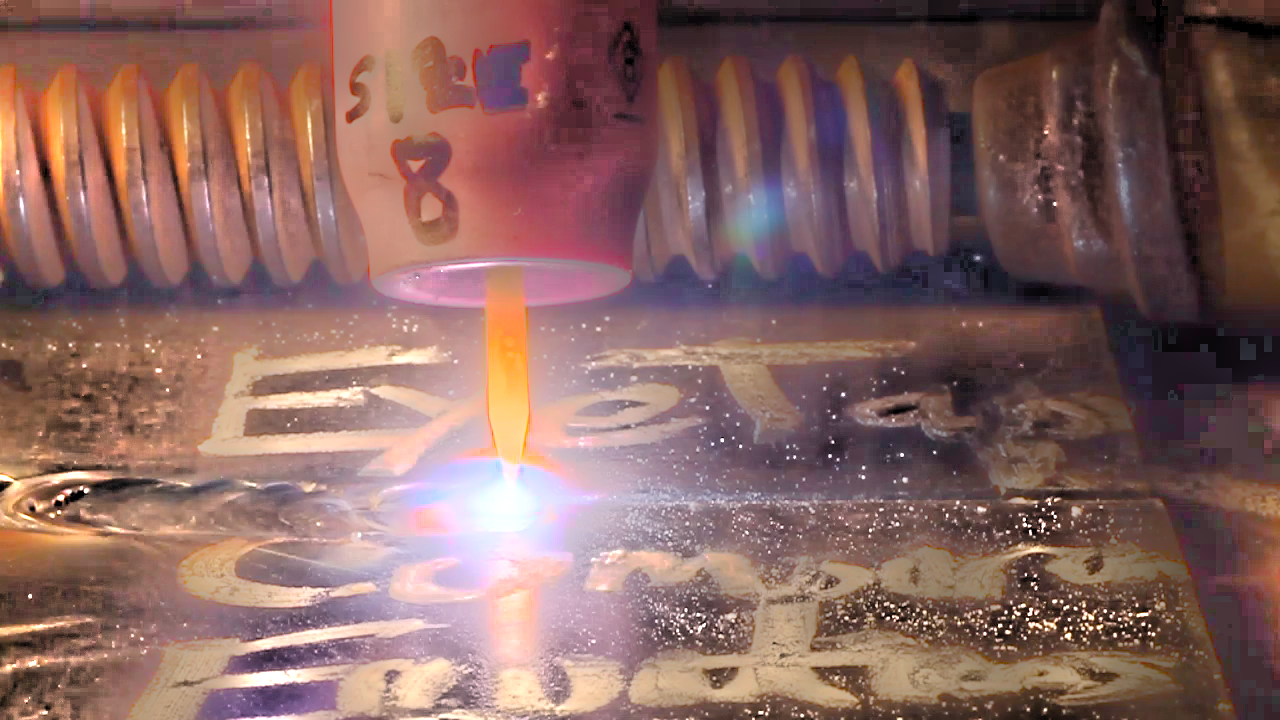
\includegraphics[width=1.4in]{ch2/diagrams/frames/5stops/untitled_pregamma_1_fattal_alpha_0_25_beta_0_57_saturation_0_38_noiseredux_0_fftsolver_1.jpg}
%\caption{Fattal, R. et al. \cite{fattal2002gradient}}
%\label{fig:mouse}
%\end{subfigure}
%\begin{subfigure}[b]{1.5in}
%\centering
%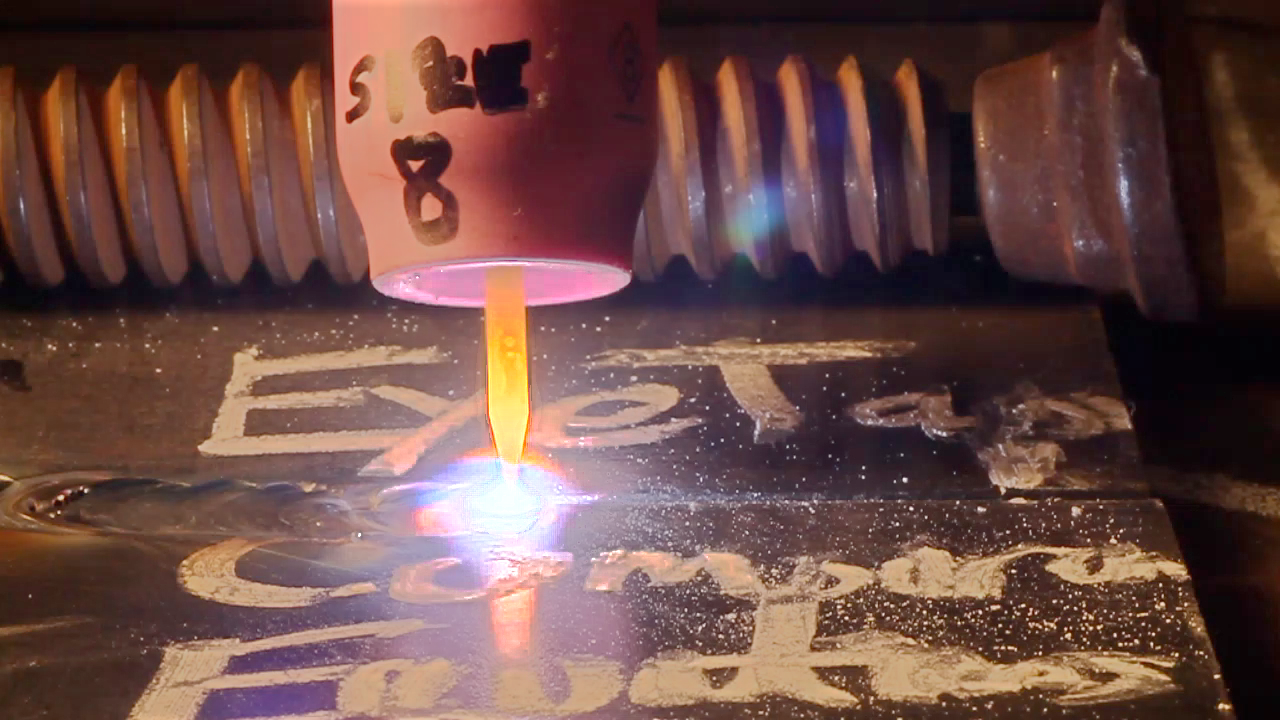
\includegraphics[width=1.4in]{ch2/diagrams/frames/5stops/untitled_pregamma_1_reinhard02_key_0_07_phi_12_2_scales_range_4_lower1_upper90.jpg}
%\caption{Reinhard, E. et al. \cite{reinhard2002photographic}}
%\label{fig:mouse}
%\end{subfigure}        
%
%\begin{subfigure}[b]{6.2in}
%\centering
%  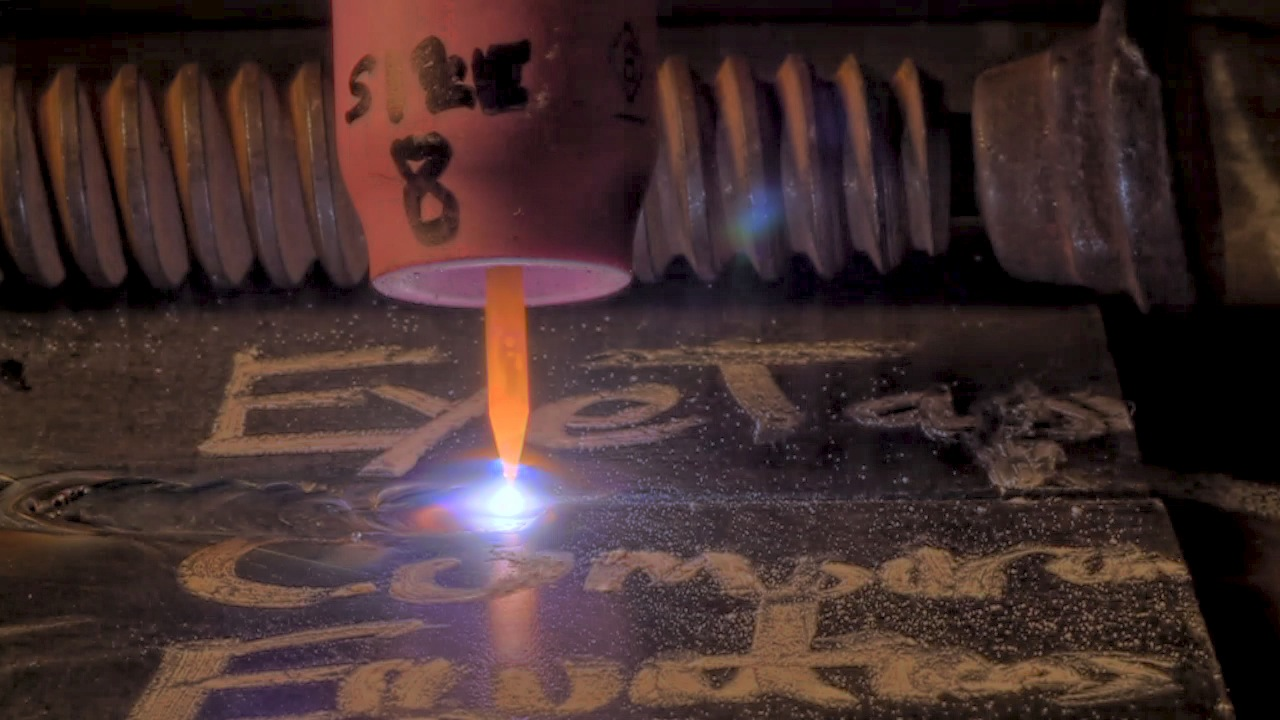
\includegraphics[width=6.0in]{ch2/diagrams/frames/5stops/final_tm_result.jpg}
%  \caption{Our result}
%  \label{fig:mouse}
%\end{subfigure}
%%        ~
%%        \begin{subfigure}[b]{0.22\textwidth}
%%                \centering
%%                \includegraphics[width=4.0cm]{frames/welding_set/dark.jpg}
%%                \caption{whatever}
%%                \label{fig:whatever}
%%        \end{subfigure} 
%\caption{Results for HDR video of extreme dynamic range.
%                 Notice that the tip of the tungsten electrode is only visible
%                 in the darkest exposure, and the background is only visible
%                 in the lightest exposure.
%                 Our result, shown in (b), is the only of the spatiotonemapping
%                 algorithms that can render the very tip of the tungsten
%                 electrode and background both clearly.
%                 (d-f) Tone mapping results from \cite{mantiuk2006perceptual,fattal2002gradient,reinhard2002photographic} using Luminance HDR program.
%                 In extreme cases, the HDR composition method by~\cite{debevec2008recovering} introduced artifacts in the shadow area, and the tone mapping algorithms further amplified these defects in the final images.
%                Our result is not only better than these tone mapping algorithms (and the only one to faithfully show the tip of the tungsten electrode)
%                but it is also capable of running in real-time.}\label{fig:welding_results}
%\end{figure*}
%
%%\begin{figure*}
%%  \center{
%%  \includegraphics[width=4.0cm]{frames/welding_set/dark.jpg}
%%  \includegraphics[width=4.0cm]{frames/welding_set/medium.jpg}
%%  \includegraphics[width=4.0cm]{frames/welding_set/bright.jpg}
%%  \includegraphics[width=4.0cm]{frames/welding_set/stage3.jpg}
%%  \includegraphics[width=4.0cm]{frames/welding_set/untitled_pregamma_1_mantiuk06_contrast_mapping_0_1_saturation_factor_0_8_detail_factor_1.jpg}
%%  \includegraphics[width=4.0cm]{frames/welding_set/untitled_pregamma_1_fattal_alpha_0_21_beta_0_82_saturation_1_noiseredux_0_05_fftsolver_1.jpg}
%%  \includegraphics[width=4.0cm]{frames/welding_set/untitled_pregamma_1_reinhard02_key_0_1_phi_1_scales_range_8_lower1_upper43.jpg}
%%  \includegraphics[width=4.0cm]{frames/welding_set/stage3.jpg}
%%  \caption{The first row shows the differently exposed images of a TIG welding scene.   a) tone mapping by \cite{mantiuk2006perceptual}}
%%  }
%%\end{figure*}
%%
%%\begin{table}[!h]
%%\resizebox{\textwidth}{8mm}{
%%\begin{tabular}{|l|r|r|p{1cm}|}
%
%%\hline
%%Tone Mapping Operator  & Time(ms) & Frames Per Second & Speed-Up using Edge-Preserved \\
%%Tone Mapping Operator  & Time(ms) & FPS & Speed-Up using Edge-Preserved \\
%%\hline
%%Mantiuk, R et al. \cite{mantiuk2006perceptual}                & 1721     & 0.58              & $143.42\times$\\
%%\hline
%%Fattal, R. et al. \cite{fattal2002gradient}                 & 1710     & 0.58              & $142.5\times$\\
%%\hline
%%Reinhard, E. et al. \cite{reinhard2002photographic}               & 154      & 6.49              & $12.83\times$\\
%%\hline
%%Edge-Preserved         & 12       & 83.33             & $1\times$\\
%%\hline
%%
%%\end{tabular}
%%}
%%\caption{This table shows the run-time of different Tone Mapping Operators and shows the speed-up of using our Tone Mapping. Our Tone
%%Mapping algorithm achieves approximately 80 frames-per-second; which is several times faster than other widely used tone mapping operators.}
%%\label{perf_table}
%%\end{table}
%%
%
%In this section, we first discuss a HDR image composition method, which is optimized for GPU or FPGA hardware implementation of electric eyeglasses \cite{mannist,robertson2003estimation,ali2012ICASSP}. Then, we present our approach in creating a real-time HDR video with our pairwise HDR composition and spatial tonal mapping method based on the edge-aware recursive filter (RF)~\cite{GastalOliveira2011DomainTransform}. Together, our proposed algorithm can run in a real-time (30fps or higher on commodity graphics hardware such as NVIDIA 460GTX at 1280x720 resolution) and requires no user intervention in the HDR creation processes.  
%
%%\subsection{Mathematical Notation}
%%We let $f$ as a function represent the \textit{camera response function} (CRF), while $f$ in a scalar context is a \textit{tonal value}, and in a matrix context $f$ is a \textit{tonal image} (e.g. a picture from a camera).  We consider a tonal value $f$ to vary linearly with pixel value but on the unit interval, and given an $n$-bit pixel value $v$ returned from a physical camera, we use $f_i = (v+0.5)/2^n$, where we have $N$ images, $i\in\{1,\ldots,N\},$ and each image has exposure $k_i$. The subscript indicates it is the $i$-th in
%%a \textit{Wyckoff set}\cite{comparam}, i.e.\ a set of images differing
%%only in exposure, and by convention $k_{i}<k_{i+1} \;\forall\; i<N$.
%%We use $f^{-1}$ as the mathematical inverse of $f$ if it has only one
%%argument, and otherwise as a joint estimator\footnote{``Joint
%%  estimator'' is used here in the sense that each photoquantity
%%  estimate depends simultaneously on multiple measurements.} of
%%photoquantity, $\hat{q}$.
%%
%\subsection{Direct Lookup method for combining exposures} \label{comp_2_lut}
%
%For the case of compositing two images with three-color (RGB) channels, one inverse comparametric lookup table (iCLUT) can be derived for each channel for a specific camera sensor. Each entry of an inverse comparametric lookup table results a joint-estimated photometric quantity, $\hat{q}$, from a pair of images captured with different exposures. Each iCLUT is composed of $256\times256$ entries of 8-bit outputs. The iCLUTs need only be calibrated once for every camera.
%
%Each entry of an iCLUT is estimated by the following equation: 
%\begin{equation}\label{joint_est}
%\begin{split}
%  \hat{q}=&f^{-1}_{\Delta EV}(f_1, f_2) \\
%  =&\frac{f^{-1}(f_1) \cdot w_1(f_1)+f^{-1}(f_2) \cdot w_2(f_2) \
%      / 2^{\Delta EV}}{w_1(f_1)+w_2(f_2)}\\
%%\end{cases}
%\end{split}
%\end{equation} 
%where $f_1$ and $f_2$ are the pixel values from a pair images under different exposure settings; $\Delta EV$ is the exposure difference between $f_1$ and $f_2$; $f^{-1}$ is the inverse camera response and $w$ is the certainty function, proposed by Mann\cite{mannist}
%%The camera response function (CRF) f can be determined using the method described by Manders and Mann \cite{mannist}.
%%To construct this look-up-table, we first estimate the response function of the camera along with its certainty function \cite{mannist}.
%%An estimate, $\hat{q}$, of the photoquantity is computed from the pixel (tonal) values $f_1$ and $f_2$. 
%%This can be estimated by the weighted average of the $f_1$ and $f_2$ with respect to their certainty functions $w_i$ and the response function $f$ of the camera.
%
%%\begin{algorithm}
%%\begin{algorithmic}
%%\Procedure{RF}{$I$}
%%	\State $\left[\frac{dH}{dx}, \frac{dH}{dy}\right] \gets Calculate\_Gradient(I)$
%%	\State $Transpose\_Image(I)$ \Comment{Rows become columns}
%%	\State $RF\_Y\left(I, \frac{dH}{dx}\right)$            \Comment{To process the rows}
%%	\State $Transpose\_Image(I)$ \Comment{Revert to original image}
%%	\State $RF\_Y\left(I, \frac{dH}{dy}\right)$            \Comment{To process the columns}
%%\EndProcedure
%%\end{algorithmic}
%%\caption{Computation of a single entry in an iCLUT}
%%\label{RF_pseudo}
%%\end{algorithm}
%
%
%%
%%However, in extreme cases the images are several stops apart. It is important that the certainty function provides additional weighting to the brighter image to reduce the gain $2^{\Delta EV}$ to the shadow area in the last step.
%
%\subsection{HDR Composition for 3 or more Images} \label{comp3_set} 
%For the case of constructing HDR images from N images (for N $\ge$ 3), we compute $log(N)$ levels of pairwise estimate of the photometric quantities, $\hat{q}_{h,i}$, read as the $ith$ pairwise estimate of photometric quantity at level $h$. At the top level, we compute $\hat{q}_{log(N),i}$ using iCLUT generated by Eq.~\ref{joint_est}. For each of proceeding level, its corresponding set of $\hat{q}_{h,i}$ is estimated by: 
%\begin{equation}
%\hat{q}_{h,i}=\frac{\hat{q}_{h-1,j}\hat{w}_{h-1,j}+\hat{q}_{h-1,j+1}\hat{w}_{h-1,j+1}/ 2^{\Delta EV}}{\hat{w}_{h-1,j}+\hat{w}_{h-1,j+1}}
%\end{equation}
%where
%\begin{equation}
%\hat{w}_{h,i}=\max(\hat{w}_{h-1,j},\hat{w}_{h-1,j+1})
%\end{equation}
%
%
%%\begin{equation}
%%\hat{q_i}=f^{-1}_{\Delta EV}(f_i, f_{i+1}), i \in \{1,..,N\}
%%\end{equation}
%
%%Then, we combine the individual photoquantity $\hat{q_i}$ with the
%%certainty values $\hat{w_i}$ computed from last step with:
%%\begin{equation}
%%\hat{q}=g(\hat{q_i}, \hat{q}_{i+1}, ... , \hat{q}_{N-1}, \hat{w_i}, \hat{w_{i+1}},...,\hat{w_{N-1}})
%%\end{equation}
%%to create our final estimate of $\hat{q}$.  For the case of 3 images,
%%the function $g$ can be implemented as a simple weighted average of
%%the $q_1$ and $q_2$ with respect to the certainty values $\hat{w_1}$ and
%%$\hat{w_2}$:
%%\vspace{-.1in}
%%\begin{equation}
%%\begin{split}
%%  \hat{q} = g(\hat{q}_1, \hat{q}_2, \hat{w}_1, \hat{w}_2) = \frac{\hat{q}_1 \cdot
%%    \hat{w}_1 + \hat{q}_2 \cdot \hat{w}_2 / 2^{\Delta EV}}{\hat{w}_1+\hat{w}_2}
%%\end{split}
%%\end{equation}
%
%
%%One advantage of our proposed algorithm is that we have reduced the problem
%%into sub-steps that we can easily optimize for specific algorithm, and
%%can provide a significant speedup in those cases. 
%%\begin{figure}
%%  \includegraphics[width=3.5in]{siggraph2010_ch2/diagrams/4_composite_2.pdf}
%%  \caption{Composition of HDR images using our pairwise approach for
%%    combining four LDR images, $f_1$, $f_2$, $f_3$, and $f_4$. The final
%%    estimate of the photoquantity $\hat{q}$ then undergoes our hardware-accelerated tonemapping algorithm.  }
%%  \label{composite3}
%%\end{figure}
%
%By capturing 4 images with $\Delta EV=4$, the dynamic range of the HDR image spans a total of 20 stops $(2^{20}=1,048,576)$ approximately a million to one contrast ratio. To display such wide range on the LDR display, the photoquantity $\hat{q}$ will be compressed with a multi-scale spatial-tonal mapping algorithm.
%%
%% history here
%%
%
%\subsection{Global Histogram Equalization}
%With the power/logarithmic compression, the $\hat{q_c}$ often cluster in a narrow range of values and thus under-utilizing the displayable range (see Fig.~\ref{fig:welding_results} (c)). To re-distribute $\hat{q_c}$ to have a uniform occupancy across the possible displayable range, we adopted the histogram equalization (HE) as the technique to recover the global contrast from the HDR image. Since $\hat{q_c}\epsilon[0,max(\hat{q_c}))$, normalization is required to bound $\hat{q_c}$ in a known range. To perform HE, we need to construct a histogram of the image as well as the cumulative sum of the histogram:
%%h($\cdot$) as equalization operator and $\hat{q_h}$ as equalized estimator,
%\begin{equation} \label{histogram_regular}
% \hat{q_h}=HE(\hat{q_c})=\frac{cs(\hat{q_c})-cs_{min}}{M-cs_{min}}max(\hat{q_c})\\
%\end{equation}
%where $M$ denotes the number of pixels in the image and $cs(v)$ results the cumulative sum of $v$ from its histogram. It is known that Equation~\ref{histogram_regular} may over-stretch $\hat{q_c}$ at spikes in a histogram (e.g. $h_k \gg h_{k+1}$ and $h_k \gg h_{k-1}$). This may yield undesirable result since $\hat{q_c}$ is concentrated in a narrow range of values. The outcome of the equalized image then compresses the contrast of brightest and darkest light values and results a LDR like image. To resolve this behaviour, we apply histogram modification proposed by~\cite{lee2012power}:
%\begin{equation} \label{histogram_regular}
% m_k=\frac{\log(h_kh_{max}10^{-\mu}+1)}{\log(h_{max}^{2}10^{-\mu}+1)}\\ 
%\end{equation}
%\begin{equation}
% cs(k)=\displaystyle\sum\limits_{i=0}^{k-1}m_k
%\end{equation}
%where $m_k$ is the modified value of the original value of histogram at bin k, $h_k$. The choice of $\mu$ moderates the change to the histogram. For large $\mu$, the histogram becomes nearly uniform, whereas, for small $\mu$ $\ll$ 1, the histogram remains approximately unchanged. We have chosen $\mu$ = 5 which results a much more uniformly distributed histogram. Consequently, it reduces the over-stretching effect of equalization.
%
%\section{Multi-scale Spatial Tonal Mapping}
%%halo free, much less artifact than the other two (compare with fatal,etc...)
%%With a global tonal mapping operator, the HDR result obtained from the previous section appears relatively low in contrast and saturation when dealing with extreme dynamic range scene (See Figure~\ref{lamp_set}). To improve the visual appearance of the images on LDR display, we can compress the HDR image based on the not only tonal information, but also spatial information such as gradient and edges. Although a number of tone mapping algorithms had been proposed, very few tone mapping algorithm been designed for the real-time video usage. Particularly, the tone mapping which shows high quality results often involves non-linear optimizers which has a high complexity and difficult to be parallelized due to its non-deterministic runtime. On the other hands, results from \cite{reinhard2002photographic}, which has low computation requirements and easy to parallelized, produce poor looking results with halo artifacts, low contrast, and non-natural looking results. Moreover, some of the tone mapping operators are only designed for images and produce temporal artifacts such as flickering and color shifting throughout the process.
%%Recently, a computationally efficient edge-preserving filter \cite{chen2007real, GastalOliveira2011DomainTransform} has shown promising results in performing tone mapping on HDR images. %The recursive filter (RF) ~\cite{GastalOliveira2011DomainTransform} is shown to be particularly well-suited for decomposing the image in real-time on graphics hardware.
%Our approach for real-time tone mapping and composition, which is based on \cite{GastalOliveira2011DomainTransform} and \cite{farbman2008edge}, provides the natural looking and stable results among a large variety set of conditions (see Fig.~\ref{fig:welding_results} for comparison).
%%The contribution of our work is the design of a complete HDR algorithm that can run on graphics hardware or FPGAs in the future.
%%list a few tone mapping algorithms here%
%%see figure for the L value.
%%see the compressed value
%%decomposition
%%detail layers
%%controls
%%
%%see the final value
%%\subsection{Global Dynamic Range Compressor}
%To compress the high dynamic range images we first estimate the log luminance, $L_c$, of the image based on the final estimate of photoquantities on the RGB channels, $\hat{q}_r$, $\hat{q}_g$, $\hat{q}_b$, from section 2.2.
%\begin{equation}
%L_c = log(0.2989*\hat{q_r} + 0.5870*\hat{q_g} + 0.1140*\hat{q_b} + 1).
%\end{equation}
%Then, the dynamic range of the luminance channel is compressed using a logarithmic compressor with a simple offset to avoid negatives values.
%\begin{equation}
%L_c = log(L+1).
%\end{equation}
%Alternatively, we found that we can achieve a more natural looking, but less contrast result with the following compressor.
%\begin{equation}\label{lum_equation_2}
%L_c = L^{l/\gamma}
%\end{equation} where $\gamma \ge 1$ and $c$>0.
%
%Then, the $L_c$ is normalized and compressed to the range $[0,1]$. Then, we can adjust the range, which has later effect on the detail extraction, with the $s$ and $d$ parameters (typically set to $s=8.0$, $d=5$).
%\begin{equation}\label{lum_equation_3}
%L = s*L_c+d
%\end{equation}
%In our setup, we have applied a moving average filter on $max_L$ and $min_L$ to avoid flickering due to any sudden luminance changes in the scene.
%
%\subsection{Local Contrast Enhancement}
%The global tone mapping, such as logarithmic compression, from the last step provides us a base image which is often lacking contrast. We can enhance the local contrast (spatial-tonal mapping) with the multi-scale edge-preserving decomposition method. This method is found to be effective for compressing HDR images at extreme cases (see the clear rendition of the tip of the tungsten electrode with our proposed method in Fig. 1b).
%To extract details from the image and enhance their local contrast, we first create the multi-scale edge-preserved smoothed image $J_i$ where i $\in\{1,..,M\}$ using the recursive filter (RF) discussed in \cite{GastalOliveira2011DomainTransform}.
%\begin{equation}\label{lum_equation_4}
%J_i = RC (L, \sigma_s, \sigma_r, k)
%\end{equation}
%where $\sigma_s$ and $\sigma_r$ are the filter spatial and range standard deviation, and k is the number of iterations the filter smooths the image. In particular, we use $\sigma_s$ = 20, $\sigma_r$ = 0.0825 for $J_1$; $\sigma_s$ = 50, $\sigma_r$ = 0.165 for $J_2$; $\sigma_s$ = 100, $\sigma_r$ = 0.335 for $J_3$ and $k=1$. We obtain the detail layers $D_i$ by finding the difference between $J_{i-1}$ and $J_i$, with $J_0=L$, where each succession of the detail layer contains coarser details than the previous layer. The detail layers are weighted and summed to reduce to a single contrast mask $L_f$ as the following:
%\begin{equation}
%L_f = 0.9*J_M + \sum_{i=0}^{M-1}{a_i D_i}
%\end{equation} where $a_i$ is the desired weight for each layer. In our setup, we have used $a_0=0.4$, $a_1=0.3$, $a_2=0.3$ which emphasize the texture from the layer containing the finest details. By our observation, this setting allows greater local contrast of tonal values at the extreme bright and dark areas of the scene. To obtain a displayable output image, we compress the photoquantity $\hat{q}$ using the contrast mask in eq.\ref{lum_equation_4} and quantize the results to the standard 24 bit RGB pixel values:
%\begin{equation}
%\begin{split}
%f &= round(255.0*(\hat{q}/10^{L})^{\gamma} \cdot L_f), \\
%\end{split}
%\end{equation}
%
%
%Table~\ref{table:layers}.
%\vspace{-0.5cm}
%\begin{table}[!h]
%\center
%\caption{The parameters for the 3 detail layers used in our system.}\label{table:layers}
%\begin{tabular}{|c|c|c|c|}
%\hline
% & $J_1$ & $J_2$ & $J_3$ \\
%\hline
%$\sigma_s$ & 20.0 & 50.0 & 100.0 \\
%\hline
%$\sigma_r$ & 0.0825 & 0.165 & 0.335 \\
%\hline
%\end{tabular}
%\end{table}
%From our experiment, this filter is more computationally efficient than bilateral filter n large kernel size. This is a critical requirement to our HDR compression algorithm as the runtime remains constant regardless of the parameters settings. Furthermore, does not introduce temporal artifacts (such as flickering) and the results is consistent (e.g., the histogram equalization approach often result in inconsistent results under difficult lighting condition). This is critical in HDR video because any incoherence between the adjacent frames can be distracting to the audience.
%Once we have obtained the smoothed edge-preserving images, the detail layers from is extracted by subtracting the adjacent images from the stack.
%\begin{equation}
%D_i = J_i - J_{i+1}
%\end{equation} where $J_0=L$, and i $\in \{0,..,K-1\}$.
%Then, we can compose our results by first normalizing the $J_N$ channel as our base image with the following linear mapping:
%\begin{equation}
%B = \frac{J_K - min_J}{max_J - min_J}
%\end{equation}
%where $[min_J, max_J]$ is the desired range we would like for the LDR image.
%where $max_J$ and $min_J$ are the desire range we would like to mapped to our LDR.
%where the parameter $\gamma$ controls the saturation in the final image, and we typically set them between $0.5$ to $0.7$.
%
%
%Overall, there are two main advantages of using the edge-preserving filter proposed by \cite{GastalOliveira2011DomainTransform}. First, the parameters $\sigma_s$ and $\sigma_r$ empower users to refine their emphasis of detail enhancements. Second, the fine tuning of $\sigma$ parameters helps minimizing the halo artifacts when comparing to traditional image decomposition based on laplacian pyramid. Qualitatively, the output of our HDR rendition is comparable to many other approaches as shown in Fig~\ref{fig:welding_results}.
%%It is worth noting that this tone mapping algorithm is size dependent. For higher resolution videos, it may be necessary to use additional layers (e.g., 4 layers instead of 3 in this case). Fortunately, the algorithm proposed is independent of other parameter settings such as brightness, contrast, and detail manipulation, since the size of the video is constant. These properties are critical to the design of a HDR system that would be used in day-to-day life. Furthermore, our proposes solution shall be scalable to higher resolution as more capable hardware becomes available in the future.
%\section{Performance}
%%The algorithms described in previous sections were specifically chosen and designed to be parallelized on GPUs and simplified for direct hardware implementation on FPGAs.
%%To show the feasibility of our approach, the Direct LUT method described in Section~\ref{comp_2_lut} were implemented with the 3 alternating frames on FPGAs.
%\subsection{GPU}
%\begin{table}[!h]
%\center
%\begin{tabular}{|l|r|r|}
%\hline
%%Tone Mapping Operator  & Time(ms) & Frames Per Second & Speed-up \\
%\bf{Tone Mapping Operator} & \bf{FPS} & \bf{Speed-up}\\
%\hline
%Mantiuk, R. et al. \cite{mantiuk2006perceptual}     & 0.58              & $143.42\times$\\
%\hline
%Fattal, R. et al. \cite{fattal2002gradient}        & 0.58              & $142.5\times$\\
%\hline
%Reinhard, E. et al. \cite{reinhard2002photographic}     & 6.49              & $12.83\times$\\
%\hline
%Implemented Edge-Preserving Method          & 83.33             & $1\times$\\
%\hline
%\end{tabular}
%\caption{This table shows the run-time of different Tone Mapping Operators and the speed-up of using our implemented method. Our implementation 
%achieves approximately 80 frames-per-second; which is several times faster than other tone mapping operators.}
%\label{perf_table}
%\end{table}
%
%Computation using GPU maximizes acceleration on algorithms that run on a large matrix with independent element operations. Our proposed HDR algorithm heavily relies on per pixel operation without much cross dependencies with neighbour pixels. In the following discussion, we layout the runtime cost of each operation in milliseconds, benchmarked on a NVIDIA 460GTX, over 150 videos at the resolution of 1280x720. The operations of pixel-to-photoquantity conversion and the compression by logarithm consume on average of $1.5ms$. Normalization on images are done using efficient min/max finder from NVIDIA's CUBLAS library, which costs around $0.8ms$ per call. The spatial tone mapping is the least parallelizable part of the process, which consumes up to $12ms$. The edge-preserving filtering for three layers executed in parallel takes up $11ms$ of runtime, becomes the main contributor to the overall latency in our proposed HDR pipeline. This is due under utilization of available thread pool of the GPU architecture. Per iteration the RF only requires as many threads as the size of one dimension of the image multiplied by the number of color channels. In our proposed implementation, we launch the filter on a monotone channel, $L$, to reduce the total amount of computation required. Other optimization technique such as matrix transpose is applied to ensure coalesced memory access patterns. The remainder of $1ms$ runtime is contributed by the contrast enhancement stage after obtaining the layers using RF. Overall, the HDR composition and tonal range compression algorithm cost $17ms$ (~60fps) on average, and that is suitable for real-time system. 
%%The general rule in GPU computing is to avoid excessive memory transfer between the machine and graphics card. In our application, since every step can be computed using GPU, the memory transfer is only required upon receiving a new frame. Since the transfer overhead with latency is as low as 1$ms$ per frame per direction (e.g., host to device or device to host), it is relatively insignificant comparing to the latency due to the construction of HDR image. Global memory access on GPU is usually expensive in comparison to shared memory and thread cache. Frequent access to read/write global memories as intermediate update could cause high latency and drop performance of the construction. Another expensive operation is due to thread synchronization after each kernel call. Therefore, 
%
%%\begin{table}[!h]
%%\center
%%\caption{Average latency per stage of HDR construction for a $1280\times720$ image on a NVIDIA Tesla C2050 with 3 detail layers.}
%%\begin{tabular}{|l|c|}
%%\hline
%%Operation & Time (ms) \\
%%\hline
%%Light space conversion & 1.5 \\
%%\hline
%%Local Contrast Enhancement with RF & 24.0 \\
%%\hline
%%\end{tabular}
%%\end{table}
%
%
%%\subsection{FPGA}
%%
%%The algorithm which uses direct look up table is implemented on a Spartan-6 LX45 FPGA device for its low power consumption and portability. %(See Fig~\ref{fig:FPGAHDRchitecture}). 
%%The supply power measured for the system is 1.448W, thus it allows the application to run for around $20$ hours on a typical rechargeable battery with capacity of $5800$mAh.
%%The board contains High Definition Multimedia Interface (HDMI) input ports used to receive video in $720\times480$ at 60 frames per second, and output HDMI ports used to transmit HDR video frames. 
%%Two differently exposed video frames of the same subject matter are supplied via the HDMI input in rapid succession, in an alternating order.
%%The frames are stored into memory and read out concurrently for composition.
%%The 128MB of DDR SDRM (Micron MT47H64M16-25E, 16-bit data width) on the board is configured to run at 625MHz data rate to store video frames.
%%The board also contains 2.1Mbits (116x18432bits) Block RAM (BRAM) in total, which are used for line buffers and to store pre-computed LUT results.
%%
%%The post processing starts by compressing the produced HDR images with a square root.
%%Then it converts the color space from RGB to YCrCb, in order to save the resources that needed for implementation. Converted luma channel is convolved with multi-stage a 5-by-5 Gaussian Kernel for extracting two layers of edges from the original HDR image.
%%The edges are then scaled and added back to the original image for bringing back the detailed textures.
%%
%%The 4-up display mode was created to provide a real-time visualization of multiple exposures,  
%%  enabling the user to simply point a camera and see the frames that comprise the HDR composition. 
%%This allows for easier testing and calibration of the input frames for HDR video processing %(See Fig~\ref{diagram_4up}).
%%The maximum latency of the implemented logic is 223ns, whereas the DDR2 memory access used up 80 percent of the processing time.
%
%%\begin{figure}
%%\center
%% \includegraphics[width=7.5cm]{fpga_images/acmmm12_fpga.pdf}
%% \caption{FPGA-based HDR architecture for the 4-up display capabilities.}
%% \label{fig:FPGAHDRchitecture}
%%\end{figure}
%
%%\subsubsection{Real-time HDR Streaming Using 2 frames}
%%Real-time HDR composition of 2 differently exposed frames was implemented using direct look-up tables (LUTs).
%%For combining two images~\cite{ccece2012hdrEyetap}, pre-computed 8-bit values are stored into Block RAMs (BRAM).
%%In order to implement one LUT, it requires 65556-entries (256 x 256) times 8 bits per entry, which is equivalent of 524kbits. 
%%This requires 1.5Mbit (524kbits x 3 channels of RGB) to cover the two images with 8-bit RGB color space.
%%Since the Spartain-6 FPGA contains 2.1Mbits of BRAM, a more efficient memory utilization method is required to enable HDR involving more than two frames. 
%
%%\subsubsection{4-up HDR display, enabled by FPGA}
%%Push buttons and switches connected to the FPGA are configured such as to enable switching the order of dark, medium, bright frames, and turning on/off 4-up mode. 
%%To be included as a hand-held screen for the final prototype for portable real-time HDR device, this 4-up screen enables users to calibrate exposures quickly and accurately on the go.  
%
%%In the process of implementing the 4-up display, a constraint was put on the design to ensure that no change was required to the original data path. 
%%This requirement was crucial to the overall modular design of our FPGA HDR architecture. 
%%This only adds two modifications to the original data path, both of which are controlled via push-button switches. The switches allow for easy change to the original data path without the 4-up - useful for when the full-screen or eyeglass-mounted display or EyeTap resolution is desired for just the combined HDR video.
%
%%diagrams for the flow
%%fixed aperture (DOF) 
%%low ISO (noise)
%%only alter the shutter speed
%
%\section{Results and Applications}
%
%\begin{figure}
%\center
% 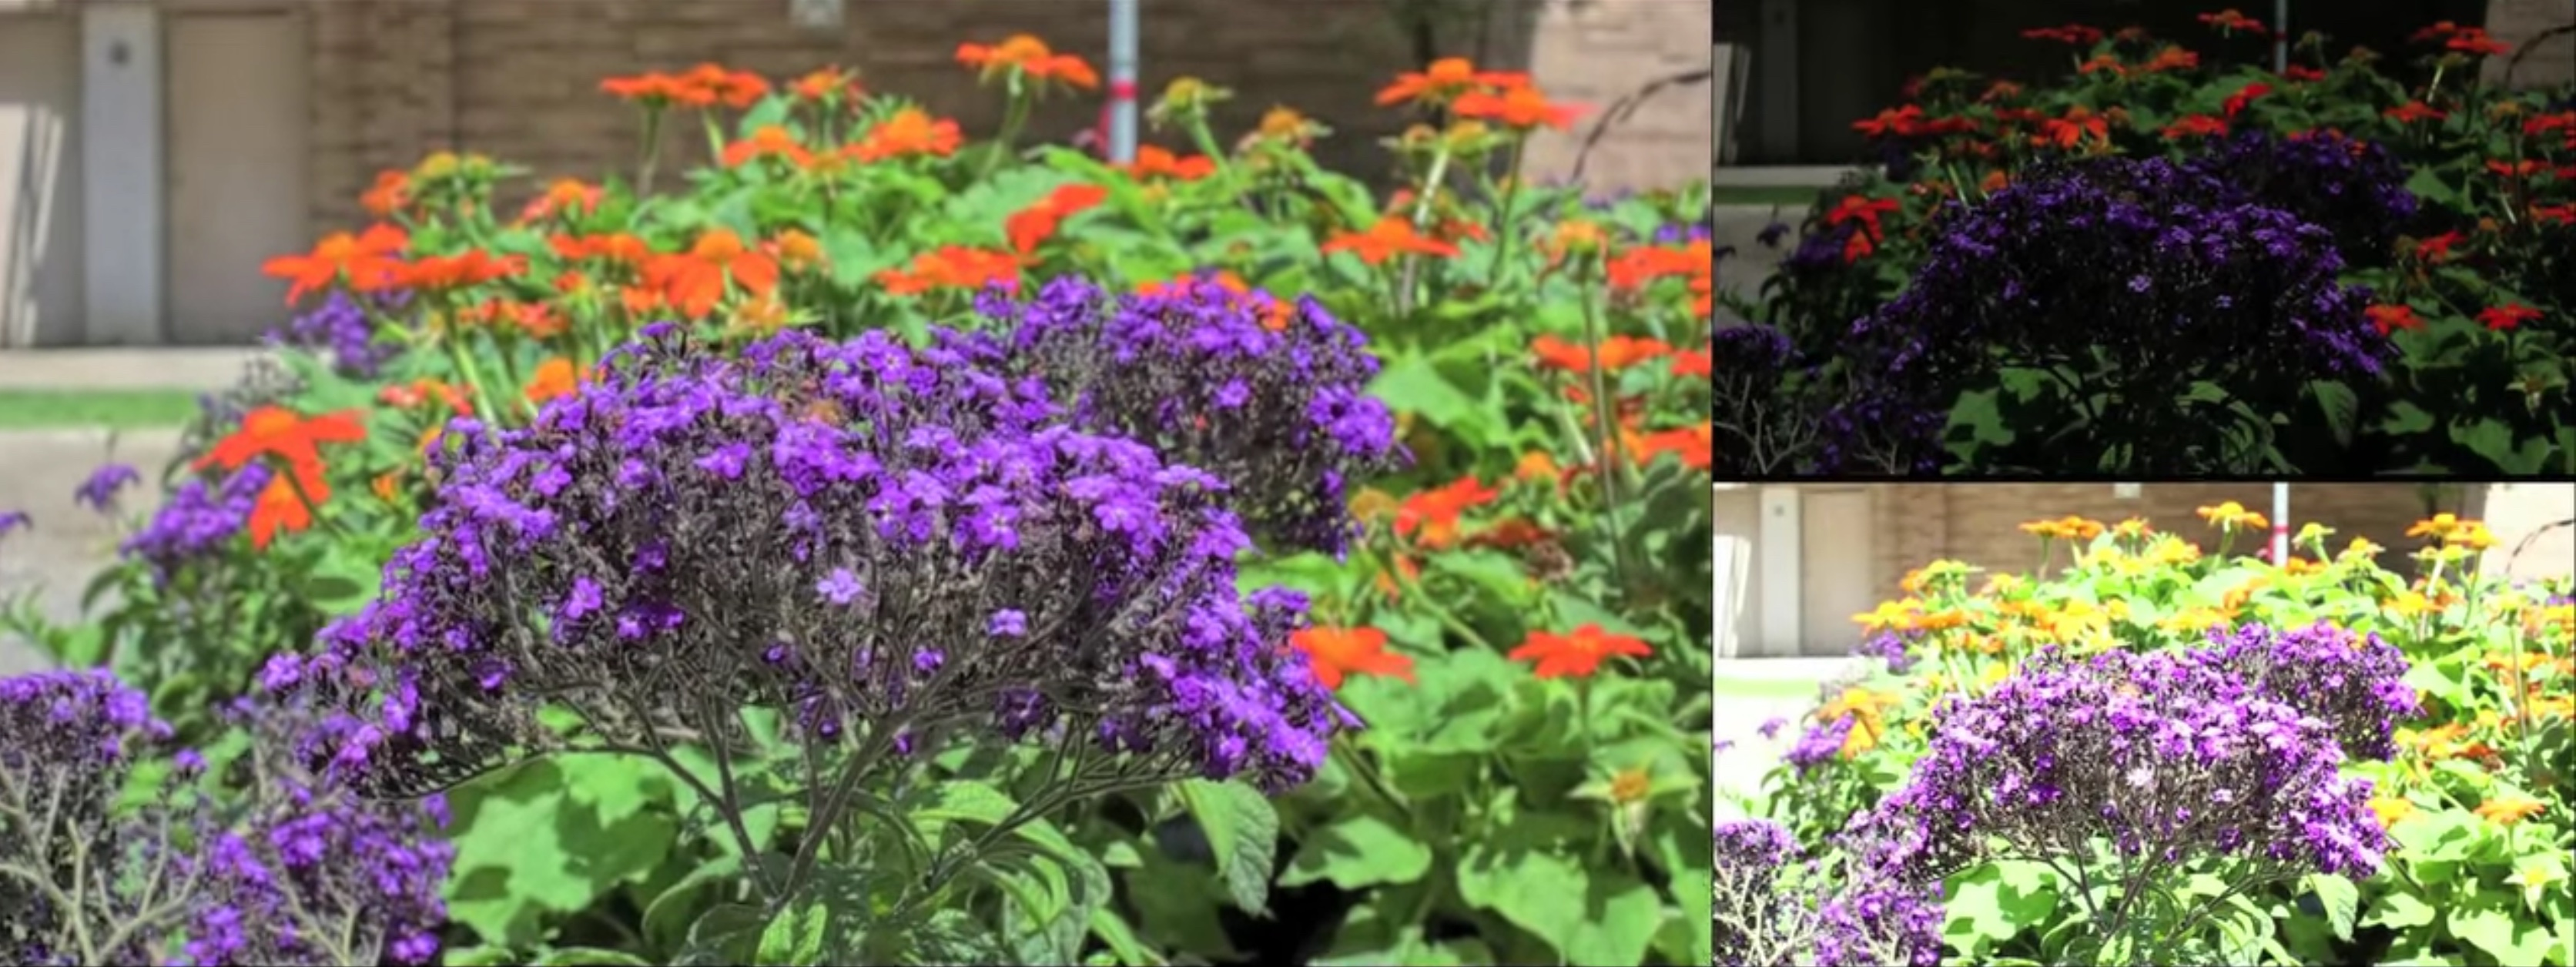
\includegraphics[width=5in]{ch2/diagrams/everyday1.png}
% \caption{}
% \label{fig:extremeeveryday1}
%\end{figure}
%
%\begin{figure}
%\center
% 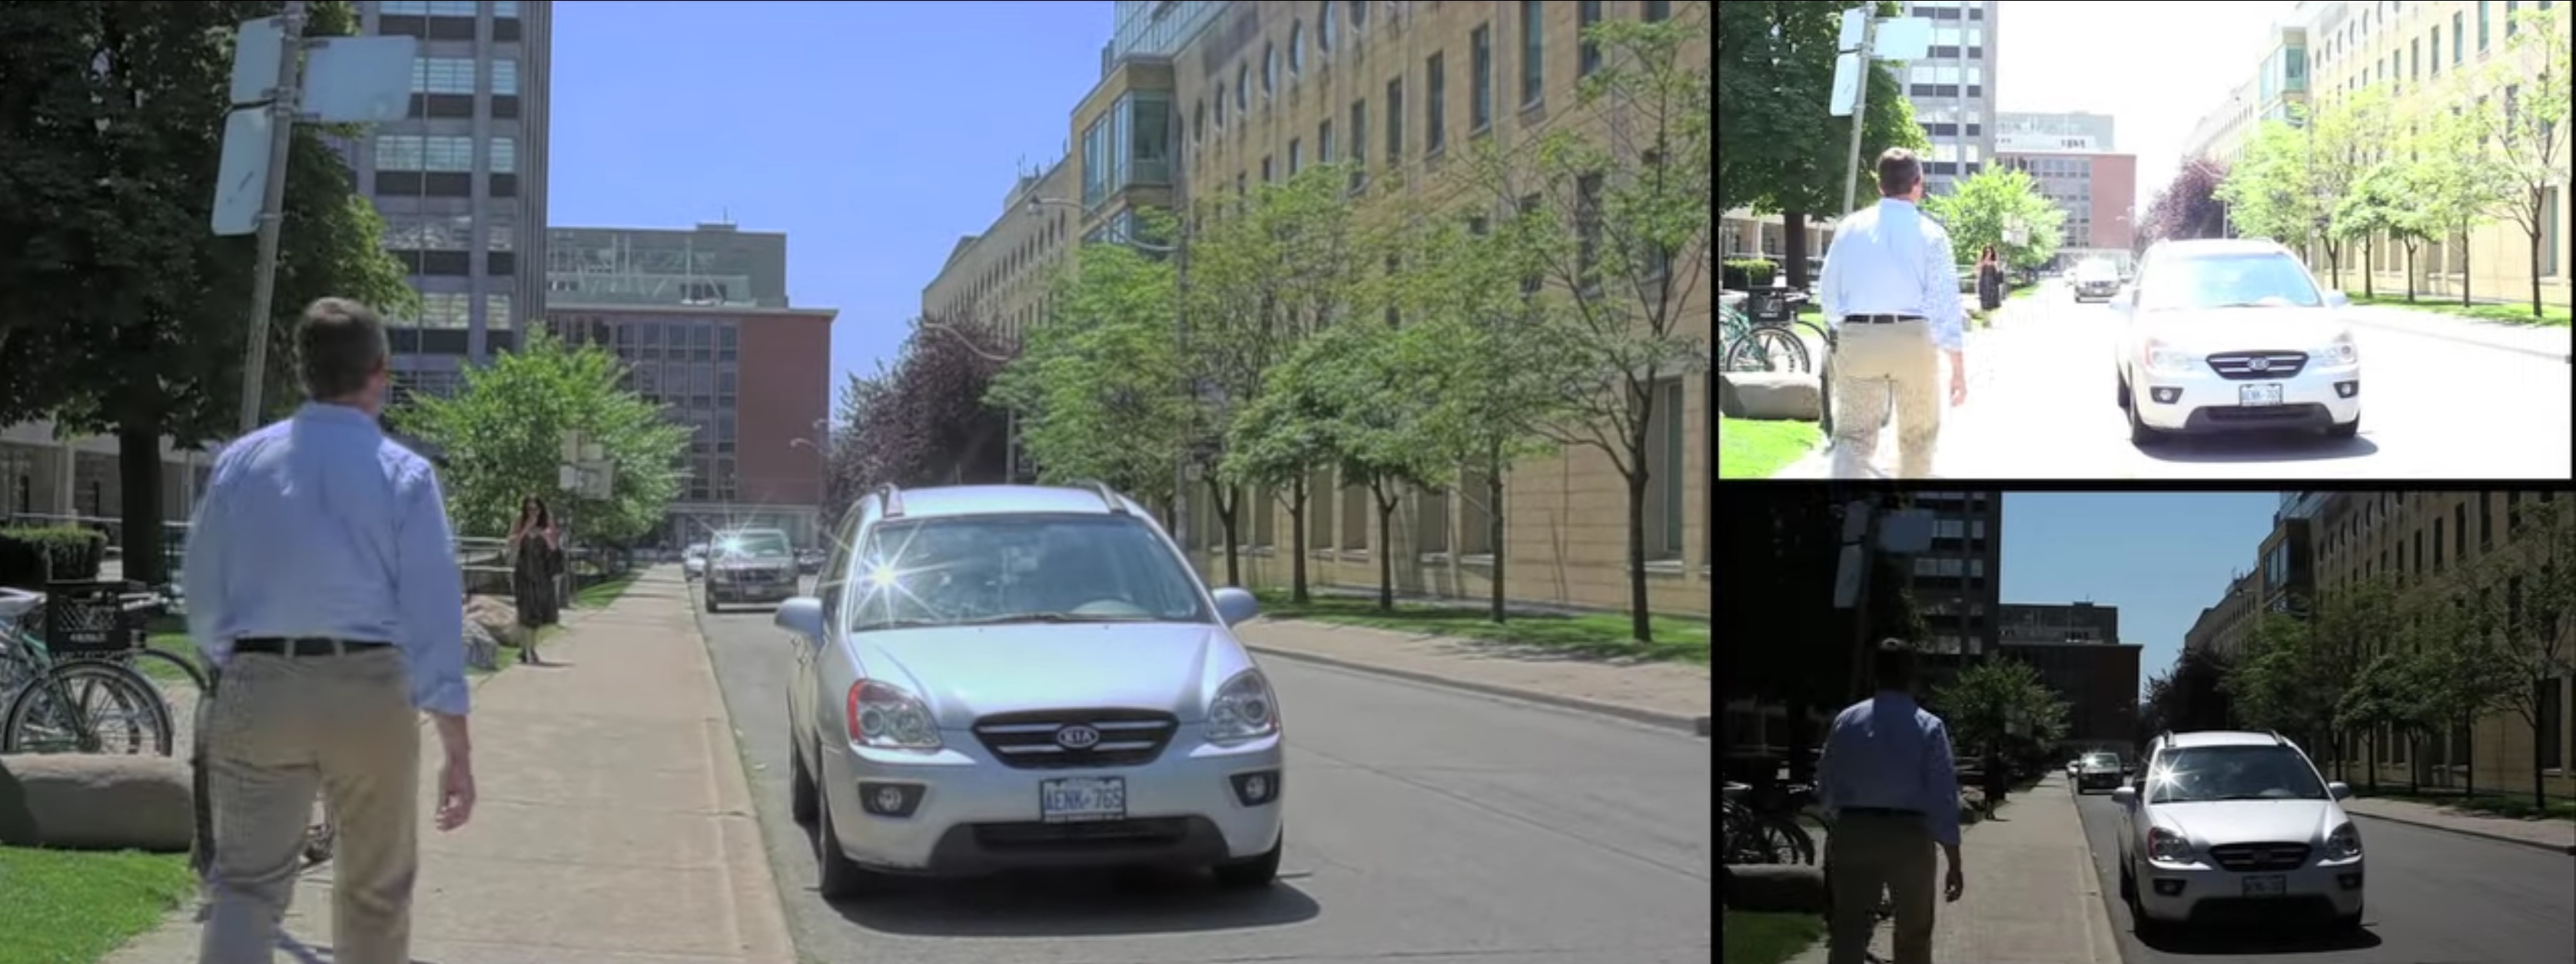
\includegraphics[width=5in]{ch2/diagrams/everyday2.png}
% \caption{}
% \label{fig:extremeeveryday2}
%\end{figure}
%
%\begin{figure}
%\center
% 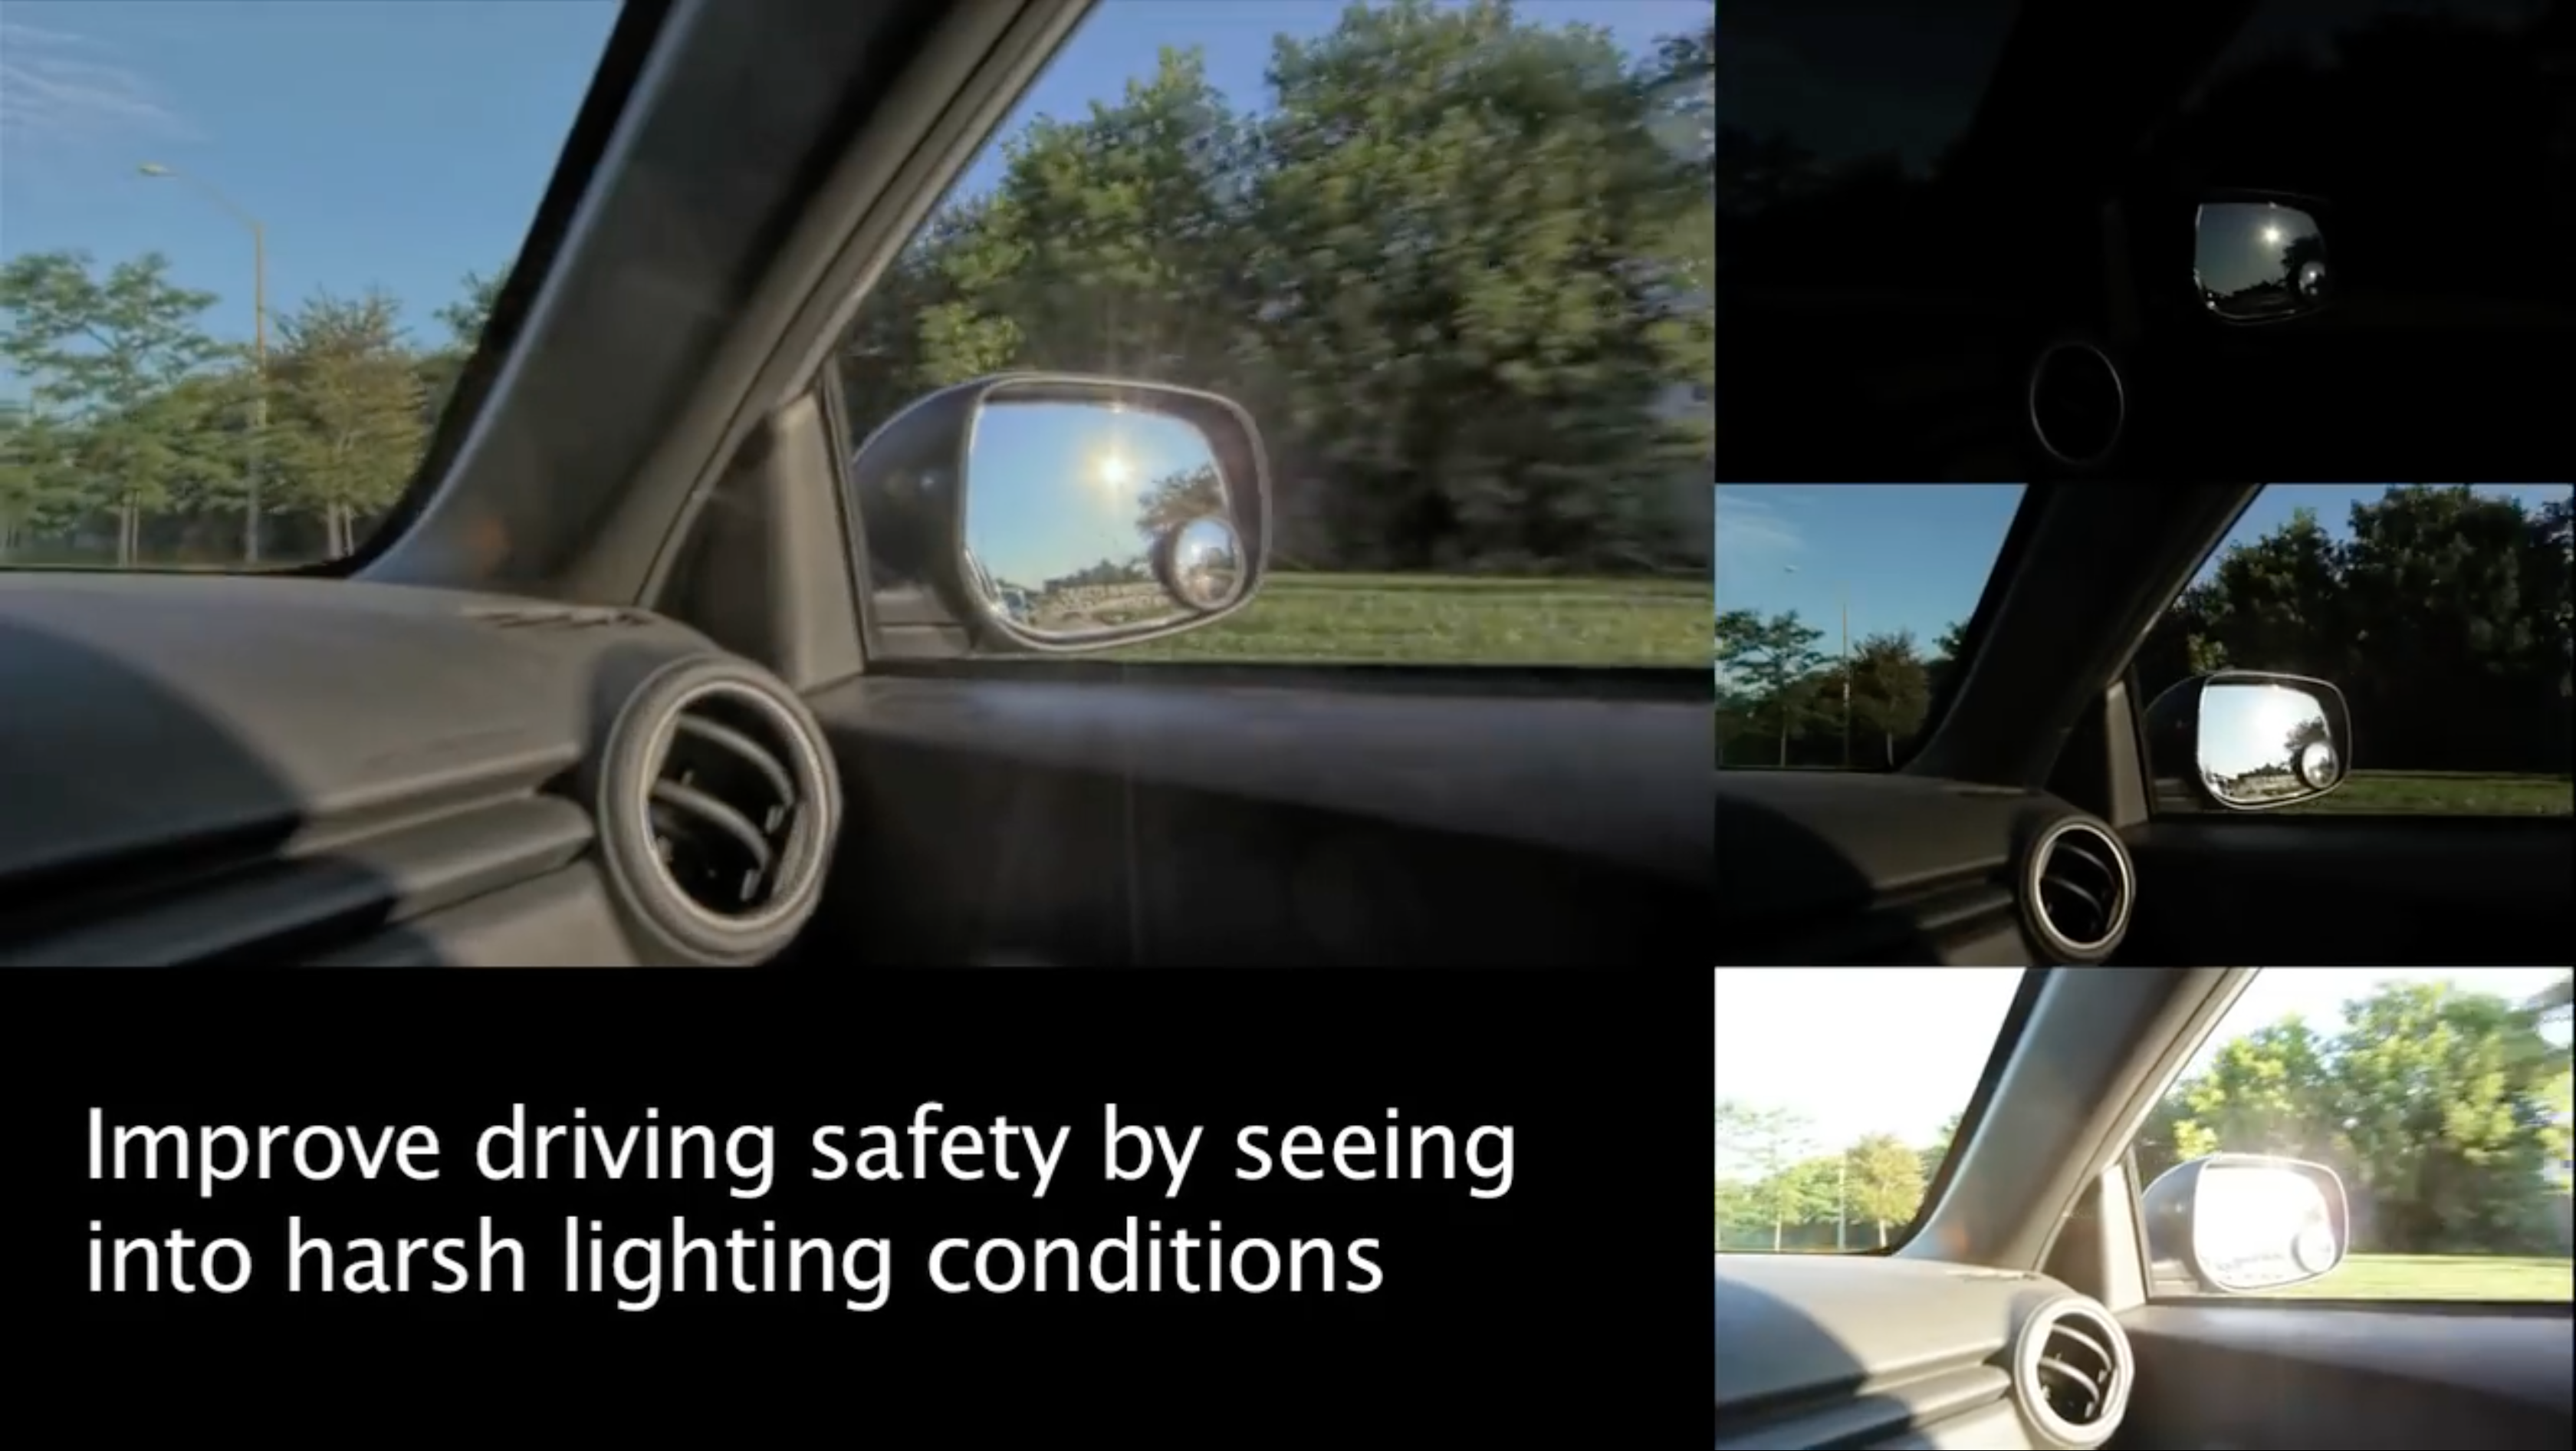
\includegraphics[width=5in]{ch2/diagrams/everyday3.png}
% \caption{}
% \label{fig:extremeeveryday3}
%\end{figure}
%
%\begin{figure}
%\center
% 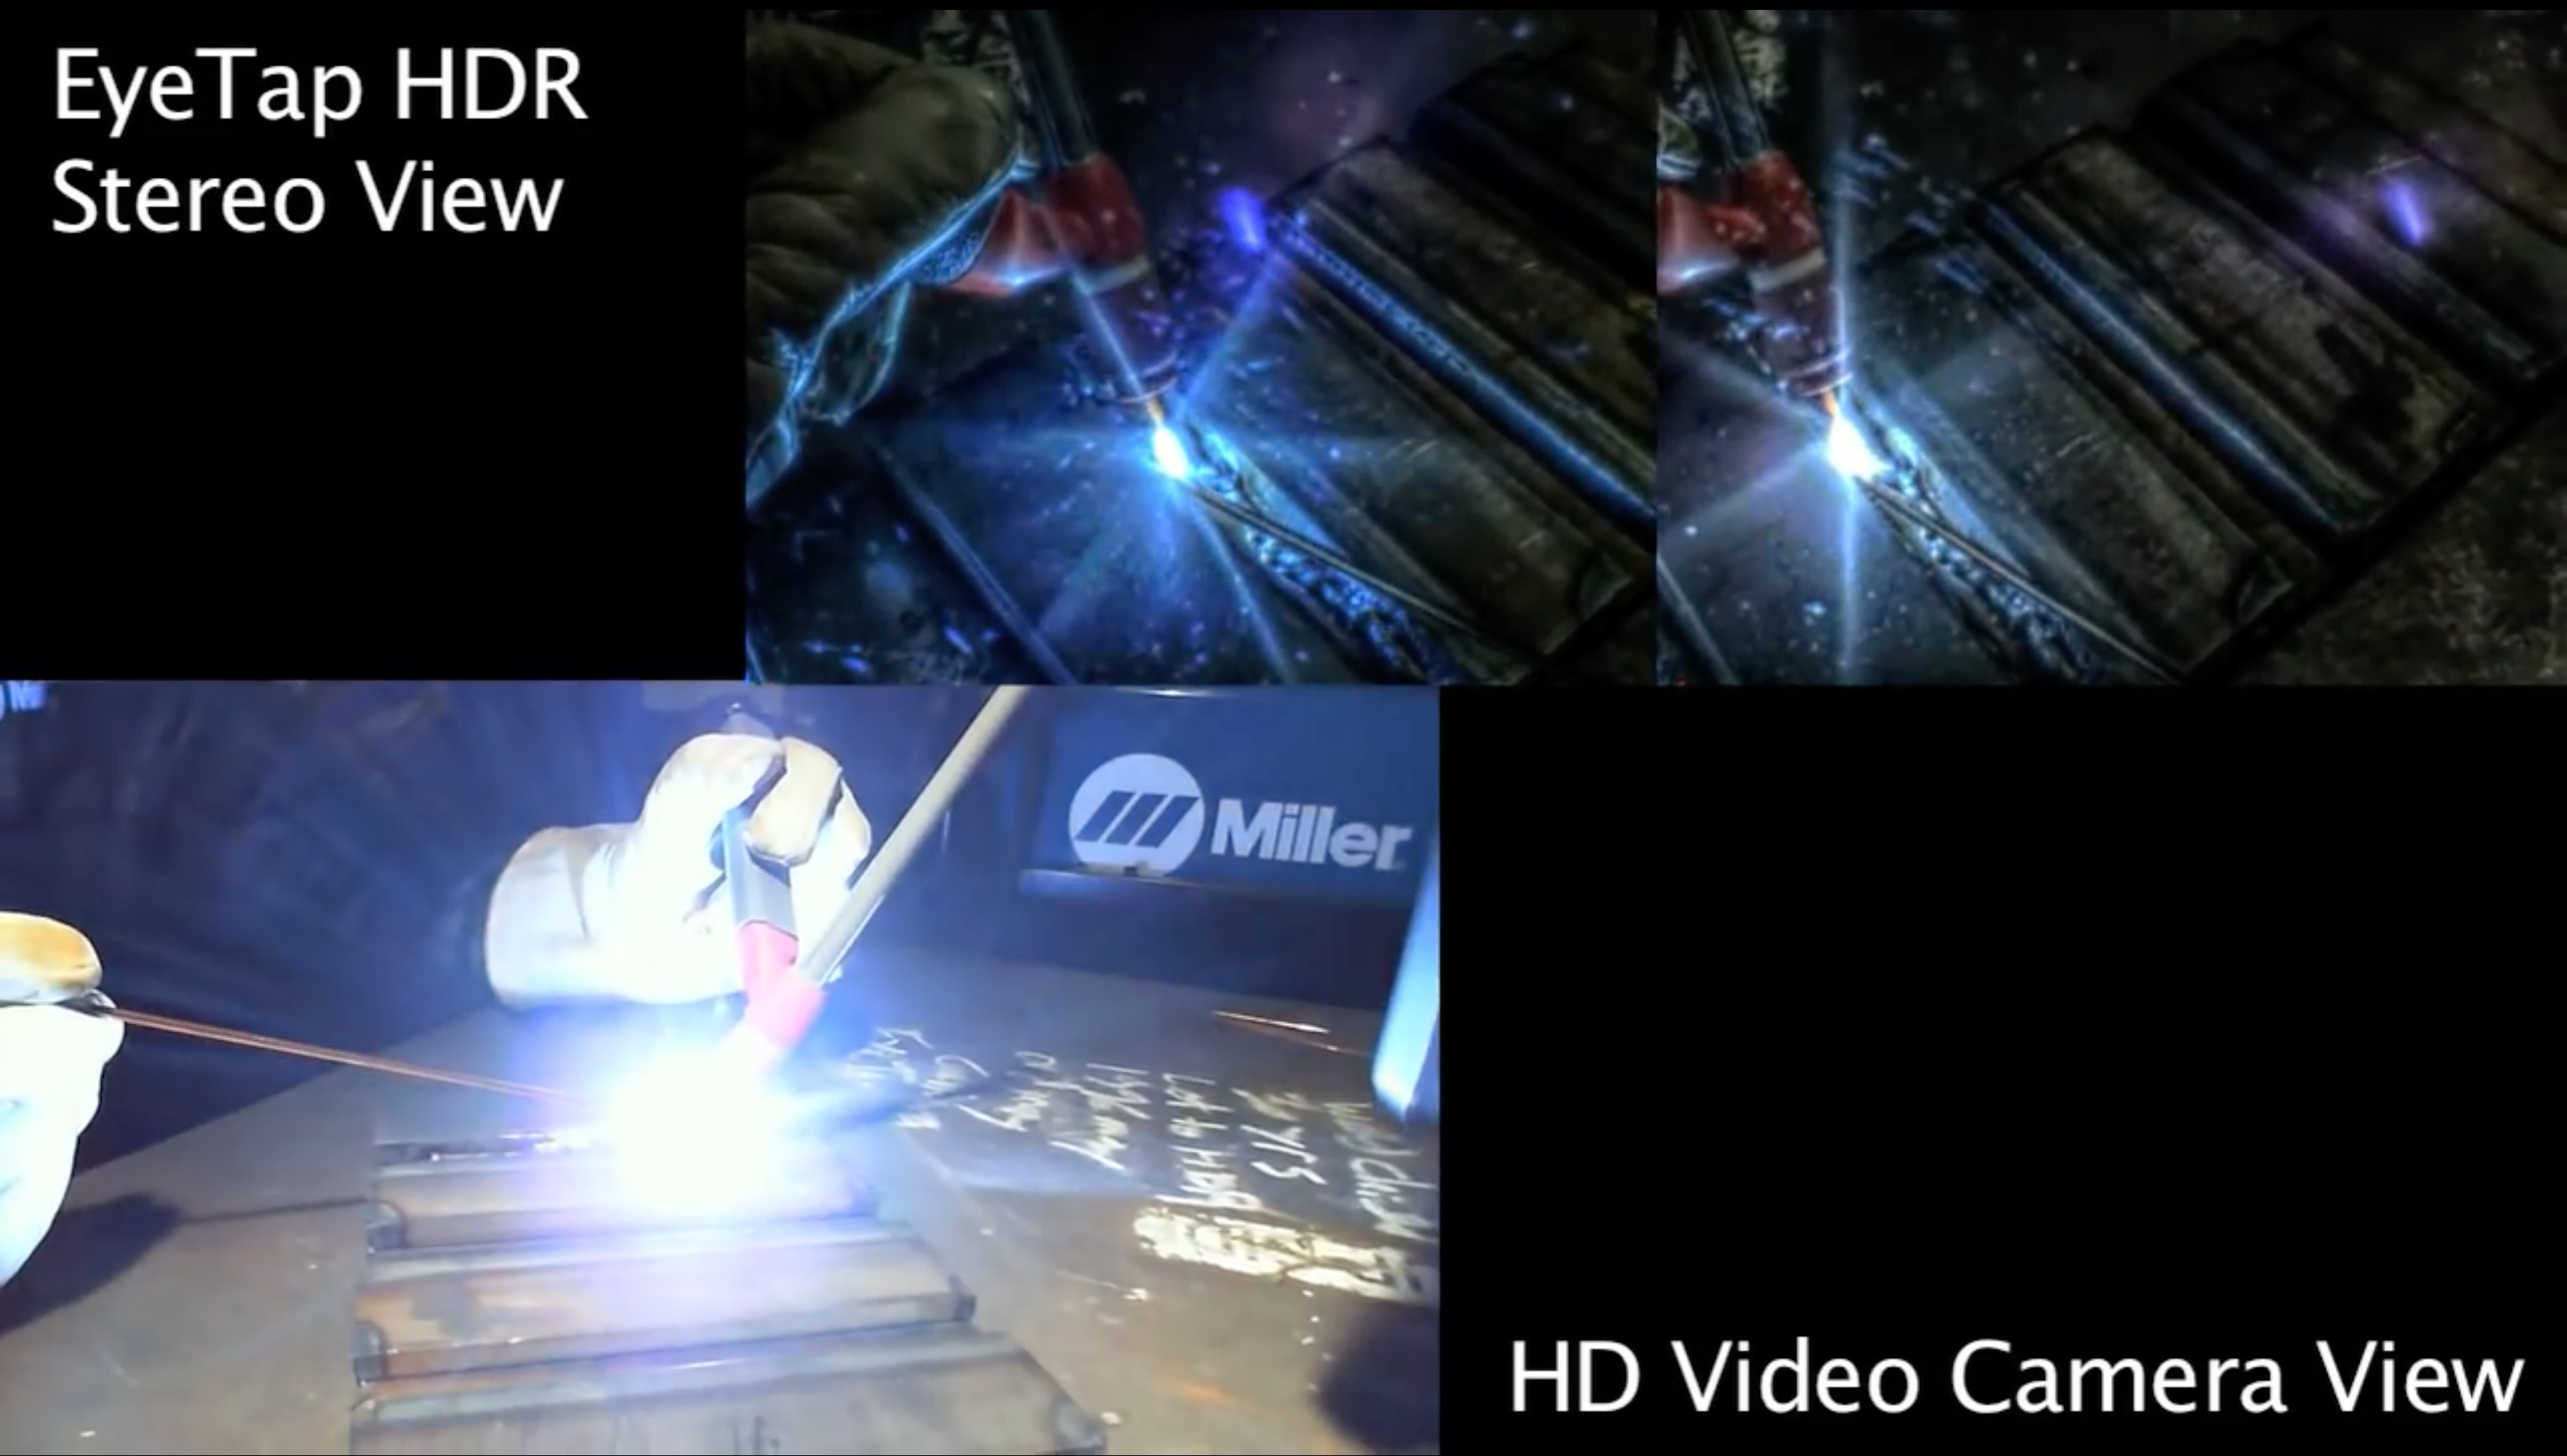
\includegraphics[width=5in]{ch2/diagrams/eyetap_3d_view.png}
% \caption{3D Stereoscopic View of the final HDR rendering. As we can see with ordinary HD video camera the bright light from the TID welding had completely `blinded' the sensor. }
% \label{fig:extreme3dhdr}
%\end{figure}
%
%
%\section{Conclusions and Discussion}
%We demonstrated the feasibility of using hardware to construct HDR video in realtime.  Our approach is parallelizable, and suitable for implementation on GPUs or FPGAs. To test our system, we have applied to TIG welding where extreme dynamic range scene is presented and also worn our seeing devices in our daily life.
%
%Similar to other HDR system which uses alternating exposures, image misalignment between the adjacent frames would product unpleasant ghosting artifacts. Numerous solutions have been proposed to address the image alignments between the consecutive frames. However, these solutions are computationally intense and not yet suitable for real-time usages. Alternatively, we can address this issue by optics which allows us to capture at the same instance, and thus our work in HDR video would be fully benefited from such hardware. 
%

\chapter{Real-time 3D HDR video for EyeTap based on FPGAs and GPUs}
\label{realtimehdrfpgas}

This chapter presents the implementation of a real-time High Dynamic Range (HDR) video 
processing framework in the context of a seeing aid designed for task-specific use (e.g., electric arc 
welding). It can also be built into regular eyeglasses to help people see better in their everyday lives.

The prototype described in this chapter consists of an EyeTap Digital Eye Glass welding helmet and 
a wearable or mobile computer on which a set of image processing algorithms are implemented to 
enable real-time HDR image processing together with applications such as augmented 
reality~\cite{feiner1997touring,starner1997augmented}, mediated reality~\cite{mann1994mediated}, 
and aug-mediated reality~\cite{mannaaai361}. 

The FPGA-based HDR video system runs in real-time and processes 120 frames per second, in 
groups of three frames or four frames (e.g., a set of four differently exposed images captured every 
thirtieth of a second). The processing method, for implementation on Field Programmable Gate 
Arrays (FPGAs), achieves real-time performance for creating HDR video using our novel compositing 
methods, and runs on a miniature self-contained, battery-operated, head-worn circuit board, without 
the need for a host computer.  The result is essentially a stand-alone, miniaturized hardware HDR 
camera system that could be built into smaller eyeglass frames for use in various wearable 
computing and mediated/ aug-mediated reality applications, as well as to help people see better in 
their everyday lives.

Secondly, a highly parallelizable and computationally efficient HDR image compositing, 
reconstruction, and spatio-tonal mapping algorithm for processing HDR video for GPUs is presented 
in this chapter. The algorithms described in this chapter can run on commodity hardware, CPUs and 
GPUs, with the EyeTap Digital Eye Glass electronic seeing aid, and is designed for use in our 
everyday lives. By utilizing the GPU architecture, this approach can be widely adopted for research 
and create customized ``prescription" for various use cases, such as different dynamic range setting 
or different sensor architecture. To validate the robustness of the algorithms, the system was tested 
in extreme dynamic range situations, such as electric arc welding, or looking directly into the sun. 
The GPU-based system also runs in real-time, and requires no user intervention, or fine-tuning of 
parameters after a one-time calibration, even under a wide variety of very difficult lighting conditions 
(e.g., electric arc welding, including detailed inspection of the arc, weld puddle, and shielding gas in 
tungsten inert gas [TIG] welding). The approach can render video with a resolution of 1920x1080 
pixels at interactive and sustainable frame rates of 60 frames per second with GPU acceleration.


The work presented in this chapter was peer reviewed and published in the following list of 
conferences: 

\begin{itemize}
\item
Raymond Chun Hing Lo, Steve Mann, Jason Huang, Valmiki Rampersad, and Tao Ai. High dynamic 
range (HDR) video image processing for digital glass. In Proceedings of the 20th ACM international 
conference on Multimedia, pages 1477--1480. ACM, 2012.
\cite{lo2012high}
\item
S. Mann, R. Lo, J. Huang, V. Rampersad, and R. Janzen. HDRchitecture: Real-time stereoscopic 
HDR imaging for extreme dynamic range. In ACM SIGGRAPH 2012 Emerging Technologies, page 
11. ACM, 2012
\cite{mann2012hdrchitecture}
\item
S. Mann, R.C.H. Lo, K. Ovtcharov, S. Gu, D. Dai, C. Ngan, and T. Ai. Realtime HDR (high dynamic 
range) Video for EyeTap Wearable Computers, FPGA-based Seeing Aids, and Electric Eyeglasses. 
image, 1(2):3--4, 2012.
\cite{mann2012realtime}
\end{itemize}

\section{Introduction}

Existing cameras can only sense a limited dynamic range at any single given exposure, much less 
than the human eye. One method to overcome this limit is to combine differently exposed images of 
the same subject matter, resulting in a High Dynamic Range or HDR image \cite{mannist, comparam,
  robertson2003estimation, kang2003high}. 
  
The history of HDR digital photography goes back almost two decades, as Robertson et al.\ 
stated\cite{robertson2003estimation}:
\begin{quote}
  ``The first report of digitally combining multiple pictures of the
  same scene to improve dynamic range appears to be
  Mann\cite{mannist}''
\end{quote}

With HDR, it is now possible for cameras to match, or even exceed the dynamic range of the human 
eye by orders of magnitudes. The most common method of compositing multiple Low Dynamic 
Range (LDR) images to form an HDR image is to first estimate the photoquantity\footnote{This 
quantity is often incorrectly called radiance or luminance. It is neither, since the spectral response of 
a camera is not flat (i.e. the quantity is not radiance), nor the same as the human eye (i.e. the 
quantity is not luminance).}  by independently transforming each of the input images to an estimate of 
the photoquantity, and then combining these estimates using a weighted sum over a certainty 
function~\cite{mannist, mannwyckofftr, comparam, intelligentimageprocessing}.
This estimate may then (optionally) be transformed via a spatio-tonal mapping (``spatio-tonal 
mappings'' are mappings that depend neither on space or tone alone) for viewing on an LDR display 
(8 bits per channel).  More complex methods relying on per-pixel non-linear optimization are difficult 
to apply directly in a real-time context~\cite{pal2004probability, kang2003high, granados2010optimal} 
as they do not perform linearly and do not have a deterministic runtime.

This chapter presents a real-time wearable HDR seeing aid designed for task specific use 
(specifically, electric arc welding). The prototype EyeTap welding helmet is shown in 
Fig.~\ref{fig:mannvis}, and is known in the welding community as the ``MannVis'' (Mann Vision) 
system.
\begin{figure}[t]
  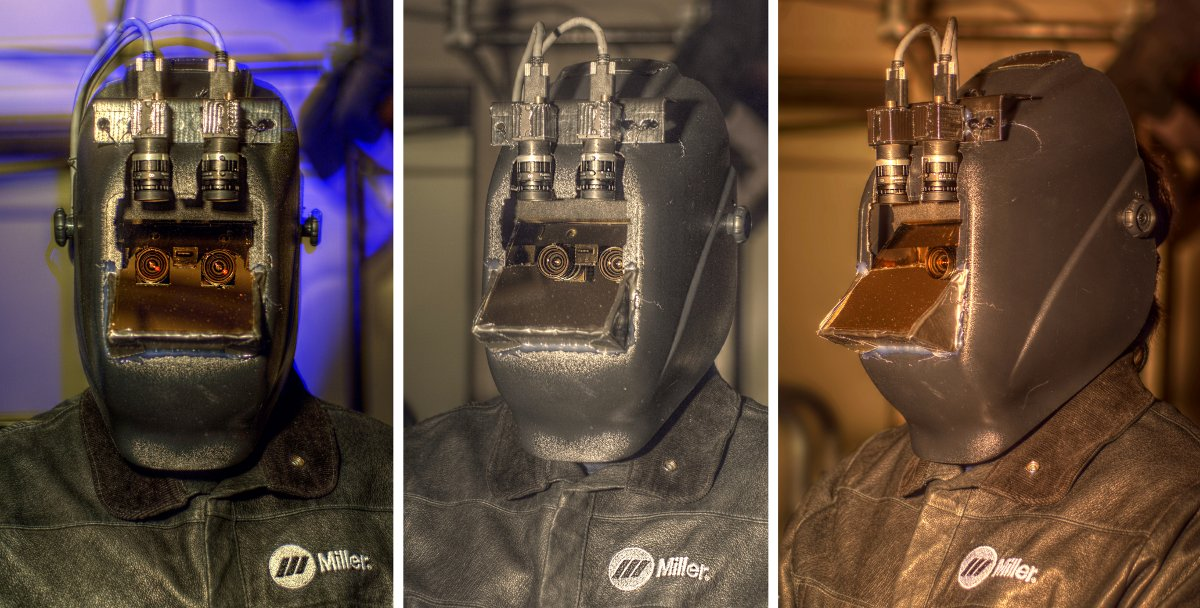
\includegraphics[width=15cm]{ch3/diagrams/cyborg_welding_helmet_2011_02_18_09_53_54_39004100_lowres.jpg}
 \caption{The ``MannVis welding helmet'' implements the EyeTap
   principle which causes each eye to, in effect, function as if the
   eye itself were both a camera and display.  Rays of eyeward-bound
   light are diverted into a pair of downward-pointing cameras by way
   of a diverter, formed from a gold film deposited on the front of a
   welding shade, mounted at a 45-degree angle in the helmet.  The
   shade slides into a slot built into the helmet, so that it can be
   easily replaced if it becomes damaged from splatter, slag, or
   sparks.  The images from the camera are processed for display to an
   audience on a 3D TV, or a live WeldCast$^{TM}$, as well as in the
   wearer's own eyes, where the image is redrawn on the wearer's
   retinas with computer-controlled laser light sources that trace an
   LDR (Low Dynamic Range) image comfortably displaying the more than
   100 million-to-one input dynamic range as a typical 1000:1 output
   dynamic range.  {\bf Note the way in which it appears that the
     wearer has ``glass eyes''.  What we are seeing is a reflection of
     the cameras in the exact position of the wearer's eyes}~\cite{mann2012realtime}. }
 \label{fig:mannvis}
\end{figure}

The real-time video HDR framework, however, has many more far-reaching
applications:
\begin{itemize}
\item as a general-purpose seeing aid, it consists of an EyeTap camera
  system connected to a wearable computer utilizing a set of image
  processing algorithms that improve the wearer's vision through HDR,
  along with mediated and aug-mediated reality;
\item as a drop-in replacement for security cameras, e.g., for general
  purpose surveillance and sousveillance (e.g., inverse surveillance)~\cite{mann2002sousveillance};
\item for general-purpose video cameras both hand-held and
  tripod-mounted.
\end{itemize}

The hardware implementation uses Field Programmable Gate Arrays (FPGAs).  The initial prototype 
includes a low-power (battery-powered) circuit board, which is small enough to fit inside a large
shirt pocket or inside the MannVis welding helmet.

The design is miniaturizable, in the sense that a new circuit board layout can be made to fit into the 
temple side-pieces of eyeglass frames.  The circuit board includes two HDMI camera inputs, one 
being used for the left eye, and the other for the right eye, as well as HDMI outputs fed back to the 
left and right eyes
(head-up displays, EyeTap, or the like), after processing of the video signals.  The current 
implementation runs on a Xilinx Spartan 6, LX45 FPGA, but can be easily adapted to any of a wide 
variety of other FPGAs.

This chapter also presents the state-of-the-art implementation of HDR video processing for extreme 
dynamic range conditions where the scene is relatively static but with high contrast. Unlike previous 
approaches where images are captured with very fine bracketing (e.g., capturing 9 images which are 
one exposure value apart), a scene with a bright light source and dark background (i.e., extreme in 
contrast) is chosen and is captured at 60 fps with 3 different exposures, 4 stops apart. 

%two more examples here
Recently, Michael et al.~\cite{HDRVideoCamera11} proposed a system which captures HDR video 
with an optical arrangement having multiple sensors. One advantage of such a system is its ability to 
simultaneously capture differently exposed images and thus eliminates mis-registration artifacts due 
to motion. Alternatively, modern digital cameras such as the Canon 5D Mark II camera can be 
programmed to capture videos with alternating exposures with a simple modification to the firmware 
(See \textbf{Appendix~\ref{apx:5dIII}}). However, these systems record the videos on flash memory 
and the HDR processing tasks (combining the differently exposed videos and tone mapping) are 
time-consuming offline post-processing tasks that do not run in real-time.  Therefore, such a system 
cannot be used as a real-time seeing aid, nor does the videographer receive immediate visual 
feedback on the recorded HDR videos. 

To address these issues, novel hardware-accelerated algorithms for constructing HDR videos from a 
sequence of alternating exposures, were implemented using GPUs for real-time HDR processing. 
The hardware-accelerated results are useful for seeing aids, as well as being able to shoot videos 
while observing the HDR video result in a viewfinder, display monitor, or other similar outputs. Thus, 
a videographer would be able to compose the shot more effectively while being able to render the 
final result in real-time.

Together with our spatial-tonal mapping algorithm, which is based on a GPU implementation of the 
edge-preserving recursive filter in~\cite{GastalOliveira2011DomainTransform}, real-time (see 
Table~\ref{perf_table}) results that are comparable or better than some of the state-of-the-art tone 
mapping algorithms~\cite{reinhard2002photographic,mantiuk2006perceptual,fattal2002gradient} 
were achieved, especially under extreme lighting conditions such as TIG welding 
(Fig.~\ref{fig:welding_results}).

\section{Background}
 
\subsection{Dynamic range}
Let us begin by defining 2 kinds of dynamic range:
\begin{itemize}
 
 \item 
%%% 
       {\bf Transmitient dynamic range} is the
       dynamic range in signal production.
       For example, the dynamic range of a clarinet is the range from
       quietest sound to loudest sound it can make;
 \item 
 
       {\bf Recipient dynamic range} is a sensed or measured dynamic range,
       such as a sensor's dynamic range.
 
\end{itemize}
 
To the extent that what's between these two is representable as a function, one might call the former 
the {\em dynamic domain} of this function, and the latter its {\em dynamic range}.

One's first encounter with dynamic range is more likely to be the latter than the former, i.e., concern 
for dynamic range (especially its specific quantification in decibels or f-stops) is more likely to arise 
from devices such as sound recorders and photographic cameras than from sound and light sources.

In that sense, we care more about the dynamic range of the human eye or a camera, for example, 
than we do about the dynamic range that could exist philosophically in the {\em transmitient} sense 
(e.g. between bright sunlight and the inside of a coffin in an Egyptian tomb deep underground).

Very few people would ask ``how many dB dynamic range is a clarinet?''.  To answer such an ill-
posed question, do we take the ratio of the loudest note to the silence it produces when sitting on a
desk not being played? Or do we go from the quietest sound it can make to the loudest sound it
can make, regardless of musical integrity?  Or do we take the ratio of undistorted quietest note to 
undistorted loudest note?  The dynamic range would depend on how much distortion we can accept, 
so it becomes very
imprecise in terms of definition.

Let us, therefore, define {\em dynamic range} as follows:
\begin{quote}
  Dynamic range is the ratio
    between the largest and smallest non-negative quantity such
    as magnitude, amplitude, or energy, of
    sound, light, or similar phenomena, for 
    which a small incremental difference in the quantity can still be
    sensed (i.e., the range over which changes in the quantity remain
    discernible).
\end{quote}
Compare with the definition provided in~\cite{tei2011}.
 
\subsection{``Dynamage range''}
 
Let us define an additional concept called ``dynamage range'' as follows:
\begin{quote}
  ``Dynamage range'' is the ratio between the largest quantity
    that will not damage a sensor or device or receiver and the
    smallest non-negative quantity for which changes in the quantity
    remain discernible.
\end{quote}

HDR video was made possible by the invention of cameras that can be overexposed without 
permanent damage.  Unlike old vidicon cameras \cite{Vidiconc95:online} for which the dynamic range 
and dynamage range are roughly equal, modern cameras have a much greater dynamage range 
than their dynamic range.

HDR allows us to increase the dynamic range up to being equal to the dynamage range.


 
\subsection{The EyeTap Principle}
 
The experimental seeing aid system (Fig.~\ref{fig:mannvis}) is constructed with the form factor of a 
standard welding helmet shell, but with two computer-controlled video cameras mounted in a 
binocular configuration facing downwards, pointing toward a welding shade mounted at a
$45^{\circ}$ pitch from the coronal plane.  A gold plating on the welding shade directs the light from 
the front of the wearer toward the cameras. 

Additionally, a computer-controlled stereoscopic display system is built into the helmet, which directs 
light into the wearer's eyes. In this way, the system provides Mediated 
Reality~\cite{intelligentimageprocessing}, a proper superset of Augmented Reality. Augmented reality 
is limited in the sense that it simply adds new matter, but in this case what we really wish is a {\em 
diminished reality}, i.e. to reduce the severity of the contrast ratio locally and selectively such that it 
provides the best possible image to the user. 

The point-of-view of the cameras is the point-of-eye (PoE), such that each camera operates as if it 
were the wearer's own eye. The laser light image forms inside the wearer's own retinas, so as to 
show what is present, but with dynamic range compression when needed. This is called the 
``dynamic range management''. With
dynamic range management, any lighting situation presented to the wearer is managed by the 
computer system to keep the overall lighting in certain ranges.  This is beyond auto-darkening 
eyewear that only manages light levels, because now the contrast, in addition to the light levels 
overall, is managed. 

 
\subsection{Comparametric Equations}\label{sec:comparam}
 
Comparametric equations\cite{comparam} and superposimetric equations~\cite{manders_icip2004} 
are mathematical frameworks for understanding pictures or video of differently exposed or differently
illuminated pictures of otherwise identical subject matter.  This conceptual framework captures the 
general essence of linearity and superposition of light, and in particular, photoquantities, irrespective 
of any non-linearities that might be present in a particular camera system.

In this chapter, the situation where sequential frames of videos, $f_i \in \{ f_1, f_2, f_3, \ldots \} $, are 
captured in rapid succession, with varying exposure levels $k_i$, is considered.  These exposure 
levels are controlled by the wearable computer system to extend the dynamic range, resulting in a 
set of differently exposed video
frames, $f_i = f(k_i q(x,y))$.  This set of pictures is used to estimate the true photoquantity, $q(x,y)$ 
(a spatially varying quantimetric measure of light on the image plane defined by coordinates $x$ and 
$y$).  


% XXX maali: there is nothing in this paper or the implementation
% AFAIK that supports dynamic adaptation to a new camera response
% function

% The first step taken by the wearable computing system is a
% self-calibration step of automatically determining the response
% function(s) of whatever camera(s) happen(s) to be plugged into it.
% This is done by way of automatically solving the comparametric
% equations inherent in each particular camera (every camera has
% associated with it a particular response function, and thus a
% particular comparametric equation that requires solution before
% constructing the HDR pipeline).  

% Following our results in \cite{ali2012ICASSP}, we present here an
% FPGA-based implementation of HDR processing, wherein the HDR
% compositing process is effected using pre-computed \textit{lookup
%   tables} (LUTs), and the tonal mapping for LDR display via an HDMI
% interface is also performed onboard in real-time.

%%%%%%%%%%%%%%%%%%%%
% The problem inherent in solving a comparametric equation may be
% transformed into a problem of solving a differential equation.
% This transformation arises quite obviously from the scaling operators
% commonly used in the study of quantum mechanics, and, specifically,
% quantum field theory.
% Let us proceed with an approach one might find
% in many introductory texts on quantum mechanics
% (see, also, the work of Sophus Lie, the inventor of Lie Algebra):

% In quantum field theory we often use a scaling operator $S_k$,
% and wish to derive an explicit expression for this operator.
% First consider an
% infinitesimally small scaling of the function $f$. Let $\epsilon$ be
% a very small number. We have, up to first order in $\epsilon$
% %
%  
% \begin{equation}
% \label{infsc}
% f((1+\epsilon)q) \approx f(q) + \epsilon \, q
% \frac{\partial}{\partial q} f(q).
% \end{equation}
% %
% By repeated application of the infinitesimal scaling of $q$ we can
% scale $q$ by any amount $e^\Lambda$
% \vspace{-.14in}
% \begin{equation}
% e^{\Lambda} q = \lim_{N \rightarrow \infty}
% \left(1+\frac{\Lambda}{N}\right)^N q.
% \end{equation}
% %
% N-time application of Equation~\ref{infsc} with
% $\epsilon=\frac{\Lambda}{N}$ for $N$ large gives
%  
% \begin{equation}
% f(e^{\Lambda} q) = \lim_{N \rightarrow \infty} \, 
%   \left( 1+ \frac{\Lambda}{N} q \frac{\partial}{\partial q} \right) ^N f(q),  \,\, \\
% %&& \mbox{so that as $N \rightarrow \infty $ we get} \\ 
% %f(e^{\Lambda} q) 
% = \exp \left[ \Lambda q \frac{\partial}{\partial q} \right] f(q) .
% \end{equation} 
% %
% Choosing $\Lambda=\log (k)$ we scale $q$ by $k$ and thus define the
% scaling operator $S_k$ as
% %
% \vspace{-.12in}
% \begin{equation}
% S_k=\exp \left[ \log (k) q \frac{\partial}{\partial q} \right].
% \end{equation} 
% %
% The exponential here is defined as the formal series 
% %
%  
% \begin{equation}
% \exp \left[ 
%     \log (k) q \frac{\partial}{\partial q} 
%   \right] 
% = 
% \sum_{n=0}^\infty \, \frac{(\log(k))^n }{n !} 
%      \left( q \frac{\partial}{\partial q} \right)^n.
% \end{equation}
% %
% Each differential operator in this series acts on every term to the
% right of it.  The inverse of the scaling operator is then
%  
% \begin{equation}
%   (S_k)^{-1} = 
%   S_{1/k} = 
%   \exp \left[ -\log (k) q \frac{\partial}{\partial q} \right].
% \end{equation}
% Now given $g(k,f)$ we can write down $f(q)$ formally as
% %
%  
% \begin{equation}
% \label{formaleq}
% f(q) = S_{1/k} g(k,f(q)).
% \end{equation}
% %
% Although this is not a convenient formulation for explicit
% computation of $f(q)$, it opens the possibility for further analysis
% of the general comparametric problem using the machinery of the
% well-known operators arising in quantum field theory.  Since
% (\ref{formaleq}) holds for any value of $k$, we can take $k$ close
% to one i.e. $k=1+\epsilon$ for $\epsilon \approx 0$ and we see that
% %
%  
% \begin{equation}
%   f(q) =\exp \left[ 
%     - \log (1+\epsilon) \, q \frac{\partial}{\partial q}
%   \right] g(1+\epsilon,f).
% \end{equation}
% %
% If we expand this up to first order in $\epsilon$ we find
% %
%  
% \begin{equation}
% f(q) = \left.\left[1- \epsilon \, q \, \frac{\partial}{\partial q}\right] \left[g(1,f) + 
% \epsilon \frac{\partial g(k,f)}{\partial k}\right]\right|_{k=1}.
% \end{equation}
% %
% Using the identity $f=g(1,f)$ we end up with an ordinary differential equation
% %
%  
% \begin{equation}
% \frac{df}{dq}= \left. \frac{1}{q} \, \frac{\partial g(k,f)}{\partial k}\right|_{k=1}.
% \end{equation}
% %
% from which we can obtain $f(q)$.



\section{Real-time HDR Video Processing}
\label{realtime_hdr}

In this section, a novel HDR image composition method, optimized for FPGA hardware 
implementation of electric eyeglasses, is discussed. This method, advancing upon the results 
in~\cite{mannist,robertson2003estimation,ali2012ICASSP}, is specifically designed for direct 
hardware implementation, as opposed to assuming the availability of a multicore CPU or GPU.  
Additionally, the implementation on how this method can be extended
to three or more images in extreme dynamic range cases using simple
binary operators is presented.
 
\subsection{Mathematical Notation}

Let $f$ represent the \textit{camera response
  function} (CRF), where $f$ in a scalar context is a \textit{tonal
  value}, and in a matrix context $f$ is a \textit{tonal image} (e.g.\
a picture from a camera).  A tonal value $f$ to vary
linearly with pixel value is considered but on the unit interval, and given an
$n$-bit pixel value $v$ returned from a physical camera, $f_i =
(v+0.5)/2^n$ is used, where $N$ images, $i\in\{1,\ldots,N\}$, each
image with exposure $k_i$, are captured. The subscript indicates it is the $i$-th in
a \textit{Wyckoff set}\cite{comparam}, i.e.\ a set of images differing
only in exposure, and by convention $k_{i}<k_{i+1} \;\forall\; i<N$.
$f^{-1}$ is used as the mathematical inverse of $f$ if it has only one
argument, and otherwise as a joint estimator\footnote{A ``joint
  estimator'' is used here in the sense that each photoquantity
  estimate depends simultaneously on multiple measurements.} of the
photoquantity $\hat{q}$.

 
\subsection{Direct Lookup method for combining
  exposures} \label{comp_2_lut}
 
For the case of compositing two images with 8-bit color depth per
channel, a 256$\times$256$\times$3 lookup table (LUT) can be derived for each camera.
The LUT needs to be computed only once each time a new camera is plugged
in for the first time.

 
\subsubsection{Constructing the inverse comparametric LUT}

The inverse comparametric lookup table (CLUT) is a composition of a set
of operations for creating HDR images from an alternating exposure
set.  To construct this look-up table, the response
function of the camera along with its certainty function is estimated using the
method described in Section~\ref{sec:comparam}.

An estimate, $\hat{q}$, of the photoquantity is computed from the
pixel (tonal) values $f_1$ and $f_2$.  This can be by a weighted average
with the certainty function $w$ and with the response function $f$ of
the camera.  To speed up the process (for real-time video), this may be
determined using conditional statements in handling the saturated regions:

\begin{equation}\label{joint_est}
\begin{split}
  \hat{q}=&f^{-1}_{\Delta EV}(f_1, f_2) \\
  =&\begin{cases}
    q_{max}&\text{if $f_1 > \beta$}, \\
    q_{min}&\text{if $f_2 < \alpha$ }, \\
    \frac{f^{-1}(f_1) \cdot w(f_1)+f^{-1}(f_2) \cdot w(f_2) \
      / 2^{\Delta EV}}{w(f_1)+w(f_2)}& \text{otherwise},\\
\end{cases}
\end{split}
\end{equation}
where $\beta$ and $\alpha$ are the saturation parameters of the camera
(Typical values are $\beta$ = 250 and $\alpha=5$.)  and $\Delta EV$ is
the exposure difference between $f_1$ and $f_2$, and $q_{max}$ and
$q_{min}$ are the estimated $\hat{q}$ values at the saturation points,
$f^{-1}(\beta)$ and $f^{-1}(\alpha)$, respectively.

In the prototype, the camera is configured to capture images that are
4 stops apart (i.e., one image has an exposure time that is $2^4=16$
times longer or shorter than the other or has the ISO value 16 times larger or smaller than the other).

Once $\hat{q}$ from the image set is estimated, dynamic range compression (tone mapping) is 
applied for visualization on an LDR display.
Empirically, the following function can provide
adequate dynamic range compression and works well for general high
dynamic range scenes.  

\begin{equation}\label{compressor}
 \hat{q}_{c}=c(\hat{q})=
 r\cdot\hat{q}^{1/k}+d	\\
\end{equation}
where $r$, $k$, and $d$ can be used to adjust ``contrast'' and
``brightness'' of the output image (e.g., k=5, d=-1.0, and r=1.8).

\begin{figure}
\center
 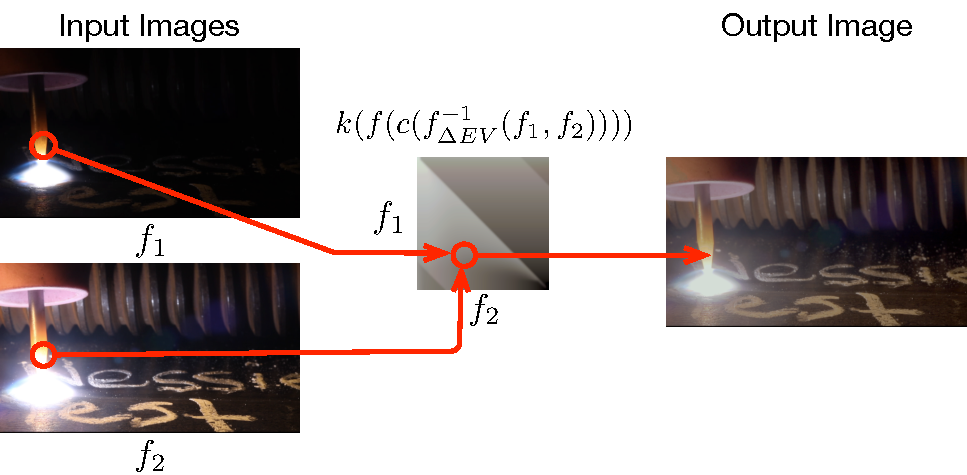
\includegraphics[width=13cm]{ch3/diagrams/direct_lut_method.pdf}
 \caption{\textbf{The composite direct lookup method.} The lookup table $Q_f$ (center) is the value of 
the composition of functions $ k \circ f \circ c \circ f^{-1}_{\Delta EV} $, where  $ f^{-1}_{\Delta EV} $ is 
the joint photoquantity estimator function for two exposures $ {\Delta EV} $ apart, $c$ is the dynamic 
range compression function, $f$ is the CRF, and $k$ is the contrast enhancement function. The value 
of $Q_f (f_1, f_2)$ is evaluated at all possible values of $f_1$ and $f_2$ to create the lookup table 
shown here. This method can be extended to 12-bit or 14-bit images by applying linear interpolation 
to obtain intermediate values from an arbitrarily-sized table~\cite{mann2012realtime}.}
 \label{cdlut}
\end{figure}

After a new range-compressed $\hat{q_c}$ is obtained, the output value is estimated by applying the 
CRF to 
$\hat{q_c}$. Since the equation of the CRF may not have a closed form
solution, a nearest neighbor search is applied which
minimizes the absolute distance between $\hat{q_c}$ and $q$
from the response function of the camera.
\begin{equation}
\begin{aligned}
Q = & \underset{z\in \mathbb{N}}{\operatorname{argmin}}{(|f^{-1}(z)-\hat{q_c}|)} \\
\end{aligned}
\label{opt_min}
\end{equation}
Notice that now Q is a quantized output which maps to the range
[0-255] for LDR displays. To further adjust the contrast level of the
image, an additional tonal adjustment function $k$ is applied to
the final result.  
% 
\begin{equation}\label{contrast_enhancement}
 Q_f=k(Q)
\end{equation}
where k can be a simple look-up table for the desired color profile.


% \newcommand{\CDLUT}{\mbox{CDLUT}} 
\newcommand{\CLUT}{\mbox{\textsc{Clut}}}

Lastly, the above function is applied to obtain a solution for all
possible values of $f_1$ and $f_2$. The result
is shown in Fig.~\ref{cdlut}.
\begin{equation}
  \label{combined_function}
  Q_f = k(f(c(f^{-1}_{\Delta EV}(f_1,f_2)))) = \CLUT{}(f_1, f_2)
\end{equation}

\subsection{Compositing 3 or more exposures} \label{comp3_set} 

For the case of constructing HDR images from 3 or more images, an intermediate estimation of the 
photographic quantities
$\hat{q_i}$ is computed using Eq.~\ref{joint_est}. Since the images only differ in
exposures (i.e., 4 stops in our case), the same LUT which precomputed
 $\hat{q_i}$ can be applied to the image pairs at no additional
computational cost.
\begin{equation}
\hat{q_i}=f^{-1}_{\Delta EV}(f_i, f_{i+1}), i \in \{1,..,N\}
\end{equation}
\begin{equation}
\hat{w_i}=\max(w(f_i), w(f_{i+1})), i \in \{1,..,N\}
\end{equation}
Then, the individual photoquantities $\hat{q_i}$ are combined with the
certainty values $w_i$ computed from the last step
\begin{equation}
\hat{q}=g(q_i, q_{i+1}, ... , q_{N-1}, w_i, w_{i+1},...,w_{N-1})
\end{equation}
to create our final estimate of $\hat{q}$.  For the case of 3 images,
the function $g$ can be implemented as a simple weighted average of 
 $q_1$ and $q_2$ with respect to the certainty values $w_1$ and
$w_2$:
 
\begin{equation}
\begin{split}
  \hat{q} = g(\hat{q_1}, \hat{q_2}, w_1, w_2) = \frac{\hat{q_1} \cdot
    w_1 + \hat{q_2} \cdot w_2 / 2^{\Delta EV}}{w_1+w_2}
\end{split}
\end{equation}
One advantage of the proposed algorithm is that the problem is reduced
into sub-steps that can be easily optimized for a specific scenario and
can provide a significant speed-up.

\begin{figure}
\center
  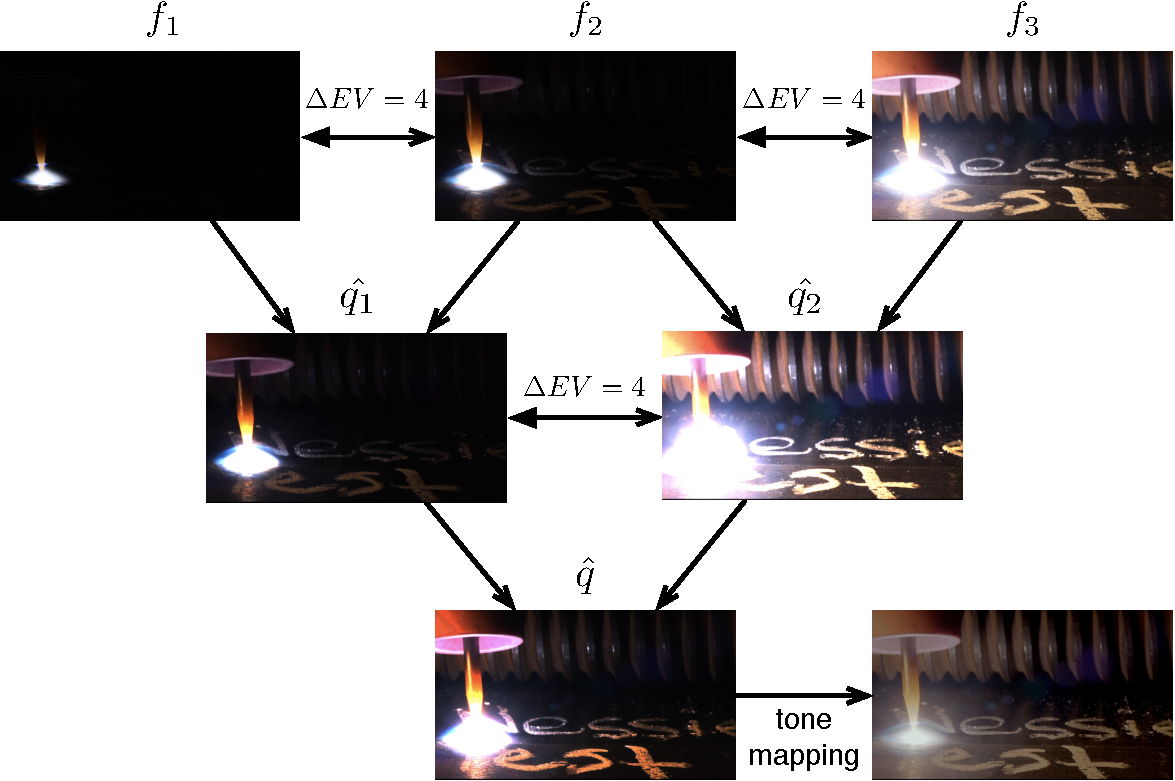
\includegraphics[width=13cm]{ch3/diagrams/3_composite_LUT.pdf}
  \caption{Composition of HDR images using our pairwise approach for
    combining three LDR images, $f_1$, $f_2$, and $f_3$. The final
    estimate of the photoquantity $\hat{q}$ then undergoes
    tonemapping~\cite{mann2012realtime}.  }
  \label{composite3}
\end{figure}
With an image set of 3 differently exposed images, the dynamic range is extended by another 4 
stops, a total of 8 stops of additional range.  The compressor function in Eq.~\ref{compressor},
however, is no longer suitable for such a wide dynamic
range. In particular, the contrast of the image was poor and
there was a lack of saturation.  A piecewise function which places
emphasis on the highlights is used.  Despite the simplicity of our
piecewise dynamic range compressor, it provides natural looking
results without accentuating noise and other artifacts: % 
\begin{equation}\label{compressor_new}
  \hat{q_c}=c(\hat{q})=
\begin{cases}
  r\cdot (s \cdot \hat{q})^{1/k}+d& \text{if $\hat{q} \le 1/s$},	\\
  r\cdot (s \cdot \hat{q})^{1/({\gamma \cdot k)}}+d& \text{if $\hat{q}
    > 1/s$}.
\end{cases}
\end{equation}
In the proposed setup, $r=1.8$, $k=4$, $d=-1.2$,
$\gamma=1.5$, $s=140$, and $\hat{q}$ is normalized to [0,1].

Finally, the range-compressed image $\hat{q_c}$ is mapped to the LDR display using 
Eq.~\ref{opt_min} and \ref{contrast_enhancement}. To enhance the local contrast of the final image, 
an unsharp mask is applied to the final image. The final and intermediate results of our algorithm are 
shown in Figure~\ref{composite3}.


\subsection{Exposure pruning for further speedup}
The composition technique introduced in Section~\ref{comp3_set} can be
simplified further by computing multiple LUTs in extreme dynamic range
scenarios.  Under these extreme conditions, e.g., compositing three
images that are 4 stops apart (i.e., $\Delta EV=4$), the exposure
difference between the $f_1$ and $f_3$ is a full 8 stops, ($\Delta
EV=8$).  Since there is very little overlap between lightest and
darkest image, a further speedup can be obtained
by pruning image pairs and discarding the exposures that provide very little or no additional
scene information.  In the case of 3 exposures that are 4 stops apart,
the following conditional statement is used to select the
candidate image pair that would generate our final result using only
LUTs:
\begin{equation}\label{selection_mode}
  Q_f=
  \begin{cases}
    \CLUT(f_2,f_3) & \text{if $f_3 \ge \beta$},         \\
    \CLUT(f_1,f_2) & \text{if $f_1 \ge \alpha$ and $f_3 < \beta$} ,	\\
    0 &\text{otherwise},
  \end{cases}
\end{equation}
where \CLUT{} is the lookup table generated based on
Eq.~\ref{combined_function} with the exposure compensation (i.e.,
multiplying the $\hat{q}$ in Eq.~\ref{joint_est} by $2^{\Delta EV}$)
on $\CLUT(f_1, f_2)$, and $\beta=50$ and $\alpha=20$ are set. Fig.~\ref{3_direct_lut} shows the 
results using this approach.

Furthermore, if the images are also sorted from darkest
to lightest, the two LUTs presented in Eq.~\ref{selection_mode} can be
further compressed into a single LUT with the assumption that the
camera response is monotonic (i.e., $f_1<f_2<f_3$).  Thus, the values
in the upper-triangular (i.e., $f_1>f_2$) part of the LUT can be
replaced by the values from the other LUT.
\begin{figure}
\center
  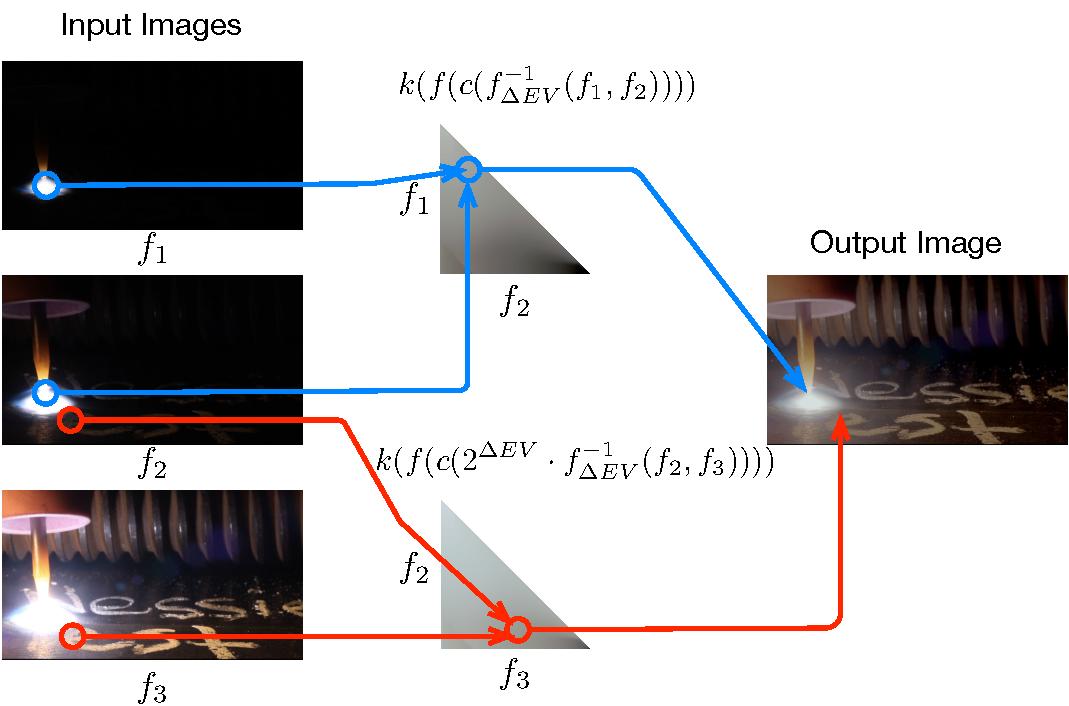
\includegraphics[width=13cm]{ch3/diagrams/3_direct_lut.pdf}
  \caption{Composition of HDR images using a double-LUT approach for
    combining three LDR images, $f_1$, $f_2$, $f_3$~\cite{mann2012realtime}.  }
  \label{3_direct_lut}
\end{figure}

% One disadvantage of this approach is that we might see artifacts if
% we applled extreme local contrast enhancement because we are limited
% to 8-bit data.  But the performance and simplicity (i.e. speed up)
% may

%\begin{algorithm}[]
%\SetAlgoLined
%\KwData{N images 8 bits}
%\KwResult{HDR image 8 bits}
%initialization\;
%\While{not at end of this document}{
%read current\;
%\eIf{understand}{
%go to next section\;
%current section becomes this one\;
%}{
%go back to the beginning of current section\;
%}
%}
%\caption{HDR algorithm}
%\end{algorithm}


%discuss the hdr pipeline and our own algorithm for compressing the
% images efficiently over LUTs

%\begin{figure}
%\label{fig:typical_hdr_pipeline}
%\centering
%\includegraphics[width=3.2in]{ch3/siggraph2010_diagrams/data_flow.pdf}
%%\epsfig{file=ch3/siggraph2010_diagrams/HDRchitecture.pdf}
%\caption{A typical HDR video pipeline.}
%\end{figure}



%Figure \ref{fig:typical_hdr_pipeline} shows a typical HDR imaging
% pipeline.  One key contribution of this paper is the use of various
% parallelization and optimization techniques to obtain a real-time,
% interactive, frame rate. For instance, operations such as image
% blending and light space conversion, are highly parallelizable and
% was offloaded to the GPU, thus allowing the CPU to perform other
% operations, such as tone mapping.
%\begin{figure}
%\centering
%
%%\includegraphics[width=1.07in]{ch3/siggraph2010_diagrams/raw_images/weld_picture/
%3_hdr_canon50d.jpg}
%%\includegraphics[width=1.07in]{ch3/ch3/siggraph2010_diagrams/raw_images/weld_picture/
%2_hdr_canon50d.jpg}
%%\includegraphics[width=1.07in]{ch3/siggraph2010_diagrams/raw_images/weld_picture/
%1_hdr_canon50d.jpg}
%%\newline \newline
%%\includegraphics[width=0.8in]{ch3/siggraph2010_diagrams/raw_images/test_80_1038.jpg}
%%\includegraphics[width=0.8in]{ch3/siggraph2010_diagrams/raw_images/test_80_1039.jpg}
%%\includegraphics[width=0.8in]{ch3/siggraph2010_diagrams/raw_images/test_80_1040.jpg}
%%\includegraphics[width=0.8in]{ch3/siggraph2010_diagrams/raw_images/test_80_1041.jpg}
%%\newline \newline
%\includegraphics[height=1.06in]{ch3/siggraph2010_diagrams/raw_images/welding_hd.jpg}
%\includegraphics[height=1.06in]{ch3/siggraph2010_diagrams/raw_images/output0259.png}
%
%\caption{Two instances of the real-time processed HDR images captured
% from our wearable and standalone system by altering the exposures
% between each frame.}
%\label{final_result}
%\end{figure}


%\section{Code Parallelization \\ and Optimization}

%Another key contribution of this work is the use of various optimization techniques to obtain a real-
%time, interactive, frame rate.

%\subsection{GPGPU}
%To obtain an interactive frame rate, the HDR creation process was
% parallelized across the GPUs and the multi-core
% processor\footnote{Nvidia Geforce GTX 460 and Intel
% Core\texttrademark i7-920 Processor}. The HDR video early work by
% Kang \cite{kang2003high} was running at 0.1 frame per second which
% makes the system impractical for real-time usage. Our
% parallelization approach, distributing the tasks across the GPU and
% multi-core processors has provided an interactive frame rate at 25
% frame per second with a single camera setup or with a linear runtime
% tone mapping algorithm \cite{reinhard2002photographic}.
%
%Once we have converted the images to lightspace and recovered the
%radiance map of the scene, the high dynamic photos needed to be
%compressed into a LDR display (usually 8 bits) for viewing. There are
%several tone mapping algorithms we have implemented
%\cite{reinhard2002photographic, mantiuk2006perceptual} .
%
%\begin{figure}
%\label{fig:hdr_pipeline}
%\centering
%\includegraphics[width=3.5in]{ch3/siggraph2010_diagrams/hdr_pipeling_short.pdf}
%%\epsfig{file=ch3/siggraph2010_diagrams/HDRchitecture.pdf}
%\caption{This figure illustrates one of the acceleration schemes used
% in our system. The General Purpose Graphical Processing Unit (GPGPU)
% sequentially creates HDR frames using our precomputed look-up-tables
% and methods proposed in this paper. After a HDR frame is created,
% the main thread passes it to a free tone mapping thread which runs
% on a single CPU. As seen, multiple instances of the tone mapping run
% simultaneously. This pipeline configuration was chosen because: 1)
% the HDR creation is a per pixel operation, which makes it
% parallelizable on the GPGPU. 2) the tone mapping operator involves
% solving optimization problems that may not run efficiently on GPU,
% thus the multiple instances of the the tone mapping are run on the
% CPU instead. A more efficient and parallalizable tone mapping is
% also proposed in this paper to allow for real-time implementation,
% in a trade off for less dramatic tone and detail enhancements.}
%\end{figure}
%
%
%Due to high data dependencies and underlying complexity in the tone
% mapping algorithm \cite{mantiuk2006perceptual}, the tone mapping
% algorithm itself was parallelized at a higher level using pipeline
% technique. Each instance of the tone mapping algorithm was run on
% each CPU core, which provides us 8 instances of the tone mapping
% algorithm. Therefore, as shown in Figure \ref{fig:hdr_pipeline},
% while the GPU creates 8 HDR frames, the CPU is tone mapping the
% previous HDR frames.
%\end{document}  % This is where a 'short' article might terminate


\section{Real-time FPGA-based HDR Video}
%the ability to be portable and battery operated becomes important. 

In order for real-time HDR processing to be practical as a wearable device, a 45nm
low-power Spartan-6 LX45 FPGA
device\footnote{http://www.xilinx.com/products/silicon-devices/fpga/spartan-6/lx.htm}
was selected for its low power consumption and portability.  The board
contains two input HDMI ports used for receiving the baseband HD video
(720p@60fps) and two output HDMI ports used for transmitting the
processed HDR video frames. It also contains 128MB of DDR2 SDRAM
(Micron MT47H64M16-25E, 16-bit data width), used for storing video
frames. It runs at 625MHz in order to meet the real-time processing
requirements. Additionally, BlockRam (BRAM) is used as line buffers
and to store the LUTs. However, it is limited to a capacity of 2.1Mbits
(116 x 18,432).  Due to resource constraints for wearable applications, a focus on reducing
complexity guided us to invent novel approaches to HDR video processing.  Much of
the processing is pre-computed and stored in LUTs to
reduce complexity using the methods discussed in
Section~\ref{realtime_hdr}.  Each pixel sample contains an 8-bit RGB
colour component totalling 24 bits per pixel.  Each lookup table is
addressed by a color channel of two differently exposed frames.  A
total of 16 bits is used for addressing into the LUT totalling
65536 entries.  For an 8-bit wide sample output, the BRAM was configured
as 8-bit wide x 2048-deep which resulted in 32 BRAMs utilized per
color channel for a total of 96 (out of 116) BRAMs utilized.

Efficient on-chip memory utilization is the key to the LUT implementation
technique, as it directly limits scalability beyond 2 frames. The
number of BRAMs required can be reduced by utilizing the fact that
only half of the data in one square LUT is valid, since each pair of
frames has one's pixels always greater than the other's. This
technique is used in 3-frame implementation using the LUTs as
described in Section 3.4.

\begin{figure}
\center
\centering{
  \includegraphics[width=13cm]{ch3/diagrams/hdr_fpga_vertical.pdf}
 }
 \caption { Block diagram of the real-time HDR video implementation
   using a Spartan-6 LX45 FPGA.  Data is received over HDMI and stored
   in line memory.  The frames are stored in external memory and
   concurrently read back line-by-line.  A direct lookup is performed
   on incoming pixel data and the result is sent through an HDMI
   transmitter~\cite{mann2012realtime}. }
 \label{fig:fpgahdr}
\end{figure}

A variety of different cameras are used in the prototypes, some with
Firewire interface, some with USB interface, and some with HDMI
interfaces, streaming video through two separate HDMI input ports
(e.g. one camera for left eye, another camera for right eye).  Camera
firmware is often custom programmed so that three or four
differently exposed images of the same subject matter can be acquired in rapid
succession, in the order of weak, medium, and strong exposures.  The
output of each camera is fed to one of the HDMI inputs, as shown in
Fig.~\ref{fig:fpgahdr}.


\subsection{Input Path}
Four Block RAMs (4x8x2048) are used as double-buffered
line memory to hold the decoded video data.  The true-dual ported
nature of the Block RAM allows us to decouple between input video and
memory data path as well as handle the required clock domain crossing
between pixel and memory clocks.  For every horizontal sync pulse
received, the line memory page address is toggled.  The memory
interface runs at 625 MHz and user path utilizes a slightly higher
clock rate (78.125 MHz) compared to the input pixel clock (74.25 MHz)
such that it can guarantee video line storage into memory within a
horizontal sync period.  

\subsection{Memory Interface}
The memory user interface (MIG) guide and CoreGen tool
provided by Xilinx are used to generate a memory controller with data
and command FIFO interfaces. The controller is configured to have six
32-bit data ports, of which one for input data path and three for
readback of the differently exposed images. Request from each port is
serviced by an arbiter in a round robin fashion. Of the 32 bits in the data
width, 24 bits are used to store a pixel. To ensure there is no data loss,
the command FIFO (4-deep) and read FIFO (64-deep) must not overflow
while the amount of data in the write FIFO (64-deep) must be equal to
or greater than the burst length to avoid underflow. Data writes are
executed in bursts of 64 x 4 bytes while reads are executed in bursts of 32 x
4 bytes. The read-back path exposes the pipelined design to parallelism
by fetching all three frames concurrently. The video frame memory
utilizes a circular buffer. As each frame is stored, frame addresses
are incremented at vertical sync.  Because each port will contain both
a light and dark image, a frame multiplexer is used at the input of
the LUT.


\subsection{Output Path}
Three memory ports are used to concurrently read three
lines from each differently exposed frame into the line memory. The
input raster information (h-sync and v-sync) is generated from the input
data and is used to synchronize between all memory read and write
ports. The output of the line memory is fed into a lookup table. The
dual-ported nature of the BRAM allows us to re-use the same ROM for
two lookups. The input of the LUT is multiplexed to correctly feed the
bright and dark frames to the lookup. The output of the lookup table
is then forwarded to a DVI encoder used for transmitting HDMI video.

\section{HDR Compositing for GPU Architecture}

In this section, a generalized HDR image composition method, which is optimized for GPU hardware 
implementation of electric eyeglasses \cite{mannist,robertson2003estimation,ali2012ICASSP}, is 
introduced. Then, an approach to create a real-time HDR video with our pairwise HDR composition 
and spatial tonal mapping method based on the edge-aware recursive filter 
(RF)~\cite{GastalOliveira2011DomainTransform} is presented. The spatial tonal mapping method is 
designed to address the contrast and dynamic range management issues, which the FPGA solution 
may not be able to provide in real-time due to the computation constraints at the moment. The GPU 
approach generalizes the pipeline in multiple stages such as tone mapping which can be individually 
optimized in hardware in the future. The spatial tonal mapping method selected in the proposed 
algorithm is designed for real-time application, and thus it ensures the pipeline runs in a fixed 
processing time. This is critical for the design because any latency induced to the Digital Eye Glass 
inevitably creates user discomfort, which is often worsened with variable latency over time without 
latency management~\cite{jacobs1997managing}. However, latency management is beyond the 
scope of this chapter, and the focus of the chapter is to ensure the latency in the HDR processing 
pipeline is below the display rendering and refresh time, thus providing real-time output to the user 
without any frame drops.

The proposed algorithm in this chapter can run in real-time (30 fps or higher on commodity graphics 
hardware such as the NVIDIA 460 GTX graphics card at 1280x720 resolution) and requires no user 
intervention in the HDR creation process.  The source code of the GPU implementation is listed in 
\textbf{Appendix~\ref{apx:gpu}} for reference. 

\subsection{Direct Lookup method for combining exposures} \label{comp_2_lut}
For the case of compositing two images with three-color (RGB) channels, one inverse comparametric 
lookup table (iCLUT) can be derived for each channel for a specific camera sensor. Each entry of an 
inverse comparametric lookup table results a joint-estimated photometric quantity, $\hat{q}$, from a 
pair of images captured with different exposures. Each iCLUT is composed of $256\times256$ 
entries of 8-bit outputs. The iCLUTs need only be calibrated once for every camera.

Each entry of an iCLUT is estimated by the following equation: 
\begin{equation}\label{joint_est}
\begin{split}
  \hat{q}=&f^{-1}_{\Delta EV}(f_1, f_2) \\
  =&\frac{f^{-1}(f_1) \cdot w_1(f_1)+f^{-1}(f_2) \cdot w_2(f_2) \
      / 2^{\Delta EV}}{w_1(f_1)+w_2(f_2)}\\
%\end{cases}
\end{split}
\end{equation} 
where $f_1$ and $f_2$ are the pixel values from a pair images under different exposure settings; $
\Delta EV$ is the exposure difference between $f_1$ and $f_2$; $f^{-1}$ is the inverse camera 
response and $w$ is the certainty function, proposed by Mann\cite{mannist}.
%The camera response function (CRF) f can be determined using the method described by Manders 
%and Mann \cite{mannist}.
%To construct this look-up-table, we first estimate the response function of the camera along with its 
%certainty function \cite{mannist}.
%An estimate, $\hat{q}$, of the photoquantity is computed from the pixel (tonal) values $f_1$ and 
%$f_2$. 
%This can be estimated by the weighted average of the $f_1$ and $f_2$ with respect to their 
%certainty functions $w_i$ and the response function $f$ of the camera.

%\begin{algorithm}
%\begin{algorithmic}
%\Procedure{RF}{$I$}
%	\State $\left[\frac{dH}{dx}, \frac{dH}{dy}\right] \gets Calculate\_Gradient(I)$
%	\State $Transpose\_Image(I)$ \Comment{Rows become columns}
%	\State $RF\_Y\left(I, \frac{dH}{dx}\right)$            \Comment{To process the rows}
%	\State $Transpose\_Image(I)$ \Comment{Revert to original image}
%	\State $RF\_Y\left(I, \frac{dH}{dy}\right)$            \Comment{To process the columns}
%\EndProcedure
%\end{algorithmic}
%\caption{Computation of a single entry in an iCLUT}
%\label{RF_pseudo}
%\end{algorithm}


\subsection{HDR Composition for 3 or more Images} \label{comp3_set} 
Similar to the FPGA implementation, the composition of the images is performed based on the lookup 
table method. One advantage of using the GPU architecture is that the look up tables and many of 
the operator parameters such as contrast, level of details, color saturation, and HDR mapping range 
for different LDR displays can be tuned at runtime, which allows for full dynamic range control and 
different sensor architecture setup. 

For the case of constructing HDR images from N images (for N $\ge$ 3), the $log(N)$ levels of 
pairwise estimate of the photometric quantities, $\hat{q}_{h,i}$, read as the $ith$ pairwise estimate of 
photometric quantity at level $h$, is computed. At the top level, $\hat{q}_{log(N),i}$ using iCLUT 
generated by Eq.~\ref{joint_est} is computed. For each of proceeding level, its corresponding set of $
\hat{q}_{h,i}$ is estimated by: 
\begin{equation}
\hat{q}_{h,i}=\frac{\hat{q}_{h-1,j}\hat{w}_{h-1,j}+\hat{q}_{h-1,j+1}\hat{w}_{h-1,j+1}/ 2^{\Delta EV}}
{\hat{w}_{h-1,j}+\hat{w}_{h-1,j+1}}
\end{equation}
where
\begin{equation}
\hat{w}_{h,i}=\max(\hat{w}_{h-1,j},\hat{w}_{h-1,j+1})
\end{equation}


%\begin{equation}
%\hat{q_i}=f^{-1}_{\Delta EV}(f_i, f_{i+1}), i \in \{1,..,N\}
%\end{equation}

%Then, we combine the individual photoquantity $\hat{q_i}$ with the
%certainty values $\hat{w_i}$ computed from last step with:
%\begin{equation}
%\hat{q}=g(\hat{q_i}, \hat{q}_{i+1}, ... , \hat{q}_{N-1}, \hat{w_i}, \hat{w_{i+1}},...,\hat{w_{N-1}})
%\end{equation}
%to create our final estimate of $\hat{q}$.  For the case of 3 images,
%the function $g$ can be implemented as a simple weighted average of
%the $q_1$ and $q_2$ with respect to the certainty values $\hat{w_1}$ and
%$\hat{w_2}$:
%\vspace{-.1in}
%\begin{equation}
%\begin{split}
%  \hat{q} = g(\hat{q}_1, \hat{q}_2, \hat{w}_1, \hat{w}_2) = \frac{\hat{q}_1 \cdot
%    \hat{w}_1 + \hat{q}_2 \cdot \hat{w}_2 / 2^{\Delta EV}}{\hat{w}_1+\hat{w}_2}
%\end{split}
%\end{equation}


%One advantage of our proposed algorithm is that we have reduced the problem
%into sub-steps that we can easily optimize for specific algorithm, and
%can provide a significant speed up in those cases. 
%\begin{figure}
%  \includegraphics[width=3.5in]{siggraph2010_ch2/diagrams/4_composite_2.pdf}
%  \caption{Composition of HDR images using our pairwise approach for
%    combining four LDR images, $f_1$, $f_2$, $f_3$, and $f_4$. The final
%    estimate of the photoquantity $\hat{q}$ then undergoes our hardware-accelerated tonemapping 
%algorithm.  }
%  \label{composite3}
%\end{figure}

By capturing 4 images with $\Delta EV=4$, the dynamic range of the HDR image spans a total of 20 
stops $(2^{20}=1,048,576)$ approximately a million to one contrast ratio. To display such a wide 
range on the LDR display, the photoquantity $\hat{q}$ will be compressed with a multi-scale spatial-
tonal mapping algorithm.
%
% history here
%

\subsection{Global Histogram Equalization}
With the power/logarithmic compression, $\hat{q_c}$ often clusters in a narrow range of values and 
thus under-utilizing the displayable range (see Fig.~\ref{fig:welding_results}c). To re-distribute $
\hat{q_c}$ to have a uniform occupancy across the possible displayable range, histogram 
equalization (HE) was adopted to recover the global contrast from the HDR image. Since $\hat{q_c}
\epsilon[0,max(\hat{q_c}))$, normalization is required to bound $\hat{q_c}$ in a known range. To 
perform HE, a histogram of the image as well as the cumulative sum of the histogram was 
constructed:
%h($\cdot$) as equalization operator and $\hat{q_h}$ as equalized estimator,
\begin{equation} \label{histogram_regular}
 \hat{q_h}=HE(\hat{q_c})=\frac{cs(\hat{q_c})-cs_{min}}{M-cs_{min}}max(\hat{q_c})\\
\end{equation}
where $M$ denotes the number of pixels in the image and $cs(v)$ is the cumulative sum of $v$ from 
its histogram. It is known that Equation~\ref{histogram_regular} may over-stretch $\hat{q_c}$ at 
spikes in a histogram (e.g. $h_k \gg h_{k+1}$ and $h_k \gg h_{k-1}$). This may yield undesirable 
result since $\hat{q_c}$ is concentrated in a narrow range of values. The outcome of the equalized 
image then compresses the contrast of the brightest and darkest light values and results in an LDR-
like image. To resolve this behaviour, histogram modification proposed by~\cite{lee2012power} was 
applied:
\begin{equation} \label{histogram_regular}
 m_k=\frac{\log(h_kh_{max}10^{-\mu}+1)}{\log(h_{max}^{2}10^{-\mu}+1)}\\ 
\end{equation}
\begin{equation}
 cs(k)=\displaystyle\sum\limits_{i=0}^{k-1}m_k
\end{equation}
where $m_k$ is the modified value of the original value of the histogram at bin k, $h_k$. The choice 
of $\mu$ moderates the change to the histogram. For large $\mu$, the histogram becomes nearly 
uniform, whereas for small $\mu$ $\ll$ 1, the histogram remains approximately unchanged. $\mu$ = 
5 was chosen experimentally which results in a much more uniformly distributed histogram. 
Consequently, it reduces the over-stretching effect of equalization.
\begin{figure*}
\center
\begin{subfigure}[b]{6.0in}
\centering
  %\includegraphics[scale=0.2, width=4.0cm, bb=0 0 800 1100]{frames/5stops/image3.jpg} 
  %\includegraphics[scale=0.2, width=4.0cm, bb=0 0 800 1100]{frames/5stops/image2.jpg}
  %\includegraphics[scale=0.2, width=4.0cm, bb=0 0 800 1100]{frames/5stops/image1.jpg}
  \includegraphics[width=1.95in]{ch2/diagrams/frames/5stops/image3.jpg} 
  \includegraphics[width=1.95in]{ch2/diagrams/frames/5stops/image2.jpg}
  \includegraphics[width=1.95in]{ch2/diagrams/frames/5stops/image1.jpg}
  \caption{Raw frames captured in exposure bracketing mode (-5, 0, +5 $\Delta EV$). }
  \label{fig:image_set_multiple}
\end{subfigure}

\begin{subfigure}[b]{1.5in}
\centering
\includegraphics[width=1.4in]{ch2/diagrams/frames/5stops/log_5_stops.jpg}
\caption{Log Compression}
\label{fig:log_compress}
\end{subfigure}
\begin{subfigure}[b]{1.5in}
\centering
\includegraphics[width=1.4in]{ch2/diagrams/frames/5stops/untitled_pregamma_1_mantiuk06_contrast_mapping_0_1_saturation_factor_0_8_detail_factor_1.jpg}
\caption{Mantiuk, R et al.~\cite{mantiuk2006perceptual}}
\label{fig:mantiuk}
\end{subfigure}
\begin{subfigure}[b]{1.5in}
\centering
\includegraphics[width=1.4in]{ch2/diagrams/frames/5stops/untitled_pregamma_1_fattal_alpha_0_25_beta_0_57_saturation_0_38_noiseredux_0_fftsolver_1.jpg}
\caption{Fattal, R. et al.~\cite{fattal2002gradient}}
\label{fig:mouse}
\end{subfigure}
\begin{subfigure}[b]{1.5in}
\centering
\includegraphics[width=1.4in]{ch2/diagrams/frames/5stops/untitled_pregamma_1_reinhard02_key_0_07_phi_12_2_scales_range_4_lower1_upper90.jpg}
\caption{Reinhard, E. et al.~\cite{reinhard2002photographic}}
\label{fig:mouse}
\end{subfigure}        

\begin{subfigure}[b]{6.2in}
\centering
  \includegraphics[width=6.0in]{ch2/diagrams/frames/5stops/final_tm_result.jpg}
  \caption{The proposed result~\cite{lo2012high}}
  \label{fig:mouse}
\end{subfigure}
%        ~
%        \begin{subfigure}[b]{0.22\textwidth}
%                \centering
%                \includegraphics[width=4.0cm]{frames/welding_set/dark.jpg}
%                \caption{whatever}
%                \label{fig:whatever}
%        \end{subfigure} 
\caption{Results for HDR video of extreme dynamic range.
                 Notice that the tip of the tungsten electrode is only visible
                 in the darkest exposure, and the background is only visible
                 in the lightest exposure.
                 Our result, shown in (f), is the only of the spatio-tonemapping
                 algorithms that can render the very tip of the tungsten
                 electrode and background both clearly.
                 (d-f) Tone mapping results from 
\cite{mantiuk2006perceptual,fattal2002gradient,reinhard2002photographic} using the Luminance 
HDR program.
                 In extreme cases, the HDR composition method by~\cite{debevec2008recovering} 
introduced artifacts in the shadow area, and the tone mapping algorithms further amplified these 
defects in the final images.
                The final result from the proposed algorithm is not only better than these tone mapping algorithms (and the only one to 
faithfully show the tip of the tungsten electrode)
                but it is also capable of running in real-time~\cite{lo2012high}.}\label{fig:welding_results}
\end{figure*}


\section{Multi-scale Spatial Tonal Mapping}
%halo free, much less artifact than the other two (compare with fatal,etc...)
With a global tonal mapping operator, the HDR results obtained from the previous section appear 
relatively low in contrast and saturation when dealing with extreme dynamic range scenes. To 
improve the visual appearance of the images on an LDR display, the HDR image can be compressed 
based on not only tonal information, but also spatial information such as gradient or edges. Although 
a number of tone mapping algorithms have been proposed, very few tone mapping algorithms have 
been designed for real-time video usage. In particular, the tone mapping algorithms which show high 
quality results often involve non-linear optimization which has a high complexity and is difficult to be 
parallelized due to its non-deterministic runtime. On the other hand, the algorithm reported in 
\cite{reinhard2002photographic}, which has low computational requirements and is easy to be 
parallelized, produces halo artifacts, low contrast, and non-natural looking results. Moreover, some of 
the tone mapping operators are only designed for images and produce temporal artifacts such as 
flickering and color shifting throughout the process.

Recently, a computationally efficient edge-preserving filter \cite{chen2007real, 
GastalOliveira2011DomainTransform} has shown promising results in performing tone mapping on 
HDR images. The recursive filter (RF) ~\cite{GastalOliveira2011DomainTransform} is shown to be 
particularly well-suited for decomposing the image in real-time on graphics hardware.

The proposed approach for real-time tone mapping and composition, which is based on 
\cite{GastalOliveira2011DomainTransform} and \cite{farbman2008edge}, provides the natural looking 
and stable results among a variety of conditions (see Fig.~\ref{fig:welding_results} for comparison).
%The contribution of our work is the design of a complete HDR algorithm that can run on graphics 
%hardware or FPGAs in the future.
%list a few tone mapping algorithms here%
%see figure for the L value.
%see the compressed value
%decomposition
%detail layers
%controls
%
%see the final value
%\subsection{Global Dynamic Range Compressor}
To compress the high dynamic range images, the log luminance, $L_c$, of the image was first 
estimated based on the final estimate of photoquantities on the RGB channels, $\hat{q}_r$, $\hat{q}
_g$, $\hat{q}_b$, from section 2.2.
\begin{equation}
L_c = log(0.2989*\hat{q_r} + 0.5870*\hat{q_g} + 0.1140*\hat{q_b} + 1).
\end{equation}
Then, the dynamic range of the luminance channel is compressed using a logarithmic compressor 
with a simple offset to avoid negatives values.
\begin{equation}
L_c = log(L+1).
\end{equation}
Alternatively, more natural looking images, but with less contrast, can be obtained with the following 
compressor function: 
\begin{equation}\label{lum_equation_2}
L_c = L^{l/\gamma}
\end{equation} where $\gamma \ge 1$ and $c > 0$.

Then, $L_c$ is normalized and compressed to the range $[0,1]$. The range can be adjusted at 
runtime, which has effects on detail extraction, with the $s$ and $d$ parameters (typically set to 
$s=8.0$, $d=5$).
\begin{equation}\label{lum_equation_3}
L = s*L_c+d
\end{equation}
In the proposed setup, a moving average filter on $max_L$ and $min_L$ is applied to avoid flickering 
due to any sudden luminance changes in the scene.

\subsection{Local Contrast Enhancement}
The global tone mapping operation, such as logarithmic compression, from the last step provides us 
a base image which is often lacking contrast. The local contrast (spatial-tonal mapping) can be 
applied with the multi-scale edge-preserving decomposition method. This method is found to be 
effective for compressing HDR images in extreme cases (see the clear rendition of the tip of the 
tungsten electrode with our proposed method in Fig. 1b).
To extract details from the image and enhance their local contrast, the multi-scale edge-preserved 
smoothed images $J_i$ are created where i $\in\{1,..,M\}$ using the recursive filter (RF) discussed in 
\cite{GastalOliveira2011DomainTransform}.
\begin{equation}\label{lum_equation_4}
J_i = RC (L, \sigma_s, \sigma_r, k)
\end{equation}
where $\sigma_s$ and $\sigma_r$ are the filter spatial and range standard deviation, and k is the 
number of iterations the filter smooths the image. In particular, $\sigma_s$ = 20, $\sigma_r$ = 0.0825 
is used for extracting $J_1$; $\sigma_s$ = 50, $\sigma_r$ = 0.165 is used for extracting $J_2$; $
\sigma_s$ = 100, $\sigma_r$ = 0.335 is used for extracting $J_3$ and $k=1$. The detail layers $D_i$ 
are obtained by finding the difference between $J_{i-1}$ and $J_i$, with $J_0=L$, where each 
succession of the detail layer contains coarser details than the previous layer. The detail layers are 
weighted and summed to reduce to a single contrast mask $L_f$ as follows:
\begin{equation}
L_f = 0.9*J_M + \sum_{i=0}^{M-1}{a_i D_i}
\end{equation} where $a_i$ is the desired weight for each layer. In our setup, $a_0=0.4$, $a_1=0.3$, 
$a_2=0.3$ is used which emphasizes the texture from the layer containing the finest details. From 
the observation and experiment, this setting allows greater local contrast of tonal values in the 
extremely bright and dark areas of the scene. To obtain a displayable output image, the photoquantity 
$\hat{q}$ is compressed using the contrast mask in Eq.~\ref{lum_equation_4} and is quantized to the 
standard 24-bit RGB pixel values:
\begin{equation}
\begin{split}
f &= round(255.0*(\hat{q}/10^{L})^{\gamma} \cdot L_f), \\
\end{split}
\end{equation}

%Table~\ref{table:layers}.
%\vspace{-0.5cm}
%\begin{table}[!h]
%\center
%\caption{The parameters for the 3 detail layers used in our system.}\label{table:layers}
%\begin{tabular}{|c|c|c|c|}
%\hline
% & $J_1$ & $J_2$ & $J_3$ \\
%\hline
%$\sigma_s$ & 20.0 & 50.0 & 100.0 \\
%\hline
%$\sigma_r$ & 0.0825 & 0.165 & 0.335 \\
%\hline
%\end{tabular}
%\end{table}

From our experiment, this filter is more computationally efficient than bilateral filter n large kernel 
size. This is a critical requirement for our HDR compression algorithm as the runtime remains 
constant regardless of the parameter settings. Furthermore, it does not introduce temporal artifacts 
(such as flickering) and the result is consistent (e.g., the histogram equalization approach often 
produces inconsistent results under difficult lighting conditions). This is critical in HDR video because 
any incoherence between the adjacent frames can be distracting to the audience.
Once the smoothed edge-preserving images are obtained, the detail layers are extracted by 
subtracting the adjacent images from the stack.
\begin{equation}
D_i = J_i - J_{i+1}
\end{equation} where $J_0=L$, and i $\in \{0,..,K-1\}$.
Then, our final results are composed by first normalizing the $J_N$ channel as our base image with 
the following linear mapping:
\begin{equation}
B = \frac{J_K - min_J}{max_J - min_J}
\end{equation}
where $[min_J, max_J]$ is the desired range mapping to the LDR image (e.g., 24-bit display with 8 
bits per channel) and
%where $max_J$ and $min_J$ are the desire range we would like to mapped to our LDR.
 the parameter $\gamma$ controls the saturation in the final image (typically set to between $0.5$ to 
$0.7$). 


Overall, there are two main advantages of using the edge-preserving filter proposed by 
\cite{GastalOliveira2011DomainTransform}. First, the parameters $\sigma_s$ and $\sigma_r$ 
empower users to refine their emphasis of detail enhancements. Second, the fine tuning of the $
\sigma$ parameters helps to minimize the halo artifacts compared to traditional image decomposition 
based on the Laplacian pyramid. Qualitatively, the output of our HDR rendition is better than many 
other approaches as shown in Fig.~\ref{fig:welding_results} and it can also run at constant time which 
is important for wearable applications.

It is worth noting that this tone mapping algorithm is spatially dependent (i.e., the input resolution and 
the number of layers both have to be considered). For example, with higher-resolution videos, it may 
be necessary to use additional layers (i.e., 4 layers instead of 3 in this case). Fortunately, the 
algorithm proposed is independent of other parameter settings such as brightness, contrast, and 
detail manipulation, since the size of the video is constant. These properties are critical to the design 
of an HDR system used in our daily lives, as the latency of the system has to be predictable. 
Furthermore, the proposed solution shall be scalable to a higher resolution as more capable 
hardware becomes available in the future.

\section{Performance Analysis}
The algorithms described in the previous section are specifically chosen and designed to be 
parallelized on GPUs and can also be implemented on FPGAs in the future.
%To show the feasibility of our approach, the Direct LUT method described in 
Section~\ref{comp_2_lut} were implemented with the 3 alternating frames on FPGAs.
\subsection{GPU performance}
\begin{table}[!h]
\center
\begin{tabular}{|l|r|r|}
\hline
%Tone Mapping Operator  & Time(ms) & Frames Per Second & Speed-up \\
\bf{Tone Mapping Operator} & \bf{FPS} & \bf{Speed-up}\\
\hline
Mantiuk, R. et al. \cite{mantiuk2006perceptual}     & 0.58              & $143.42\times$\\
\hline
Fattal, R. et al. \cite{fattal2002gradient}        & 0.58              & $142.5\times$\\
\hline
Reinhard, E. et al. \cite{reinhard2002photographic}     & 6.49              & $12.83\times$\\
\hline
Implemented Edge-Preserving Method          & 83.33             & $1\times$\\
\hline
\end{tabular}
\caption{This table shows the run-time of different Tone Mapping Operators and the speed-up of 
using our implemented method. Our implementation 
achieves approximately 80 frames-per-second; which is several times faster than other tone mapping 
operators~\cite{lo2012high}.}
\label{perf_table}
\end{table}

Computation using GPU maximizes acceleration on algorithms that run on a large matrix with 
independent element operations. The proposed HDR algorithm relies heavily on per pixel operation 
without much cross dependencies with neighbour pixels. The runtime cost of each operation in 
milliseconds, benchmarked on a NVIDIA 460GTX, over 150 videos (over 100 minutes of footage) at 
the resolution of 1280x720 are as follows. The operations of pixel-to-photoquantity conversion and 
the compression by logarithm requires on average $1.5ms$. Normalization on images are done using 
efficient min/max finder from the NVIDIA's CUBLAS library, which costs around $0.8ms$ per call. The 
spatial tone mapping is the least parallelizable part of the process, which consumes up to $12ms$. 
The edge-preserving filtering for three layers executed in parallel takes up $11ms$ of runtime, 
becomes the main contributor to the overall latency in the proposed HDR pipeline. This is due under 
utilization of available thread pool of the GPU architecture. Per iteration the RF only requires as many 
threads as the size of one dimension of the image multiplied by the number of color channels. In the 
proposed implementation, we launch the filter on a monotone channel, $L$ which is a gray scale 
representation of the image, to reduce the total amount of computation required. Other optimization 
techniques such as matrix transpose are applied to ensure coalesced memory access patterns. The 
remainder of $1ms$ runtime is contributed by the contrast enhancement stage after obtaining the 
layers using RF. Overall, the HDR composition and tonal range compression algorithm cost $17ms$ 
(~60fps) on average, and that is suitable for real-time system. 

%The general rule in GPU computing is to avoid excessive memory transfer between the machine 
%and graphics card. In our application, since every step can be computed using GPU, the memory 
%transfer is only required upon receiving a new frame. Since the transfer overhead with latency is as 
%low as 1$ms$ per frame per direction (e.g., host to device or device to host), it is relatively 
%insignificant comparing to the latency due to the construction of HDR image. Global memory 
%access on GPU is usually expensive in comparison to shared memory and thread cache. Frequent 
%access to read/write global memories as intermediate update could cause high latency and drop 
%performance of the construction. Another expensive operation is due to thread synchronization 
%after each kernel call. Therefore, 

%\begin{table}[!h]
%\center
%\caption{Average latency per stage of HDR construction for a $1280\times720$ image on a NVIDIA 
%Tesla C2050 with 3 detail layers.}
%\begin{tabular}{|l|c|}
%\hline
%Operation & Time (ms) \\
%\hline
%Light space conversion & 1.5 \\
%\hline
%Local Contrast Enhancement with RF & 24.0 \\
%\hline
%\end{tabular}
%\end{table}


%\subsection{FPGA}
%
%The algorithm which uses direct look up table is implemented on a Spartan-6 LX45 FPGA device 
%for its low power consumption and portability. %(See Fig~\ref{fig:FPGAHDRchitecture}). 
%The supply power measured for the system is 1.448W, thus it allows the application to run for 
%around $20$ hours on a typical rechargeable battery with capacity of $5800$mAh.
%The board contains High Definition Multimedia Interface (HDMI) input ports used to receive video in 
%$720\times480$ at 60 frames per second, and output HDMI ports used to transmit HDR video 
%frames. 
%Two differently exposed video frames of the same subject matter are supplied via the HDMI input in 
%rapid succession, in an alternating order.
%The frames are stored into memory and read out concurrently for composition.
%The 128MB of DDR SDRM (Micron MT47H64M16-25E, 16-bit data width) on the board is 
%configured to run at 625MHz data rate to store video frames.
%The board also contains 2.1Mbits (116x18432bits) Block RAM (BRAM) in total, which are used for 
%line buffers and to store pre-computed LUT results.
%
%The post processing starts by compressing the produced HDR images with a square root.
%Then it converts the color space from RGB to YCrCb, in order to save the resources that needed 
%for implementation. Converted luma channel is convolved with multi-stage a 5-by-5 Gaussian Kernel 
%for extracting two layers of edges from the original HDR image.
%The edges are then scaled and added back to the original image for bringing back the detailed 
%textures.
%
%The 4-up display mode was created to provide a real-time visualization of multiple exposures,  
%  enabling the user to simply point a camera and see the frames that comprise the HDR 
%composition. 
%This allows for easier testing and calibration of the input frames for HDR video processing %(See 
%Fig~\ref{diagram_4up}).
%The maximum latency of the implemented logic is 223ns, whereas the DDR2 memory access used 
%up 80 percent of the processing time.

%\begin{figure}
%\center
% \includegraphics[width=7.5cm]{fpga_images/acmmm12_fpga.pdf}
% \caption{FPGA-based HDR architecture for the 4-up display capabilities.}
% \label{fig:FPGAHDRchitecture}
%\end{figure}

%\subsubsection{Real-time HDR Streaming Using 2 frames}
%Real-time HDR composition of 2 differently exposed frames was implemented using direct look-up 
%tables (LUTs).
%For combining two images~\cite{ccece2012hdrEyetap}, pre-computed 8-bit values are stored into 
%Block RAMs (BRAM).
%In order to implement one LUT, it requires 65556-entries (256 x 256) times 8 bits per entry, which is 
%equivalent of 524kbits. 
%This requires 1.5Mbit (524kbits x 3 channels of RGB) to cover the two images with 8-bit RGB color 
%space.
%Since the Spartain-6 FPGA contains 2.1Mbits of BRAM, a more efficient memory utilization method 
%is required to enable HDR involving more than two frames. 

%\subsubsection{4-up HDR display, enabled by FPGA}
%Push buttons and switches connected to the FPGA are configured such as to enable switching the 
%order of dark, medium, bright frames, and turning on/off 4-up mode. 
%To be included as a hand-held screen for the final prototype for portable real-time HDR device, this 
%4-up screen enables users to calibrate exposures quickly and accurately on the go.  

%In the process of implementing the 4-up display, a constraint was put on the design to ensure that 
%no change was required to the original data path. 
%This requirement was crucial to the overall modular design of our FPGA HDR architecture. 
%This only adds two modifications to the original data path, both of which are controlled via push-
%button switches. The switches allow for easy change to the original data path without the 4-up - 
%useful for when the full-screen or eyeglass-mounted display or EyeTap resolution is desired for just 
%the combined HDR video.

%diagrams for the flow
%fixed aperture (DOF) 
%low ISO (noise)
%only alter the shutter speed

\section{Applications}
The new possibilities of ``seeing'' beyond human eye capability become a fascinating experience, to 
me, and many others who experienced the 3D HDR Digital Eye Glass prototypes the first time. The 
initial reactions from many of the first time users are very positive. Often, users are surprised about 
the additional amount of extra details they can discover around the world. The additional textures, 
colors, and depth cue that the Digital Eye Glass can provide a teleported hyper-reality experience in 
which one can perform many tasks such as welding in the dark that were once prohibited by our own 
senses. 

The spatio-tonal mapping algorithm, which allows for real-time tuning for details extraction, can serve 
as a true seeing aid for improving contrast or even perform color remapping for individuals who may 
have visual related problems such as color blindness. In this section, a set of potential applications 
which derives from enabling 3D HDR are described that can be applied in everyday life.

\subsection{Personal Safety and Driving}
\begin{figure}
\center
 \includegraphics[width=5.5in]{ch2/diagrams/everyday3.jpg}
 \caption{Example of HDR in real life driving situation. 3 different exposures, 4 stops apart, were 
taken, and combined into the HDR images shown on the leftmost. With the HDR video, the sun, and 
the passenger side can both be visible at the same time. More importantly, the sun from the side 
mirror is no longer blinding the driver, and we can now see everything clearly inside and outside of 
the car~\cite{mann2012hdrchitecture}.}
 \label{fig:extremeeveryday3}
\end{figure}
Dynamic range issues are often more pronounced in everyday life scenes such as driving. Many 
unexpected road conditions, especially the harsh lighting conditions in different time of the day, 
creates many dangerous situation to the driver. Many of us may recall the eye blinding moment from 
exiting a tunnels in bright sunny days or when a car's head light or the sun light hitting directly onto 
our eye.  At those times, the dynamic range of the scene scene is either too dark or too bright for the 
human eye to adapt quickly, and such moments of blindness can often cost a life or death decision. 
Fortunately, the proposed HDR approaches provides a robust way of handling lighting conditions for 
both indoor and outdoor situation. In Fig.~\ref{fig:extremeeveryday3}, a harsh and rather common 
driving condition is shown. The sun is shining directly into the driver's eye and at any given exposure 
it is not possible for the camera to see the side mirror and outside condition clearly.

\begin{figure}
\center
 \includegraphics[width=5.5in]{ch2/diagrams/everyday1.jpg}
 \caption{Example of HDR and color enhancement. The HDR can also prevent saturation from each 
channel, and thus can enhance the final color fidelity of the image. The final color can also be 
remapped for color-blinded individual if needed~\cite{mann2012hdrchitecture}.}
 \label{fig:extremeeveryday1}
\end{figure}

The proposed HDR pipeline also allows for many customization such as color saturation adjustment 
and remapping. In many of the everyday outdoor scene, color can easily be saturated (clipping) in 
one of the channels. With the HDR, the full spectrum is captured and the tone mapper can now 
individually adjust the saturation level per channel. For example, in Fig.~\ref{fig:extremeeveryday1} 
the red channel was clipped in the higher exposure image, while the blue channel was clipped in the 
low exposure image. By combining both exposures, a super color image can be composed and 
remapped such that the saturation per channel can be managed. The super-natural look of the final 
rendering can be adjusted on-the-fly. In Fig.~\ref{fig:extremeeveryday2}, a high contrast scene was 
captured, and shown the potential use of the eyeglasses for day-to-day documentary purposes. 
Despite the strong sun light is reflected from the glass, the multiple exposures approach can capture 
both the highlights as well as shadow detail and remapped naturally back onto a single HDR image.

\begin{figure}
\center
 \includegraphics[width=5.5in]{ch2/diagrams/everyday2.jpg}
 \caption{Another example of HDR video captured on the street. At the right side of the frame, the 
final HDR image can see through the car's windshield and have visibility of what's inside the car. The 
additional dynamic range provides better seeing into many situation which often human eye cannot 
see~\cite{mann2012hdrchitecture}.}
 \label{fig:extremeeveryday2}
\end{figure}

\subsection{Remote Experts and Training}

The Digital Eye Glass can also provide real-time training data and perform real-time tracking. One 
use case is a set of welding instruction is provided to the user in real-time as the person is welding. 
The eyeglasses automatically track and judge the distance and speed required and such real-time 
feedback is critical for the success or failure of the task. In addition, remote experts, who can even be 
oversea, can provide audio and visual feedbacks and perform any corrective actions. 

\begin{figure*}
\center
 \includegraphics[width=2in]{ch2/diagrams/remote1.jpg}
 \includegraphics[width=2in]{ch2/diagrams/remote3.jpg}
 \includegraphics[width=2in]{ch2/diagrams/remote2.jpg}
 \caption{Remote expert application for TIG Welding. An augmented reality interface is overlayed 
onto the actual welding scene to instruct the user on how to weld in real-time. Wearer can see the 
instruction, and get real-time feedback from remote user with the prototype system. Most important, 
the 3D HDR feature allows clear view of the welding works and the instructions all at the same time 
without any distractions~\cite{mann2012hdrchitecture}.}
 \label{fig:extremeremote}
\end{figure*}

One observation is the tracking solution is significantly improved by using the HDR tone mapped 
output. The temporal stability and additional tonal range that is captured by the system have 
significantly improved the robustness of the color-based tracking algorithm. In 
Fig.~\ref{fig:extremeremote}, a continuously adaptive mean shift (CAMShift) algorithm 
\cite{bradski1998real} was implemented to track the TIG welding tool. Even at the extreme condition 
in which the dynamic range of the scene was over million to one with a constantly flicking light 
source, the tracking algorithm can easily adapt to the final HDR scene and tracked the tool from the 
beginning to the end of the video footage. Such improvement can be deployed onto other algorithms 
that relies on image features and create more robust tracking system in the future.

\begin{figure}
\center
 \includegraphics[width=5.5in]{ch2/diagrams/eyetap_3d_view.jpg}
 \caption{3D Stereoscopic View of the final HDR rendering. The bright light from the TIG welding had 
completely `blinded' the sensor in the `` HD Video Camera View'' feed. In comparison, the footage 
shown in the ``EyeTap HDR Stereo View" has much better visibility of the workspace and the 
extremely bright welding job. The left and right images were captured and processed by the 
proposed apparatus and HDR algorithm, and projected back onto each of wearer's eyes in full 
stereo~\cite{mann2012hdrchitecture}.}
 \label{fig:extreme3dhdr}
\end{figure}


%
%\section{Conclusion and further research}
%We have designed and built a fully functional electric seeing aid that
%uses real-time HDR video processing in a small battery-powered
%device that fits in an EyeTap welding helmet.
%
%Our ultimate goal is to miniaturize the system for use
%in ordinary eyeglasses.  Consistent with that goal will be the installation
%of the Xilinx FPGA (Field Programmable Gate Array) on a circuit board
%shaped as the temple side pieces of ordinary eyeglass frames.
%
%We have proposed a novel computational method using
%LUTs (lookup tables) to compute the HDR (high dynamic range) video in real-time.
%Our system implements a wide variety of different HDR algorithms
%with fixed runtime, regardless of the algorithm selected.
%We demonstrated a speed up of three orders of magnitude for
%non-linear optimization based photo-quantity estimation.


\chapter{Three Dimensional High Dynamic Range for 3D Range-Sensing Cameras}
\label{3dhdr3dsensing}

%\section{Abstract}
This chapter presents the invention and implementation of Three Dimensional High Dynamic Range (3DHDR) sensing, along with examples. A method for 3DHDR veillance (sensing, computer vision, and video capture) by integrating tonal and spatial information obtained from multiple HDR exposures was proposed for the use in conjunction with one or more 3D (range sensing) cameras.

In one embodiment, a 3DHDR camera setup from multiple 3D cameras such as the Microsoft Kinect system was constructed, where the 3D cameras were arranged in a fixed rig such that the calibration parameters between the cameras remain constant over time. With the proposed setup, only a single automated camera calibration step is required at the initial time of assembling and fixing the cameras into the array.  Preferably, the cameras either view from the same position through beam splitters, or are fixed close to one another, so that they capture approximately the same subject matter. The system is designed so the cameras each capture a differently exposed image or video of approximately the same subject matter.  In one embodiment, two Kinect cameras are attached together facing in the same direction, with a neutral density (ND) filter over one of them to obtain a darker exposure.  The dark and light exposures are combined to obtain more accurate 3D sensing in high contrast scenes.  In another embodiment, a single 3D camera is exposure-sequenced (alternating light and dark exposures) to further simplify the setup.

3DHDR might, more generally, be incorporated into existing 3D cameras, resulting in a new kind of 3D sensor that can work in nearly any environment, including high contrast scenes such as outdoor scenes, or scenes where a variable range is needed.

\subsection{High Dynamic Range Imaging with Range Sensing Camera}
HDR (High Dynamic Range) has been a well-known and well-studied field of
research for 20 years.  As Roberston et al. reported:
\begin{quote}
``The first report of digitally combining multiple pictures
 of the same scene to improve dynamic range appears to be
 Mann~\cite{mannist}.
 Algorithmic detail that is lacking from Ref.~\cite{mannist} is
 provided in a later publication,~\cite{mannwyckofftr}
 where Mann and Picard explicitly examine the situation where multiple pictures,
 each of different exposures, are taken of a scene. They
 provide a method of merging these multiple exposures to
 form a single image with an effective dynamic range
 greater than that of the camera. By making use of certainty
 functions, which give a measure of the confidence in an
 observation, Mann and Picard weight the observations from
 the various exposures to provide the final image. The certainty
 function for a particular camera is computed as the
 derivative of the camera response function, which results in
 low confidence for pixel values near extremes, and higher
 confidence for pixel values
 between these extremes.''~\cite{robertson2003estimation}
\end{quote}

HDR photography~\cite{candocia1, candocia2, candocia3,wyckoff1962experimental,mannist}
and video~\cite{mann2012hdrchitecture,lo2012high,mann2012realtime, HDRVideoCamera11, kang2003high}
are attractive topics as they address one of the most fundamental problems of
digital camera sensors namely their limited dynamic range.

Moreover, HDR is not limited to being only applicable to color cameras, but it can also be applied to cameras that operate outside the visible spectrum, such as infrared cameras, as well as to 3D cameras.  The light capturing mechanism of cameras, whether it be analog (film) or digital (CMOS/CCD sensors), can only record a limited range of information from any scene. Combining differently exposed images of the same scene can produce an image of higher range than any of the individual images used to create it. The invention of the infrared (IR) 3D camera proposed in this chapter brings forth the added spatial dimension and extends the spectral range that can be captured. Using both a visual light camera and an IR-3D camera allows the capture of an additional spatial dimension and extended spectral range. Applying HDR photography techniques to such a combined system not only increases the dynamic range of the visual camera but possibly also the range of the additional spatial dimension (e.g. making 3D cameras useful outdoors in bright sunlight or in high contrast scenes where glare from bare light bulbs might otherwise degrade the 3D data, or improving the range of the sensor in both long and short distance range).

%Simultaneously on colour and infrared-3D (IR-3D) camera, on a Microsoft Kinect, and thus increases the visual range from the colour cameras and the depth range of the IR-3D camera. 

\subsection{Conventional uses of Kinect: Motion Sensing and Surveillance}
The Kinect system, from Microsoft, was designed to capture motion with the Microsoft Xbox 360 gaming console.  The Kinect system allows the gamer to interact with games without the need for physical controllers. It accomplishes this by tracking the user's movements and position in 3-D space, with respect to itself, in real-time. In normal use, the Kinect system is stationary and observes the gamer as he/she moves.  In this sense, the Kinect system was envisioned and created as a surveillance camera (i.e., to be borne by inanimate objects rather than to be worn). 

%\begin{figure*}[!t]
%\centering
%\subfloat[Top]{\includegraphics[height=1.4in]{ch4/diagrams/hdrglass/lowres/IMG_0257.jpg}
%\label{fig_third_case}}
%\subfloat[Front]{\includegraphics[height=1.4in]{ch4/diagrams/hdrglass/lowres/IMG_0263.jpg}
%\label{fig_second_case}}
%\subfloat[Side]{\includegraphics[height=1.4in]{ch4/diagrams/hdrglass/lowres/IMG_0258.jpg}
%\label{fig_first_case}}
%\caption{Wearable Digital Eye Glass Prototype. Our custom 3D printed design allows users to wear the digital glass in everyday life. The proposed algorithm can be utilized for improving the dynamic range of the camera and thus allowing the users to see `better' in daily life. Notice that our proposed system not only allows users to see in high contract scene, it also enables night vision due to the use of active depth sensor which projects IR light patterns and reconstruct 3D information about the scene. These provides users the ability to see in extreme environments, and also allows for robust tracking algorithm to be integrated with the eyeglasses.}
%\label{fig_wearable_glass}
%\end{figure*}

\begin{figure*}
\centering
\begin{subfigure}{.32\textwidth}
\centering
\includegraphics[height=1.2in]{ch4/diagrams/hdrglass/lowres/IMG_0257.jpg}
\caption{Top View}
\label{fig_third_case}
\end{subfigure}
~
\begin{subfigure}{.32\textwidth}
\centering
\includegraphics[height=1.2in]{ch4/diagrams/hdrglass/lowres/IMG_0263.jpg}
\caption{Front View}
\label{fig_second_case}
\end{subfigure}
~
\begin{subfigure}{.32\textwidth}
\centering
\includegraphics[height=1.2in]{ch4/diagrams/hdrglass/lowres/IMG_0258.jpg}
\caption{Side View}
\label{fig_first_case}
\end{subfigure}

\caption{Wearable Digital Eye Glass Prototype. The custom 3D printed design allows users to wear the digital glass in everyday life. The proposed algorithm can be utilized for improving the dynamic range of the camera and thus allowing the users to see ``better''. Notice that the proposed system not only allows users to see in high contrast scenes, it also enables night vision with the use of active depth sensors which project IR light patterns and reconstruct 3D information about the scene. This provides users the ability to see in extreme environment, and also allows for more robust tracking algorithms to be integrated with the eyeglasses~\cite{lo2013three}.}
\label{fig_wearable_glass}
\end{figure*}


\subsection{Reversing the role of the user and camera: Sousveillance}
The use of the Kinect 3D sensing cameras in a different manner is proposed in this chapter, where the Kinect camera moves with the user so that it observes the real world in a similar fashion as the user observes it (or would have observed, in the case of a blind individual). Rather than having the Kinect camera watch the user, the user uses it to watch the environment. In one of the wearable implementations as shown in Fig.~\ref{fig_wearable_glass}, the Kinect camera is used to extract depth information from the environment being observed by the user.

There are numerous potential applications for such a system:
\begin{itemize}
\item Seeing and sensing aid \cite{mann2011blind}
\item EyeTap wearable Digital Eye Glass \cite{lo2012high, mann2012hdrchitecture, mann2012realtime}
\item 3D (sur/sou)veillance 
\item 3D scanning and reconstruction \cite{izadi2011kinectfusion}
\item Surface tracking and gesture input for wearable computers requiring both long and short range scanning
\end{itemize}

\subsection{The fundamental problem of sousveillance: Dynamic Range}
\begin{figure*}
\centering
\includegraphics[width=3.0in]{ch4/diagrams/high_expo_light.jpg} 
\includegraphics[width=3.0in]{ch4/diagrams/no_light_depth.jpg} \\
\caption{Fundamental dynamic range issues in depth-sensing cameras. The limited dynamic range of the sensor often creates blind spots in the scene. In this case, the light bulb blinded the sensor completely leaving a white patch on the scene even with an infrared camera. To overcome this, we can also deploy HDR approaches described in previous chapters~\cite{lo2012high,lo2013three}.}
\label{fig:ir_range_issue}
\end{figure*}

Generally, surveillance is the monitoring of one's own property such as one's own living room, i.e., a space that one has control over. With surveillance, we can carefully place the camera in the optimal location. For example, in using the Kinect camera to observe a typical living room, the user will often give careful consideration to its placement, being sure to avoid placing it where sunlight might shine in from windows. The user may move lamps out of its field of view, in order to reduce glare that prevents it from working properly.  On the other hand, sousveillance involves seeing in a property that might not belong to the wearer, and the assumption of being static is often invalidated. For example, the gesture-sensing camera or seeing aid must function in any environment where we cannot demand the owner of the space to remove lamps that may be causing glare or similar problems.

When using the Kinect camera as a seeing aid, for self gesturing (gesture-sensing wearable applications), and marker or markerless surface tracking, it would be unreasonable to demand the environment to conform to the user's needs. For example, Fig.~\ref{fig:ir_range_issue} is a common scene where a light bulb is presented in an indoor environment. When the light bulb is turned on, the sensor fails to pick up any information around the bright area due to the limited dynamic range of the sensor. 

Thus, the problem of dynamic range must be solved in the sousveillance device itself without requiring a  change in the environment. Fortunately, advances in sensor technology have enabled the miniaturization of sensors and their use in a robust camera array setup. One way to address the dynamic range limitation is to combine various sensor signals and create a superset which surpasses the capability of any individual sensor alone.

\subsection{Technology Behind the Microsoft Kinect system}
The Microsoft Kinect system employs the PrimeSense 3D sensing technology. The PrimeSense 3D sensor uses light coding to compute the scene volume, using active infrared (IR) illumination~\cite{shpunt2008depth,shpunt2010optical,shpunt2007depth}. The sensor then uses a CMOS image sensor to read the light coding infrared patterns back from the scene as shown in Fig.~\ref{fig:ir_range_issue}. The coded light is processed by the PrimeSense SoC~\cite{spektor2009integrated}, contained in the 3D sensor, to calculate depth information. In many cases, one may notice that the infrared sensors may fail to observe objects which have high reflectance property (glossy surfaces) or high absorbance property (matte black finish surfaces). In these difficult cases, the idea of HDR comes in as by carefully adjusting the exposures, the sensors can adapt and observe what was not possible to see otherwise.

\begin{figure*}
\centering
\includegraphics[width=3.0in]{ch4/diagrams/low_expo_light.jpg} 
\includegraphics[width=3.0in]{ch4/diagrams/high_expo_light.jpg} \\
\caption{HDR image set with infrared-based depth sensing camera. By adding an ND-filter on top of the camera or alternating the exposure settings, two separate exposures of the same scene can be acquired. By combining both exposures, we can obtain an HDR image which improves not only in tonal range, but also the spatial range as the lower exposure image can now see the over-exposed foreground, while the higher exposure image can now see the darker background~\cite{lo2013three}}
\label{fig:ir_hdr}
\end{figure*}

\section{Background and Theory}
In this section, we describe the geometric representation of the cameras and the formation of images with a pinhole camera model. These provide the fundamental principles for reconstructing images with the depth information from multiple Kinect cameras.  For consistency, the notation used in this chapter closely follows the conventions in~\cite{wei1994implicit,zhang2000flexible}. Then, we extend the discussion into High Dynamic Range (HDR) image composition with 3D data points. Here, we describe our novel algorithm that merges the differently exposed sets from the 3D data acquired with multiple Kinect cameras.

\subsection{Pinhole Camera Model and Perspective Projection}
To understand the geometric relationship between the camera and the scene, we first assume that the camera follows a pinhole camera model. That is, a scene view is formed by projecting a 3D point onto the image plane using a perspective transformation. 

Let's denote a 2D point on an image plane as $\mathbf{m}=[u, v, 1]^{T}$, and a 3D point in the scene as $\mathbf{M}=[X, Y, Z, 1]^{T}$, in homogeneous coordinates.

With a pinhole camera model, the relationship between 3D points $\mathbf{M}$ and its image projection $\mathbf{m}$ is given by
\begin{equation}
s \mathbf{m} = \mathbf{A} [ \mathbf{R} ~ \mathbf{t} ] \mathbf{M}, 
\label{pinhole_model}
\end{equation}
where the extrinsic parameters $[\mathbf{R} ~ \mathbf{t}]$ describe the translation and rotation relationship between the real-world coordinate system and the camera coordinate system. 

The matrix $\mathbf{A}$ in Eq. \ref{pinhole_model} is called the intrinsic parameters of the camera, and is given by 
\begin{equation}
\mathbf{A} = 
\begin{bmatrix} 
  \alpha & \beta & u_{0}\\ 
  0 & \gamma & v_{0} \\
  0 & 0 & 1 \\  
\end{bmatrix}.
\label{intrinsic_parameters}
\end{equation} 
In Eq.~\ref{intrinsic_parameters}, ($u_{0}$, $v_{0}$) is the principal point, and $\alpha$, $\beta$, and $\gamma$ describe the scaling as well as the skew of the image in the $u$ and $v$ axes, respectively. In general, the camera may have a single focal length lens, and these intrinsic parameters only need to be estimated once per setup.
%$s[u v 1] = [fx 0 cx 0 fy cy 0 0 1][r11 r12 r13 r14 t1 ][X Y Z 1]$
\begin{figure}
\centering
\includegraphics[width=2.5in]{ch4/diagrams/multi_virt_cam2.pdf} \\
%Camera Configuration and virtual cameras
\caption{This figure illustrates one of our proposed configurations. Each Kinect camera ($C_1$, $C_2$) provides a 3D measure of the scene. With the 3D data, we can reconstruct the scene and re-position $C_1$ and $C_2$ as a virtual camera $V$ at any arbitrary position. This configuration allows us to perform HDR composition as if the images were simultaneously captured from the same camera. The distance between the cameras $d$ can be estimated using a camera calibration method \cite{lo2013three}.}
\label{fig_v_camera}
\end{figure}
\subsection{Lens Distortion Correction}
Real lenses suffer from various level of distortions. For simplicity, we address the lens distortion problem by considering the radial and tangential distortion correction which can be modelled by a simplified Brown's model~\cite{brown1966decentering}
\begin{equation}
\begin{split}
%& x = (u - u_{0})\alpha,~y = (v-v_{0})\beta, \\ 
%& \bar{x} = x + \delta^{(x)}(x,y),~\bar{y}=y+\delta^{(y)}(x,y),\\
%& \delta^{(x)}(x,y) = x + x[k_{1} (x^2 + y^2) + k_{2} (x^2+y^2)^2], \\
%& \delta^{(y)}(x,y) = y + y[k_{1} (x^2 + y^2) + k_{2} (x^2+y^2)^2] \\
r &= \sqrt{(x^2+y^2)}, \\
x' &= x(1+k_1 r^2+k_2 r^4)+p_1(r^2+2x^2)+2p_2xy, \\
y' &= y(1+k_1 r^2+k_2 r^4)+p_2(r^2+2y^2)+2p_1xy
\label{eq_lens_distortion}
\end{split}
\end{equation}
where $(x', y')$ are the ideal pixel image coordinates after the distortion correction, $(x, y)$ are the real observed image coordinates centered at the principal point, and $k_{1}$, $k_{2}$, $p_1$, $p_2$ are the coefficients of the radial and tangential distortion, respectively.  These parameters can be estimated using a camera calibration method by providing a known geometry to the scene. One example would be to use a checkerboard pattern on a planar surface, and this technique will be discussed in the next section.

\subsection{Camera Calibration}
%Camera calibration is the preliminary step toward computer vision.
In order to combine the tonal and spatial information for our proposed setup, it is necessary to calibrate the cameras (i.e., estimate the extrinsic and intrinsic parameters described previously, and also estimate the camera response function for correcting the non-linearity in the HDR composition process.) Camera calibration is a well-studied problem in the computer vision field and numerous techniques have been proposed \cite{zhang2000flexible, mannist, robertson2003estimation} for correcting and estimating these parameters. Their implementations can be found in the common computer vision libraries such as the OpenCV camera calibration tools\footnote{Camera calibration with OpenCV:~\url{http://docs.opencv.org/2.4/doc/tutorials/calib3d/camera_calibration/camera_calibration.html}}.
\begin{figure}
\centering
\includegraphics[width=3.4in]{ch4/diagrams/kinect_closeup} \\
\caption{Our proposed configuration with two Kinect cameras. The upper Kinect camera is augmented with a polarized neutral density filter for manual adjustment of the exposure.}
\label{fig_multiple_camera}
\end{figure}


%XXX DESCRIBE THE CALIBRATION PROCESS XXX?
%Calibration techniques can be classified into one of the two categories: self-calibration and photogrammetric calibration. One key advantage of photogrammetric calibration technique is that 

\subsubsection{Geometric Calibration}
For our configuration, we have the Kinect cameras positioned on top of each other as shown in Fig.~\ref{fig_v_camera}. It is possible to have these cameras further apart or closer together. However, the advantage of placing the camera closer together is that the cameras share a common field of view, which reduces the `holes' due to occlusion. Since the relative position of the cameras is fixed in our setup, the calibration process only needs to be computed once which increases the flexibility and portability of our approach.

Equations (\ref{pinhole_model}) and (\ref{intrinsic_parameters}) provide a model for the camera relations. Given an image set of some known planar pattern (such as a checkerboard), we can recover the intrinsic and extrinsic parameters of the cameras in (\ref{pinhole_model}) using the methods in \cite{zhang2000flexible}. Additionally, the lens distortion parameters described in (\ref{eq_lens_distortion}) are also modelled and estimated from the process.

Once these parameters are estimated, the 3D data from each camera can be mapped to the real-world coordinates, thereby allowing us to combine the data in the next step. 

%The initial step we first estimate the distortion parameters, intrinsic parameters of the individual cameras. This can be extracted easily by providing a xxx. 

In addition, we estimate the relative pose, $[\mathbf{R_{i}~ t_{i}}]$, for each $i$th Kinect camera in the real-world coordinates to allow for global registration of the 3D data. By setting one of the Kinect cameras as a reference (origin), we can then describe the relative positions of the Kinect cameras using simple matrices. All parameters extracted from our setup are summarized in Table~\ref{tab_calibration}.

\subsubsection{Photometric Calibration}
Another key challenge in calibrating the Kinect camera is its lack of exposure controls. Instead of programming the camera for different exposure settings, in our configuration, a polarized variable neutral density filter was attached to one of the Kinect cameras to reduce the exposure as shown in Fig.~\ref{fig_multiple_camera}. To capture differently exposed images on a Kinect camera, we programmed the Kinect camera for manual exposure, and thus the Kinect camera does not compensate for any changes to the lighting condition and alter the exposures unexpectedly.  Then, we manually adjust the filter to extract a set of images that vary in some known exposures for the recovery of the camera response function\cite{mannist}.

%\begin{figure}
%\centering
%\includegraphics[width=1.5in]{ch4/diagrams/bright.png} 
%\includegraphics[width=1.5in]{ch4/diagrams/dark.png} \\
%\includegraphics[width=1.5in]{ch4/diagrams/bright_depth.png} 
%\includegraphics[width=1.5in]{ch4/diagrams/dark_depth.png}
%%Camera Configuration and virtual cameras
%\caption{Multiple Exposures captured by the Kinects. The slight change in the camera position results in two images of the same scene rendered from different perspectives. The depth map is not affected by the darkening because the structured light code pattern is invariant to small changes in exposures. However, there is an increase in dynamic range in high contrast scene when the IR images were overexposed.}
%\label{fig_v_camera}
%\end{figure}

\begin{figure*}
\centering
\includegraphics[width=6.5in]{ch4/diagrams/hdr_3d_all.pdf} 
%\includegraphics[width=1.1in]{ch4/diagrams/kinect_ir_color_3/off_light_filter/depth.png} 
%\includegraphics[width=1.1in]{ch4/diagrams/kinect_ir_color_3/off_light_filter/ir.png} 
%\includegraphics[width=1.1in]{ch4/diagrams/kinect_ir_color_3/off_light_filter/rgb.png} \\
%(a) Tungsten light off with a variable ND filter attached \\
%\includegraphics[width=1.1in]{ch4/diagrams/kinect_ir_color_3/off_light/depth.png} 
%\includegraphics[width=1.1in]{ch4/diagrams/kinect_ir_color_3/off_light/ir.png} 
%\includegraphics[width=1.1in]{ch4/diagrams/kinect_ir_color_3/off_light/rgb.png}   \\
%% \vspace*{3pt}
%(b) Tungsten light off\\
%\includegraphics[width=1.1in]{ch4/diagrams/kinect_ir_color_3/on_light_filter/depth.png} 
%\includegraphics[width=1.1in]{ch4/diagrams/kinect_ir_color_3/on_light_filter/ir.png} 
%\includegraphics[width=1.1in]{ch4/diagrams/kinect_ir_color_3/on_light_filter/rgb.png} \\
%(c) Tungsten Light on with a variable ND filter attached \\
%\includegraphics[width=1.1in]{ch4/diagrams/kinect_ir_color_3/on_light/depth.png} 
%\includegraphics[width=1.1in]{ch4/diagrams/kinect_ir_color_3/on_light/ir.png} 
%\includegraphics[width=1.1in]{ch4/diagrams/kinect_ir_color_3/on_light/rgb.png}  \\
%(d) Tungsten light on\\
%Camera Configuration and virtual cameras
\caption{Notice that the depth map is not significantly affected by the darkening filter. The structured light code pattern is invariant to small exposure differences; however, there is a significant increase in dynamic range in high contrast scenes when the IR images were overexposed due to the tungsten light bulb. The depth composition algorithm is described in Section~\ref{sec_hdr_depth_map} \cite{lo2013three}.}

\label{fig_all_camera}
\end{figure*}
\begin{figure*}
\centering
\includegraphics[width=7in]{ch4/diagrams/jason_hdr.pdf} 
\label{fig_jason_dep_hdr}
\caption{Depth map composition using our proposed algorithm. We combine two different depth maps by performing a weighted sum over the certainty function described in Eq.~\ref{eq_depth_sum}. There is a slight contour in the area where the depth map is undefined as shown in the right most image. These can be addressed by applying spatial filters on the depth map based on the geometry~\cite{lo2013three}.}
\end{figure*}
\subsubsection{Summary}
%\begin{figure}
%\end{figure}


%describe the algorithm behind the registration and calibrations behind the camera
%show the rgb images
%alignment algorithm(s): using checker board
%and it is a real-time process? because once it is calibrated, our setup wont' require any other calibrations
\begin{table}[h]\footnotesize
\centering
  \caption{Parameters estimated from the camera calibration process}
  \label{tab_calibration}
    \begin{tabular}{|p{2.0cm}|l|p{4.0cm}|}
        \hline
       \bf{Parameter(s)}        &  \bf{Type}      &  \bf{Description}                                                        \\ \hline
        $\mathbf{A}_{ci}$, $\mathbf{A}_{ri}$  & Intrinsic & Focal length, principal points, and skews for the color camera and the infrared camera of the $i$th Kinect camera \\ \hline
        $kc_{1i}$, $kc_{2i}$, $pc_{1i}$, $pc_{2i}$  & Intrinsic & Lens distortion coefficients for the color camera of the $i$th Kinect camera \\  \hline
        $kr_{1i}$, $kr_{2i}$, $pr_{1i}$, $pr_{2i}$  & Intrinsic & Lens distortion coefficients for the infrared camera of the $i$th Kinect camera \\ \hline
        $\mathbf{R}_i$, $\mathbf{t}_i$             & Extrinsic & Geometric relations between the infrared camera and the color camera of the $i$th Kinect camera \\ \hline
        $\mathbf{R}_{ij}$, $\mathbf{t}_{ij}$    & Extrinsic & Geometric relations between the $i$th and the $j$th Kinect cameras in the scene \\
        \hline
        $f_r(q)$, $f_g(q)$, $f_b(q)$    & Photometric & The camera response function for each color channel\\
        \hline
    \end{tabular}
\end{table}

%table that summarize what's going to be extracted from the calibration process
Table~\ref{tab_calibration} summarizes the parameters required for the 3DHDR reconstruction step. For our experiment, we have used two Kinect cameras and the first Kinect camera is set as the reference camera. For example, the matrices $\mathbf{R}_{21}$ and $\mathbf{t}_{21}$ define the transformation of how 3D data is transformed from the second Kinect camera to the first Kinect camera. Finally, the photometric calibration procedure provides us with a camera response function that describes the non-linear relationship in both the IR and the color cameras.

\subsection{3D Point Cloud Reconstruction from Kinect Cameras}
Each of the Kinect cameras provides a 3D measure of the scene with the color camera and the infrared-based depth camera as shown in Fig~\ref{fig_multiple_camera}. The IR camera receives the structured light pattern emitted by the IR laser projector for depth reconstruction. The depth measure $[x_d, y_d, z]^T$ corresponds to a point $[X_i,Y_i,Z_i]^T$ in the real-world coordinates, and the conversion from image coordinates (in pixel) to real-world coordinates (in meter) can be computed with the following equations:
\begin{equation}
\begin{split}
X_i &= (x_d - p_x) * z / f_d,\\
Y_i &= (y_d - p_y) * z / f_d, \\
Z_i &= z, \forall \{ z_{min}<z<z_{max}\}
\label{3D_kinect_color}
\end{split}
\end{equation}
where ($x_d$, $y_d$) are the image or pixel coordinates of the depth map image, $z$ is the depth measurement in meters, ($p_x$, $p_y$) is the principal point, $f_d$ is the focal length of the depth camera, and $i$ is the index for the $i$th point in space. In case z is out of the range between $z_{min}$ and $z_{max}$, we simply ignore these values in the computation.

Since the position of the IR and color cameras are fixed, we can relate the depth information to the color image by performing a transformation using the intrinsic and extrinsic parameters estimated previously. To extract the RGB component for each point $\mathbf{M_i} = [X_i, Y_i, Z_i, 1]^T$, $i=1,..,m$ where m is the number of valid depth readings from the Kinect cameras, we project $\mathbf{M_i}$ onto the the camera coordinates of the color camera using the intrinsic and extrinsic parameters estimated earlier to obtain the pixel coordinates in the RGB image, and then we aggregate these values to create our point cloud data point $\mathbf{\tilde{M}_{i}}$ along with its exposure $k_i$ 
\begin{equation}
\begin{split}
[u_i'~v_i'~1]^T &=  \mathbf{A}_{ci}[\mathbf{R}_i~\mathbf{t}_i]\mathbf{M}_i \\
[r_i, g_i, b_i, k_i]^T &= \mathbf{I}(u_i', v_i')
\label{eq_3D_rgb_lookup}
\end{split}
\end{equation}
where $\mathbf{R}_i$ and $\mathbf{t}_i$ define the rotation and translation of the camera position from the IR camera to the color camera coordinates. Since the projection may result in a non-integer pixel coordinate for $(u_i', v_i')$, we would estimate its value by performing a linear interpolation on the neighboring pixels in the color image $\mathbf{I}$. From each Kinect camera, we construct a set of point cloud data points $\mathbf{\tilde{M}_{i}} = [X_i, Y_i, Z_i, r_i, g_i, b_i, k_i]^T$ which consists of a 7-dimensional vector of the spatial and tonal information about the scene.


%\section{3D High Dynamic Range Imaging with a single Kinect} 
%\section{3D High Dynamic Range Imaging with a single Kinect} 
\section{High Dynamic Range Depth Map}
\label{sec_hdr_depth_map}
The Kinect camera contains the source of the projected IR pattern as well as the IR image sensor. Based on the observation of the distortion in the pattern of the scene, the device is able to compute the distance of the objects in the view. The observation, however, is affected by the material property and the distance of the objects. The objects are usually overexposed at close proximity to the camera and the pattern reflected off  objects at far distances are typically too dark and underexposed. This becomes a major limitation in the ability of the camera to accurately determine the distance of objects that are not well exposed. Due to the limited dynamic range per exposure setting, the perceived patterns by the infrared camera are lost in the over- or under-exposed areas of the scene.

The dynamic range problem can be resolved by capturing multiple exposures of the scene using the infrared camera. At low exposure, the details of closer objects are more visible to the IR sensor, while at high exposure, the details of objects farther away become more visible. For depth maps recovered from differently exposed IR images, the unknown depths, due to the lost details from one exposure, can be compensated by another. This collection of depth maps can be used to compute a high dynamic range depth map, which enables more robust depth calculation under challenging lighting conditions.

\subsection{Comparagram of Depth Map}

A comparagram is a cross histogram of two images of different exposures \cite{mannwyckofftr}. A comparagram reveals the comparametric relationship of the outputs of the same camera with different exposure settings. For the purpose of extending the depth map range based on the Wyckoff set of depth maps, we attempt to directly observe the relationship between the depth maps produced by the infrared images from different exposure settings. The resulting comparagram in Fig.~\ref{fig_various} shows that the known depth values from the images of the Wyckoff set are the same. Therefore, the response $f(*)$ of the depth value $d$ is simply $f(d) = d$.

\subsection{Compositing of Depth Map}
The resulting comparagrams in Fig.~\ref{fig_depth_parts} and Fig.~\ref{fig_all_camera} show that the depth values are invariant to slight changes to exposures on the infrared sensor. In the case of a scene with IR light source, a darkening filter can improve the depth map reconstruction because it reduces the exposures (see Fig~\ref{fig_all_camera}) in the over-saturated area. To combine the depth maps for HDR reconstruction with a single Kinect camera, we adopt the composition method described by \cite{mannwyckofftr} and apply certainty (or weight) on the estimated distance values of different depth maps. In contrast to \cite{mannwyckofftr}, the certainty function for the distance value is not based on the camera response of the infrared sensor. Instead, we design the certainty function based on the sensitivity of the depth map to distance conversion. Let's denote $g(r)$ as the distance response function that converts the known distance $r$ of the objects in meters to depth values and $g^{-1}(d)$ as its inverse response. We obtain the certainty function by taking the derivative of $g(r)$ with respect to distance. According to \cite{mann2011blind}, we could convert the disparity map to the depth map using the following equation:
\begin{equation}
r = g^{-1}(d) = 1/(\alpha \cdot d + \beta)
\end{equation} 
where $\alpha$=$-0.0030711016$ and $\beta$=$3.3309495161$ are the parameters extracted from the least squared regression. Its certainty function \begin{equation}
c(r) = \frac{\delta g(r)}{\delta r} = 
\begin{cases} \frac{-1}{\alpha \cdot r^2}, 
			& \mbox{if } r_{min} \le r \le r_{max} \\
			0, & \mbox{otherwise}
 \end{cases}
\end{equation}
where $r_{min}$$\approx$$0.3$ m and $r_{max}$$\approx$$5.3$ m are calibrated based on our Kinect cameras.
Finally, the joint estimate of distance from two sensors with different exposure settings is expressed as the weighted sum per pixel
\begin{equation}
r_{joint} = \frac{\sum c(r_i) \cdot r_i}{\sum c(r_i)}
\label{eq_depth_sum}
\end{equation}
where $r_i$ denotes the estimated distance from the $ith$ sensor.
\begin{figure*}
\centering 
\includegraphics[width=6.5in]{ch4/diagrams/jason_depth.pdf} 
\caption{Image pairs used for comparagram construction. Three different Wyckoff sets of two depth maps were captured to cover the full range of depth values. The exposure difference between the bright and the dark infrared image is 1 EV apart. The resulting depth map comparagram per Wyckoff set is shown in the right most column of the figure. Each covers a partial range of depth values in its comparagram~\cite{lo2013three}.} 
\label{fig_depth_parts} 
\end{figure*}
%\begin{figure} 
%\centering 
%\includegraphics[width=0.5\columnwidth]{ch4/diagrams/jason_comparagram.pdf} 
%\caption{The aggregated comparagram using all comparagrams constructed of partial depth range in Fig.
%\ref{fig_depth_parts}.}
%\label{fig_aggregated} 
%\end{figure}
\begin{figure*} 
\centering \includegraphics[width=6.5in]{ch4/diagrams/jason_collection.pdf} 
\caption{Comparagram of depth maps taken at various exposure differences. The comparagrams exhibit the same linear mapping of depth values obtained from infrared image pairs that are 1/3, 2/3, 1 or 4/3 stop apart~\cite{lo2013three}.}
\label{fig_various} 
\end{figure*}


\section{3D High Dynamic Range Composition with Kinect Cameras} 
%High Dynamic Range imaging has been discussed extensively in the literature. By combining differently exposed images of the same subject matter, we can further extend the dynamic range of the sensors. 

%In Fig.~\ref{fig_all_camera}, we see that it is possible to capture a higher dynamic range with the Kinect by taking multiple exposures of the same subject matter with a Kinect that is augmented with a polarized variable ND filter. 
In this section, we will discuss our novel technique for combining the data for producing an HDR 3D point cloud that has higher dynamic range in both tonal and spatial range that cannot be possibly captured by a single exposure. For simplicity, we will first discuss the approach with a single Kinect for capturing a static scene. The images are captured by adjusting the exposure on the variable ND filter and we assume that the camera and the scene are both static. Then, we propose an approach for constructing 3DHDR from data captured simultaneously from multiple Kinect cameras. One key contribution of this chapter is the novel approach and the unique configuration that enable simultaneous capturing, reconstruction, and rendering of 3DHDR data stream from 3D range sensing cameras. 

\subsection{Background}
In our configuration, we capture a set of images, possibly synchronously among the Kinect cameras, to produce two point cloud data sets that capture differently exposed images of the scene along with their 3D data: $\mathbf{\tilde{M}_{i}}$ and $\mathbf{\tilde{N}_{j}}$, $i=1,..,m$, $j=1,..,n$, where m and n are the number of point cloud data points reconstructed from the Kinect cameras.

We denote $f$ and $f^{-1}$ as the camera response and the inverse camera response functions, respectively. A pixel, $p$, is the camera response of quantigraphic measure, $q$, at a selected exposure level, $k$, which can be expressed as $p = f(kq)$. Inversely, the estimate of $q$ from a single exposure is $\hat{q} = f^{-1}(p)k_i^{-1}$. Thus the joint estimate $\hat{q}_{joint} = f_{joint}(k_1\hat{q_1}, .., k_i\hat{q_i}, .., k_n\hat{q_n})$ can be computed using the methods proposed by \cite{mannist,robertson2003estimation,ali2012ICASSP} based on a Wyckoff set \cite{wyckoff1962experimental} of size $N$, for $N \ge 1$.

\subsection{HDR Composition with a Single Kinect}
\label{sec_single_kinect}
Similar to the approach proposed in \cite{lo2012high}, we can easily combine the differently exposed images using the weighted sum approach. The HDR image undergoes a real-time tonemapping algorithm described in the previous chapter~\cite{lo2012high} to display on LDR displays. Additionally, the HDR composition approach will create a resulting depth map that has fewer missing depth points than any of the single depth map. Using Equations (\ref{3D_kinect_color}) and (\ref{eq_3D_rgb_lookup}), we can then create a 3D point cloud as our desired HDR output. 

\subsection{Simultaneous HDR Composition with Multiple Kinect Cameras}

\begin{figure}
\centering
\includegraphics[width=1.7in]{ch4/diagrams/corners01.jpg} 
\includegraphics[width=1.7in]{ch4/diagrams/corners02.jpg} \\
\includegraphics[width=1.7in]{ch4/diagrams/calibration_camera1.jpg} 
\includegraphics[width=1.7in]{ch4/diagrams/calibration_camera2.jpg} \\
%Camera Configuration and virtual cameras
\caption{Camera calibration and 3D projection of the point cloud data in world coordinates. Notice that with our setup, one camera is upside down and the camera calibration is affected by the orientation and perspective difference. The corners from the checkerboard are used for the estimation of $[\mathbf{R}_{ij}~\mathbf{t}_{ij}]$ in the camera calibration step. The images in the second row are the projection of the point cloud data from two separate Kinect cameras $C_{1}$ and $C_{2}$ onto the virtual camera $V$, and rendered with OpenGL. Note that with our configuration, the Kinect cameras can capture differently exposed images at the same time~\cite{lo2013three}.}
\label{fig_reproject}
\label{sec_sim_hdr_mul_kinect}
\end{figure}

In contrast to the typical HDR composition algorithm where the composition is performed on two images from the same image plane, we propose an algorithm that operates on the 3D data from multiple Kinect cameras that are captured from two different perspectives simultaneously. That is, instead of being concerning with the tonal information only, we consider additional spatial parameters in the HDR composition process.  One key advantage of this approach is that we can simultaneously capture the information from multiple perspectives, thereby reducing the registration problem due to camera, or in-frame, motion. Furthermore, this allows us to capture real-time 3DHDR (30 fps) video of the scene. However, there are several trade offs associated with this approach and these limitations are discussed in Section~\ref{sec_discussion}.

\subsection{3D Image Registration}
The Kinect camera provides us a 3D measure of the scene. We can register the point cloud data $\mathbf{\tilde{M}}_{i}$ and $\mathbf{\tilde{N}}_{j}$
 from the differently exposed RGB images by projecting the cameras $Ci$ to $Cj$ and vice-versa based on their geometric relations estimated in the camera calibration process.

In Equation~\ref{eq_3D_rgb_lookup}, we described the image registration process for obtaining the RGB image from the depth map on a Kinect camera. Similarly, we can extend such a mapping by first transforming the $j$th Kinect camera to the $i$th Kinect camera's coordinates and then obtain the RGB value from the $i$th Kinect device's color camera 
\begin{equation}
\begin{split}
[u_i'~v_i'~1]^T &=  \mathbf{A}_{ci}[\mathbf{R}_i~\mathbf{t}_i][\mathbf{R}_{ji}~\mathbf{t}_{ji}]\mathbf{N}_j\\
[r_i, g_i, b_i, k_i]^T &= \mathbf{I}(u_i', v_i').
\label{eq_3D_rgb_lookup_ir}
\end{split}
\end{equation}

Now, for each $\mathbf{\tilde{M}}_{i}$ and $\mathbf{\tilde{N}}_{i}$ we have found a corresponding pair $[r_i, g_i, b_i, k_i]$ and $[r_j, g_j, b_j, k_j]$ for the HDR composition step.  Following the steps described in Section~\ref{sec_single_kinect}, we can compose an HDR image as if the color images were captured from the same camera as shown in Fig.~\ref{fig_reproject}.

\subsection{3D Point Cloud Merging}
\begin{figure}
\centering
\includegraphics[width=3.3in]{ch4/diagrams/3d_data_structure.pdf} \\
%Camera Configuration and virtual cameras
\caption{Compositing of the point cloud data sets $\mathbf{\tilde{M}}_i$ and $\mathbf{\tilde{N}}_j$ in 3D space. The point cloud data from each Kinect camera are projected onto the real-world coordinates and merged based on the tonal and spatial information in Eq.~\ref{eq_match_3d_point}. $d_{ij}$ is the distance between two point cloud data points in meters and $r$ is the search radius.}
\label{fig_3D_structure}
\end{figure}
The approach discussed in Section~\ref{sec_sim_hdr_mul_kinect} suggests that we could perform 3D composition of the RGB data by re-projecting the cameras onto the same image plane. Instead, we can operate directly on the point cloud data and merge the data directly in 3D space.

Given two point cloud data sets  $\mathbf{\tilde{M}_{i}}$ and $\mathbf{\tilde{N}_{j}}$ where $i$, $j$ are the indices for the $i$th point and the $j$th point in space, we compute their new correspondence sets by finding the candidate with the best score in the similarity metrics 
\begin{equation}
\label{eq_match_3d_point} 
\begin{split}
I(i,j) &= (w_{ij}\mathbf{d}_{ij} + c_{ij}\mathbf{l}_{ij})/(w_{ij} + c{ij}), \\
\mathbf{d}_{ij} &= || \mathbf{X}_i - \mathbf{X}_j ||, \\
\mathbf{l}_{ij} &= ||{k_i\mathbf{Q}(r_i,g_i,b_i)-k_j\mathbf{Q}(r_j,g_j,b_j)}||
\end{split}
\end{equation}
where $\mathbf{X}=[X, Y, Z]$ is the position in the real-world coordinates, $\mathbf{Q}(r,g,b)$ is the light quantity vector $[f^{-1}(r), f^{-1}(g), f^{-1}(b)]^T$ based on the camera response function, $k_i$ and $k_j$ are the exposure values, and $w_{ij}$ and $c_{ij}$ are weight functions on the spatial and tonal data. 
The weighted functions can be defined as a penalty on the uncertainties in the point cloud data 
\begin{equation}
\begin{split}
c_{ij} &= s_c \\
w_{ij} &= s_d/(e(Z_i) + e(Z_j))
\end{split}
\end{equation}
where $c$ and $e$ are the certainty functions of the depth map and the color image, and $s_d$ and $s_c$ are the scaling variables for the weight.

To reduce the complexity of the matching process, a k-d tree data structure is used to the search for potential candidates in close proximity. For data points that have no matches, perhaps due to shadows, or `holes' in the depth map, we simply add those data points to the final result by remapping the $[r, g, b]$ values into light vectors $[q_r, q_g, q_b]$. 

%\begin{figure}
%\centering
%\includegraphics[width=1.5in]{ch4/diagrams/hdr_3d_algorithm.pdf} \\
%%Camera Configuration and virtual cameras
%\caption{The tonal information  }
%\label{fig_3D_vectors}
%\end{figure}
%Lambertian model

%\section{Proposed Setup}
%why do we setup the kinects in such way, and what are the disadvantages and advantages of using multiple kinect for such setup.
%2x rgb 2x ir at different exposures
%can capture both stream at the same time, useful for video recording, and adding 

%how do we generate a high dynamic range image with the point cloud of different exposure.
%i.e., converting the rgbd (8 bits, 8 bits, 8 bits, 32 bits) to rgb (32 bits, 32 bits, 32 bits, 32 bits) and adding a vector that describe the lighting etc...
%show the math behind these algorithms (i.e., HDR composite, and ray tracing, the geometry problem and what we are solving)


\section{Wearable 3D HDR Digital Eye Glass}
We successfully created an array of Kinect cameras to capture differently exposed 3D data. In one example, using two Kinect cameras, where one is fitted with a neutral density filter, we obtained two simultaneously captured yet differently-exposed 3D sensing videos of the same subject matter.  We have tested the resulting 3DHDR camera on scenes with light shining directly into the camera. In particular, in the worst-case scenario where a tungsten light bulb that emits light in both visible spectrum and infrared spectrum was placed directly in the scene with no lamp shade, our 3DHDR camera produced excellent results, even though the individual 3D cameras failed. 

Our results suggest that by applying high dynamic range imaging technique to both the spatial and tonal domains, we can achieve a more robust tracking system and seeing aid for everyday use. To verify the feasibility of the system, we created a unique wearable 3DHDR eyeglasses prototype for everyday use. In Fig.~\ref{fig_wearable_glass}, a functional prototype which utilizes the PrimeSense 3D range sensing camera (the same technology that is used in the Kinect camera) and the EPSON Moverio head mounted display is shown. The prototype allows us to further explore the use of HDR imaging with 3D camera sensors in different scenarios. For example, the wearable setup allows users to experience an aug-mediated reality system which renders the high dynamic range 3D information from the POE (point of eye) of the wearer as shown in Fig.~\ref{fig_3D_HDR_results}).


%
%\begin{subfigure}[t]{.5\textwidth}
%\centering
%\includegraphics[width=2.3in]{ch4/diagrams/hdr_results/hdr2.jpg}
%\label{hdr_result}
%\caption{HDR Result}
%\end{subfigure}
%
%\begin{subfigure}{.5\textwidth}
%\centering
%\includegraphics[width=2.3in]{ch4/diagrams/hdr_results/no_hdr.jpg}
%\label{hdr_result1}
%\caption{3D Reconstruction}
%\end{subfigure}
%
%\begin{subfigure}{.5\textwidth}
%\centering
%\includegraphics[width=2.3in]{ch4/diagrams/hdr_results/hdr.jpg}
%\label{hdr_result2}
%\caption{Our proposed HDR result rendered in 3D}
%\end{subfigure}

\begin{figure*}[t!]
    \centering
    \begin{subfigure}{0.32\textwidth}
        \centering
        \includegraphics[height=1.4in]{ch4/diagrams/hdr_results/low.jpg}
        \caption{Low Exposure}
        \label{hdr_low_expos}
    \end{subfigure}%
    ~ 
    \begin{subfigure}{0.32\textwidth}
        \centering
        \includegraphics[height=1.4in]{ch4/diagrams/hdr_results/high.jpg}
        \caption{High Exposure}
        \label{hdr_high_expos}
    \end{subfigure}
    ~
    \begin{subfigure}{0.32\textwidth}
        \centering
        \includegraphics[height=1.4in]{ch4/diagrams/hdr_results/hdr2.jpg}
        \caption{HDR Result}
        \label{hdr_result}
    \end{subfigure}
    \centering
    \begin{subfigure}{0.4\textwidth}
        \centering
        \includegraphics[height=1.8in]{ch4/diagrams/hdr_results/no_hdr.jpg}
        \caption{3D Reconstruction}
        \label{hdr_result1}
    \end{subfigure}
    ~
    \begin{subfigure}{0.55\textwidth}
	\centering	
	\includegraphics[height=1.8in]{ch4/diagrams/hdr_results/hdr.jpg}
	\caption{Final HDR result rendered in 3D}
	\label{hdr_result2}
    \end{subfigure}
    
    \caption{Example of 3DHDR rendering for wearable applications. Notice that the low exposure image captures the detail of the book cover but not the background. On the other hand, the high exposure image captures the background but the highlight details of surfaces such as the book cover and the mouse on the desk are saturated. By combining the images and the depth maps, we performed a 3D reconstruction of the scene from a virtual camera. By projecting the scene onto the wearer's POE, we can reconstruct a scene from the same perspective as how the user may see in real life~\cite{lo2013three}.}
\label{fig_3D_HDR_results}
\end{figure*}

\section{Discussion}
\label{sec_discussion}
This chapter proposed a method to reconstruct 3DHDR scenes using one or more Kinect cameras. However, there are several trade offs we considered in our proposed configuration. In particular, there are several limitations to be addressed in future work to produce high-quality 3DHDR videos for everyday use.

\subsubsection{Interference among Kinect cameras}
The Kinect camera uses structured light patterns to reconstruct 3D data from the scene with the help of an IR laser projector. When multiple Kinect devices are used in the same space, interference can reduce the accuracy of the depth measurements. Several approaches have been proposed to mitigate this problem (e.g., \cite{maimone2012reducing}). One solution is to combine different 3D sensing technologies such as time-of-flight 3D sensors (e.g., SoftKinetic) to reduce the interference between sensors. 

\subsubsection{Programmable 3D cameras}
Unfortunately, the current Kinect camera does not provide fine grain control over the exposure settings and thus an ND filter is required for our current setup. In addition, the Kinect sensor does not provide hardware support in synchronizing the data streams, and thus we still suffer from a minor latency issue. 

\subsubsection{High Resolution and High Accuracy Depth Sensor}
One important limiting factor for the reconstruction stage is the spatial resolution and noise performance of the 3D sensors. In the future, a higher resolution depth map will significantly improve the overall accuracy and the quality of the output.

\subsubsection{Noise Modeling and Filtering}
Lastly, to improve the results we can employ various noise reduction algorithms for both the color image and depth map image. In particular, the depth map often shows missing data (e.g., holes and shadows) in the scene, as shown in Fig.~\ref{fig_3D_HDR_results}. These can be addressed by applying spatial and temporal filters \cite{matyunin2011temporal} on the depth map streams to improve our final results.

\section{Applications of 3DHDR and social implications}
One of the applications of our 3DHDR system is wearable computing.
An HDR camera system, in general, enables the user to capture a wider variety
of scenes than a regular camera which can only capture LDR scenes. That is,
an HDR camera system can see into dark and bright area of scenes `better' than
conventional cameras. Therefore, a wearable 3DHDR Digital Eye Glass wearable computing
device can act as a seeing aid by enhancing and protecting the viewers vision.
For example, through an HDR camera system, a user can look into the headlights
of a car in a dark alley and still see the license plate and the driver's face.
A user can also safely view welding
which would otherwise be harmful to the naked eye~\cite{mann2012hdrchitecture}.%
%However, if this is used in a wearable system, it is possible that, with prolonged use, the user's eyes will lose some of their natural dynamic range over time due to the lack of viewing high dynamic scenes with their naked eyes (need reference).

The 3DHDR system used in this fashion, as a seeing aid in a wearable computing platform, can be classified as a sousveillance system \cite{mann2004sousveillance,mann2006cyborglogging,mann2002sousveillance}, that is, instead of a camera system mounted on a building, which is surveillance, the camera is
human-centric and the world through this device is captured as a first person
view. Recently, there have been
a number of debates in the mass media over the appropriate use of sousveillance
devices, such as wearable camera systems. On one hand, sousveillance devices are viewed as
a deprivation of personal privacy that should be forbidden in any public area.
On the other hand, others view such devices as a revolutionary personal
assistance that can act as a visual aid and provide interactive
augmented/augmediated reality interactions \cite{hill2004reality} as the user sees it from a first-person view \cite{aimone2003eyetap}.

As a seeing aid, it is impractical for it to be forbidden, as those forbidding
it will assume liability for any side effects of non-usage (e.g., if a person
trips and falls because they were required to not wear their seeing aid).
Moreover, sousveillance may provide a necessary
balance-of-power between the authorities and individuals.

\section{Conclusion}
We successfully demonstrated a 3DHDR camera constructed from two
Kinect cameras, one of which was fitted with a neutral density filter.
The resulting differently exposed (one darker and one lighter) data streams
were merged in 3D to compensate for the parallax induced by the cameras
being at slightly different positions.

We were able to capture 3D information from high contrast scenes.
This suggests the possibility of making 3D cameras that can work in
outdoor settings or settings where the light is shining directly into
the camera. Thus, it is possible to build a 3D camera that can be used for
general-purpose sousveillance in real life, where the wearer does not
necessarily have complete control over the exact lighting conditions in the scene.


\chapter{Augmediated reality system based on 3D camera self-gesture sensing}
\label{ar3dgesture}

% As a general rule, do not put math, special symbols or citations
% in the abstract
%\section{Abstract}
Three Dimensional (3D) range cameras have recently appeared in the marketplace for use in surveillance
(e.g. cameras affixed to inanimate objects) applications. In this chapter, FreeGlass as a wearable hands-free 3D gesture-sensing Digital Eye Glass system is presented. FreeGlass comprises a head-mounted display with an infrared range camera, both connected to a wearable computer and Digital Eye Glass system which embodies HDR (High Dynamic Range) and AR (Augmented/Augmediated Reality). FreeGlass recontextualizes the 3D range camera as a sousveillance (e.g. cameras attached to people) camera. In this sousveillance context, the range camera is worn by the user and shares the same point-of-view as the user. Computer vision algorithms therefore benefit from the use of the range camera to allow image segmentation by using both the infrared and depth information from the device for 3D hand gesture recognition system. The gesture recognition is then accomplished by using a neural network on the segmented hand. Recognized gestures are used to provide the user with interactions in an augmediated reality environment. Additionally, we present applications of FreeGlass for serendipitous gesture recognition in everyday life, as well as for interaction with real-world objects (with and without gesture recognition). A plurality of FreeGlass units can be used together, each sensor having a different spreading sequence, or the like, so that a number of people can collaborate and share the same or similar Augmediated Reality space(s)~\cite{billinghurst2002collaborative,billinghurst2000mixing}.

\begin{figure}
\begin{subfigure}[b]{\columnwidth}
\centering
\includegraphics[width=0.6\columnwidth]{ch5/figs/crop_sample.jpg}
\end{subfigure}
\begin{subfigure}[b]{\columnwidth}
\centering
\vspace{.032in}
\includegraphics[width=0.6\columnwidth]{ch5/figs/wearable/low_res/qr_eyeglass_IMG_2092.jpg}
\end{subfigure}
\caption{In one practical embodiment, FreeGlass comprises a range sensing camera such
as the ASUS Xtion 3D sensor, or a Time-of-Flight (TOF) 3D sensing camera,
and a head-worn display such as the Epson Moverio BT-100 (head-mounted display),
both connected to a wearable computer such as the
ODROID-X2 ``mobile computer''.
The resulting system provides for self gesture-sensing
augmediated reality applications.
By ``self gesture'' we mean a gesture to one's self, i.e. as sensed by
a wearable camera system.
The range camera is mounted onto the wearable display and views the world from
the user's point of view, aligning with the displayed subject matter.}
\end{figure}

%\section{Introduction}
\section{Introduction}
In recent years, gesture-based controls have been incorporated into various
mobile devices such as smartphones and tablets~\cite{androidgestures,bbgeestures,bbgesturesz10}. Most of these
devices rely on the multi-touch surface as their gesture interfaces. Other
gesture recognition systems, such as the Microsoft Kinect, utilize an
infrared range camera as the input device~\cite{msprimesense2010press},
which provides the user with ``hands-free'' input (not needing to hold any
devices), via gestures. However, these devices, whether they require physical
interaction or not, are usually external to the user. The user interacts
with the device from a third person perspective. For example, consider
the Microsoft Xbox Kinect. It functions as a
surveillance camera, i.e. as part of the user's environment
rather than as part of the user (sousveillance). Both the user and
the Kinect can be considered separate entities in
this interaction - once the user walks away from the Kinect, or because
the Kinect is not always on and always with the user,
there is no constancy of interaction.
Essentially, these devices we use in some aspects of our everyday lives
are not integrated with us for use in all aspects of our lives.

The principle of Humanistic Intelligence (HI)~\cite{mann2001wearable}
and Natural User Interfaces~\cite{mann2001intelligent}
can be used to overcome this separation of user and device. That is,
by using a wearable computer, there need not be a separation of device and
the user --- the user can be part of the computational
feedback loop to the device.

The proposed 
``(hands)FreeGlass'' is a hands-free
DEG (Digital Eye Glass) input/output device that is always ready
to accept input of the user, regardless of time or
space~\cite{mann1998wearcam, mann1997wearable, mannaaai361, mistry2009sixthsense}.
The term ``digital eye glass'' and ``digital welding glass''  had been discussed over the past 20 years or so,
but it did not start to appear in the mainstream until about 10 years ago~\cite{Deg}.
FreeGlass is a DEG that combines an HI wearable system with an infrared range camera, allowing the user to
gain ``hands-free'' natural interaction that can include the use of gestures.
The term ``FreeGlass'' suggests freedom and transparency on various practical, social, technological, and philosophical levels. By ``Free'', we mean the word in the Richard Stallman sense,
i.e. ``free as in free speech'' and ``free as in free beer''.
The design is simple enough that others can freely replicate it, from widely available low-cost
commercial off-the-shelf products (displays, range cameras, and small mobile computers that can be easily re-purposed to being wearable computers).
The concept of being freely (widely) available, also connects with ideas of freedom
to tinker (freedom-to-tinker.com), ``Tinquiry'' (tinkering as a form of inquiry),
Maktivism (making as a form of social inquiry), and ``Haccessibility''
(ability to re-purpose, redesign, etc., devices for improved
accessibility, as well as making technologies to help provide accessibility,
e.g. DEG as a seeing aid).
FreeGlass also embodies aspects of reciprocal transparency,
i.e. ``veillance'' (watching) rather than only the one-sided
``surveillance'' (watching from above).
And of course the interactions can be ``hands-{\bf free}''.

\subsection{Augmediated Reality}
FreeGlass can also help people see/sense their environments better,
through Augmediated Reality. Augmediated is a portmanteau of augmented and mediated, referring to an ability not merely to add overlays (augment) but also to subtract (e.g. deliberately diminish) or modify. Examples include the work described in previous chapter that diminishes the bright light of an electric welding arc and simultaneously augments the darker areas of the scene, in addition to providing computerized overlays to annotate a
workpiece being welded~\cite{lo2012high,mann2012hdrchitecture,mann2012realtime}. Furthermore,
the ability to sense and process depth information via the Digital Eye Glass can even be beneficial to people who have vision impairments. For example, we can turn the FreeGlass into a navigation tool for the visually impaired~\cite{mann2011blind}. 

Specifically an Augmediated Reality device is a device comprising the following three elements:
\begin{itemize}
 \item an image sensor, e.g. camera, image sensor array with appropriate optics,
       or the like;
 \item an image processor responsive to an output of said image sensor;
 \item a display responsive to an output of said image processor.
\end{itemize}

\begin{figure*}
\centering
\includegraphics[width=\columnwidth]{ch5/figs/train_flow3.pdf}
\caption{The masked images are cropped, down sampled, and then processed through the neural net to determine the gesture.}
\label{flow_diagram}
\end{figure*}

\section{3D Hand Gesture Recognition}
Hand gesture recognition consists of two main components:
\begin{enumerate}
    \item Hand detection
    \item Gesture recognition.
\end{enumerate}
Hand detection concerns itself with how to robustly determine the contour of the hand in an environment with a complex background. Gesture recognition concerns itself with correctly interpreting each gesture.

To achieve hand detection, many researchers take advantage of controlled environments, such as those having constant lighting and a static background, e.g. no relative motion between the camera and the
background~\cite{imagawa1998color, hong2000gesture}. However, these methods are not reliable in the real world in uncontrolled everyday moving environments with complex lighting and continuous
background changes. Particularly, our proposed system utilizes a wearable camera that is always moving relative to the background, and thus the assumption of having a static background is often not applicable. Other methods focus on tonal based features, such as skin color segmentation~\cite{kjeldsen1996toward}. These features are not robust against dynamic lighting condition and non-static backgrounds, for example, similar colours between the background and human skin. In addition, some methods use specially coloured gloves or other sensing device such as the data glove to provide additional information for the segmentation~\cite{sturman1994survey}.
Recognizing the problems in the methods discussed above, we explore an alternative method based on the depth information provided by an infrared range camera, such as a PrimeSense camera, to perform close range hand
detection, segmentation, etc., as well as discernment between foreground (one's own hands) and background.

Whereas surveillance-based systems can use background subtraction, and thus can actually work quite well even with 2D cameras, the newer 3D cameras actually provide much greater benefit to wearable applications than they do to their original surveillance (cameras affixed in the environment) applications.

The PrimeSense 3D camera computes a depth map which contains information of an object's distance with respect to the camera. The depth map can be considered as an additional dimension of information for feature extraction
and image segmentation~\cite{ren2011robust, uebersax2011real}.

Most of the current approaches use infrared range cameras only from a third person
perspective (i.e. surveillance). In these third-person applications the assumption is made that there is no confusion between the hand's depth information with other objects in the environment. Besides the infrared range camera, some approaches use a combination of a single color camera, a stereo color camera and a thermal camera to obtain additional information for image processing and image de-noising~\cite{appenrodt2010data}. These methods achieve promising results in the static indoor setting for which they were designed.

Other gesture recognition devices such as the Leap Motion controller are
designed to capture hand gestures from a bottom-up perspective~\cite{leapmotion}. Only more recently, a head-mounted setup of Leap Motion controller was released and provided robust hand tracking with pose estimation. Since this device is not equipped with a color camera, it is not the ideal candidate for wearable augmented/mediated/augmediated reality applications where the gesture command needs to be recognized in the real world of everyday life outside the confines of a controlled environment. Also, there are software
solutions capable of recognition, such as OpenNI. OpenNI consists of a set of
open source APIs that allow us to capture natural interaction between human
and computer via PrimeSense cameras~\cite{openniabout}. Algorithms such as
skeleton tracking can effectively track the human body and its parts
by utilizing depth map information~\cite{primesensenite2}. However,
the application's gesture commands are performed in a very close range setting since the camera
is mounted on the user's head. For this reason, in self-gesturing, the gesture commands are not
recognizable by the depth map algorithms provided by the OpenNI framework.

Lastly, other 3D cameras such as the true time-of-flight camera
from SoftKinetic\footnote{http://www.softkinetic.com/fr-be/products/depthsensecameras.aspx} can
be used to perform the segmentation and extraction of hand features with our
FreeGlass system (see Figure~\ref{fig:3Dcamera_head}). However, these
sensors are designed for short range depth extraction and thus lack the ability
to sense the environment for augmediated reality purposes. The current
limitations and the future direction of a novel hybrid sensor approach will
be further discussed in the future work section.

\subsection{Proposed Method}
For a mobile or a wearable platform, we attempt to minimize the number of
devices in the system and instead of performing gesture recognition
using a 3D camera from a third-person view, where the camera observes the
user's gestures on a steady platform~\cite{li2009real}, we propose to use
the camera from the first-person perspective, where it is mounted on the
user's eye glass and observes the world from the user's point of
view~\cite{mann2011blind}. Therefore, a wearable construct based on
a 3D camera is of interest, which has appeared in the use of the navigation
helmet proposed by Mann et. al~\cite{mann2011blind}.

Similar to methods \cite{li2009real, kjeldsen1996toward, ren2011robust, uebersax2011real},
we achieve our gesture recognition in two stages:
\begin{enumerate}
\item segmentation
\item classification
\end{enumerate}

The purpose of the segmentation stage is to first locate the hands of the user in the image. We apply the classification algorithm to the segmented image to identify the gesture.

\subsection{Segmentation}
In order for the system to classify the gesture, it needs to first identify the regions which contain the user's hand(s). With our unique configuration,
we can assume the hands appear as objects within close proximity to the camera.
This information can be obtained from the range camera sensor,
like a PrimeSense or other similar camera. These cameras provides two
types of images:
\begin{enumerate}
\item Infrared image
\item Computed depth map
\end{enumerate}
The infrared image is a greyscale image that shows the level of infrared
light sensed by the camera. The depth map is provided by the camera which
approximates the distance to the objects in the scene. The two images are
filtered independently to remove ``noise'' (outliers),
i.e. pixels that do not meet certain
constraints/thresholds. The results are two binary images that intersect
to produce the final image mask, a binary image for hand extraction as
shown in Figure~\ref{image_segmentation}.

In our first simple embodiments, due to device limitations, the depth map
can only return a finite range of distance values. This is a known hardware
specification in the long range sensors where the IR laser projector
overpowers (i.e., overexpose) the subjects that are close range. A depth map
pixel is set to zero if the viewing object is either too close or too far from
the camera. Additionally, the distance of any light source or reflective
material in the scene that corrupts the projected pattern is unknown and set
to zero. With the camera worn on the user's head, we assume that the gestures
appear within the distance range up to one's fully stretched arm length away
from the head worn camera. This means that objects with depth values under
certain threshold $d_{th}$ are considered as candidates for the user's hand(s).
However, this includes false candidates such as light sources, shadows,
reflective objects, and distant objects mistakenly classified as close.
The resulting binary image sets the pixels under $d_{th}$ to one and others
are set to zero.

Since the PrimeSense camera projects the patterns in the infrared spectrum,
given the condition that no other infrared light source is present,
the objects closer to the camera are relatively brighter than the objects
from afar. We assume this property even when other light sources or highly
reflective materials are present in the scene. With this assumption, a binary
image based on the infrared image is created by applying a threshold to the
pixel values. Denote $p_{th}$ as the pixel threshold, we set the pixels
below $p_{th}$ to zero and others to one.

The intersection of the two binary images is performed to generate the mask.
The binary image of the infrared image is used to filter out the distant
objects that would otherwise appear as candidates in the binary image of the
depth map.  The binary image of the depth map is used to filter out the
pixel intensities greater than $p_{th}$ that are too far from the camera,
as shown in Figure~\ref{image_segmentation}. 

To extract the hands from the image mask, we resort to fitting bounding boxes
on the extracted contours. Typically, the two hands are the largest objects in
the image mask. Therefore, we apply this heuristic of finding only the objects
that are bounded by the two largest boxes. The two largest objects become the
candidates for gesture recognition.

Some embodiments of FreeGlass use a true time-of-flight 3D camera.
With a true-time-of-flight 3D camera, we perform a similar algorithm by
extracting the user's hand(s) based on distance information. To reduce
false-positives, the same heuristic is applied because the user's hands are
assumed to be the closest objects to the users.  The user's hands also
often emerge from the side of the frame (i.e., the hand contour creates a
continuous curve that connects to the sides of the frame).

\begin{figure} 
\centering 
\includegraphics[width=0.8\columnwidth]{ch5/figs/crop_segmentation.pdf} 
\caption{Image segmentation steps. The binary image on the left has pixels
set to one if the depth map is unable to identify the object's relative
distance. The binary image on the right has pixels filtered out if lower than
threshold pixels, by setting them to zero. The intersection of the two
binary images becomes the image mask for gesture recognition. Notice that
there is still noise (e.g. outliers) present in the image mask. This happens
when both binary images fail to filter out the out-of-range pixels. For
example, a close distance (nearby) bright light source such as a bare tungsten
light bulb, strongly illuminated,
is both unidentified in the
depth map and is high in pixel values in the infrared image.
In other work we show how this problem can be solved using 3D HDR (High Dynamic
Range) imaging.}
\label{image_segmentation} 
\end{figure}

\begin{figure}
\centering
\includegraphics[width=\columnwidth]{ch5/figs/neural_net-crop.pdf}
\caption{The neural network implemented, takes 400 pixels at the input layer,
has 100 nodes in the hidden layer, and 4 output nodes. Each node represents
the confidence of the input being a specific gesture.}
\label{neural_net}
\end{figure}

\subsection{Classification}
We use a single layer neural network to achieve real time gesture recognition.
The extracted image mask of the hands is downsampled to a $20\times20$
pixels image. This image is fed into the neural network, and the neural
network outputs the probability of each gesture. Each pixel in this image
patch is treated as an input unit as shown in Figure~\ref{neural_net}.
Therefore, our input vectors to the neural network are always 400 to 1.
For the hidden layer, we choose to only implement 100 hidden units.
By choosing a small number for the hidden units, we are able to limit our
total parameter size to 40400. We decided this number is an efficient use of
computational resource for a real time recognition system on a wearable
battery-powered system. Finally, we have 4 output units since there are 4
different possible gestures we are interested in, as shown in
Fig~\protect\ref{gestures}. Each of these output units is the probability of
a unique gesture.
\begin{figure}
\centering
\begin{subfigure}[b]{0.25\columnwidth}
\centering
\includegraphics[width=0.95\columnwidth]{ch5/figs/pointing_up.png}
\caption{Point Up}
\end{subfigure}%
\begin{subfigure}[b]{0.25\columnwidth}
\centering
\includegraphics[width=0.95\columnwidth]{ch5/figs/lower_right_corner.png}
\caption{Lower Right}
\end{subfigure}%
\begin{subfigure}[b]{0.25\columnwidth}
\centering
\includegraphics[width=0.95\columnwidth]{ch5/figs/point_angled.png}
\caption{Point Angled}
\end{subfigure}%
\begin{subfigure}[b]{0.25\columnwidth}
\centering
\includegraphics[width=0.95\columnwidth]{ch5/figs/upper_left_corner.png}
\caption{Upper Left}
\end{subfigure}
%\includegraphics[width=0.95\columnwidth]{ch5/figs/gesturesv2-crop.pdf}
\caption{Sample masked images of 4 gestures trained into the neural net.
During the classfication of each gesture, the system will recognize the
two gestures: point-angled and point-up as finger pointing. This helps
increasing the flexibility of gesture recognition for the users to post
gestures that are natural to them.}
\label{gestures}
\end{figure}

To train our neural network, we first needed to define the cost function. This
function is the log likelihood of a logistic regression. To find the best
possible parameters for the model, we needed to find the parameter which would
maximize this function. However, due to our gradient descent setting, we
negated the cost function to make it a minimization problem. Therefore, we are
trying to maximize the log likelihood function using minimization techniques.
To prevent over fitting to the training data, we introduced a regularization
term by adding the square of each parameter at the end of the cost function.
These regularization terms will ``punish'' the cost function as the parameters
become large, which can result in a floating point overflow. The training
cost function $J(\theta)$:
\begin{equation}
J(\theta) = l(\theta) + R(\theta, \lambda)
\end{equation}
\\
The term $l(\theta)$ is the logistic regression for minimization: 
\begin{equation}
\begin{split}
l(\theta) = -\frac{1}{s}\sum_{i=1}^{s} \sum_{j=1}^c 
& [y_j^{(i)}log(h_{\theta}(x^{(i)}))_j + \\
& (1-y_j^{(i)})log(1-(h_\theta(x^{(i)}))_j)]
\end{split}
\end{equation}
for which $s$ denotes the total number of training cases and $c$ denotes
the total number of output gestures. Since our objective of this function is
to add up the cost from each of our training cases. Thus, we use $i$ to
denote the current training cases that are being used to calculate the
cost. $h_{\theta}(x^{(i)})$ denotes the estimation resulted from the forward
propagation. After calculating the the estimate from forward propagation, we
use a logistic function to rescale that number between 0 and 1.
\\
The term $R(\theta, \lambda)$ is the regularization term: 
\begin{equation}
\begin{split}
R(\theta, \lambda) = \frac{\lambda}{2s}[ \sum_{i=1}^{n} \sum_{j=1}^{p} (\theta_{i,j}^{(1)})^2 + \sum_{i=1}^{c} \sum_{j=1}^{n} (\theta_{i,j}^{(2)})^2]
\end{split}
\end{equation}
for which $n$ denotes the total number of nodes in the hidden layer
and $p$ denotes the total number of nodes in the input layer, which is the
number of pixels we have in each of our training images.

\subsection{Training}
The training data were collected using the PrimeSense camera to record a
sequence of the image masks of various hand gestures. In particular, we focus
on the following gestures:
\begin{itemize}
    \item the framing gestures (consists of both hands that form the corners
          in diagonal of each other)
    \item the finger pointing gesture.
\end{itemize}

\subsubsection{Gesture Variation}
One problem associated with gesture recognition is that the the orientation
or form of a single gesture varies, with respect to the user and instance. 
Specifically, we consider two types of variations: the variations due to
change in orientation \cite{ren2011robust, uebersax2011real, li2009real} and
variations due to different forms of gesture that represent the same action. 

Figure \ref{gesture_data} shows some gestures that have the same meanings. The differences of these forms of gestures are not mere geometric transformation from one to another. To adapt to the form variations, we first define a group of different gestures that mean the same action. Each gesture of the same group is trained separately.

In addition to the form variations, we also attempt to train for the variations in orientation. This allows recognition system to adapt to slight angle changes of the hand. The inclusion of the variations helps the training to account for the gesture differences, which avoids limited recognition of only a single instance of the gesture.%
%
\begin{figure}
\centering
\begin{subfigure}[b]{0.33\columnwidth}
    \centering
    \begin{subfigure}[b]{\columnwidth}
    \centering
    \includegraphics[width=0.98\columnwidth]{ch5/figs/upper_left_1.png}
    \end{subfigure}
    \\
    \vspace{1pt}
    \begin{subfigure}[b]{\columnwidth}
    \centering
    \includegraphics[width=0.98\columnwidth]{ch5/figs/upper_left_2.png}
    \end{subfigure}
    \caption{Upper Left}
\end{subfigure}%
\begin{subfigure}[b]{0.33\columnwidth}
    \centering
    \begin{subfigure}[b]{\columnwidth}
    \centering
    \includegraphics[width=0.98\columnwidth]{ch5/figs/point_angle_1.png}
    \end{subfigure}
    \\
    \vspace{1pt}
    \begin{subfigure}[b]{\columnwidth}
    \centering
    \includegraphics[width=0.98\columnwidth]{ch5/figs/point_angle_2.png}
    \end{subfigure}
    \caption{Point}
\end{subfigure}%
\begin{subfigure}[b]{0.33\columnwidth}
    \centering
    \begin{subfigure}[b]{\columnwidth}
    \centering
    \includegraphics[width=0.98\columnwidth]{ch5/figs/lower_right_1.png}
    \end{subfigure}
    \\
    \vspace{1pt}
    \begin{subfigure}[b]{\columnwidth}
    \centering
    \includegraphics[width=0.98\columnwidth]{ch5/figs/lower_right_2.png}
    \end{subfigure}
    \caption{Lower Right}
\end{subfigure}
%\includegraphics[width=1\columnwidth]{ch5/figs/crop_training.pdf}
\caption{Demonstration of some of the gestures. The top row is one
instance of three different gestures and the lower row is examples
of alternative gestures for each of those in the top row.}
\label{gesture_data}
\end{figure}
%
\begin{figure}
\centering
\begin{subfigure}[b]{0.5\columnwidth}
\centering
\includegraphics[width=\columnwidth]{ch5/figs/accu_vs_iter_f20.pdf}
\end{subfigure}%
%\\
%\vspace{10pt}
\begin{subfigure}[b]{0.5\columnwidth}
\centering
\includegraphics[width=\columnwidth]{ch5/figs/cost_vs_iter_f20.pdf}
\end{subfigure}
\caption{A graph of the Cost function versus Training iteration.
The graph shows the iteration at which to stop training the neural network
--- --- the minimum point of the testing cost.
Beyond this iteration, more training causes an increase in the testing cost.
At that iteration, the training set achieves a 99.8\% accuracy and the
testing set achieves 96.8\% accuracy.}
\label{stop_graph}
\end{figure}
\subsubsection{Data Collection}
Collecting a large amount of training data is one of the most effective way to improve the performance of a learning algorithm. In our setting, we could easily collect sample data by recording additional gesture samples in our daily use of the device. Although we are achieving high accuracy on our existing training data, we can constantly stream our gestures and label them with the correct label. This continuous data collection approach will keep improving our learning algorithm.

\subsubsection{Early Stopping}
In order to avoid over fitting to our training data. We separated 80\% of our data as our training data and 20\% of our data as test data. On every iteration of neural net training, we run  forward propagation to get our gesture prediction accuracy and cost on both training and test set. We plot the cost on both training and test sets versus the number of training iterations as shown in Figure~\ref{stop_graph}. As you can see in the Figure~\ref{stop_graph}, at around iteration 2000, the cost of the test data starts to increase while the cost of the training data is still decreasing. This implies that after approximately 2000 iterations, our neural net is being over trained to the training data, that is, if left to train forever, the neural network will only match items in the training data and reject everything else.

\section{Proposed Hardware and Implementation}
In this project, our goal is to create and implement an augmediated reality system using gesture recognition as a user interface. To achieve this, we utilize the 3D sensors (ASUS Xtion / SoftKinetic) to observe the world and gestures from a first person view (see Figure~\ref{fig:3Dcamera_head} and~\ref{fig:wearable_qr}). The ASUS Xtion is a PrimeSense based range camera which provides depth maps and infrared images of the scene it is observing. This camera uses an infrared projector and infrared camera to determine the depth map. The images are processed in real time with an ODROID-X2, which is an ARM-based mobile development platform with a 1.7GHz ARM Cortex-A9 Quad Core processor. Finally we display the result using the Epson Moverio BT-100. 
%\subsection{Epson Moverio BT-100}
The Epson Moverio BT-100 is a head-mounted display that uses a transparent screen. Based on the principles discussed in \cite{mann2001wearable}, Epson's Moverio is a good candidate for mediated reality applications due to its special display, which allows users to interact with the physical world with less eye straining issues. The Moverio is capable of streaming from an external video source and was therefore used as a display for the processed information from the range camera. In this project, we processed the range camera information with ODROID-X2 and added additional mediated reality information to the Moverio. The user will see a mediated reality, such as a mediated user gesture interface, that will interact with real world object.

\begin{figure}
\centering
\includegraphics[height=1.8in]{ch5/figs/wearable/low_res/eyetap_mann_glass.jpg}
\includegraphics[height=1.8in]{ch5/figs/wearable/low_res/eyetap_slim_IMG_2408.jpg}
\caption{Example of FreeGlass which combines the 3D sensing camera from SoftKinetic
and the transparent digital eye glass display from EPSON. The camera is mounted onto the eye glass with our custom 3D printed parts. 3D camera mounted in our custom enclosure to reduce size and weight. }
\label{fig:3Dcamera_head}
\end{figure}

\subsection{Performance}
The training stage of our neural network achieved an accuracy of 99.8\%. The cross-validation of the trained neural network achieved an accuracy of 96.8\%. The performance in frames-per-second (FPS) of only the gesture recognition on the ODROID-X2 is approximately 100 FPS while the performance of the complete wearable system, including gesture recognition, is approximately 30 FPS.

\section{Applications}
Our proposed wearable eyeglasses system enables users to perform gesture-based control in everyday life. Unlike other mobile devices, our system is always-ready and it continuously processes information about the environment. Such a feature enables novel applications, such as interactive QR-based infographic interface, which automatically acquires/mediates information about our environment and require minimum user intervention. Furthermore, the camera system also brings forth social implications that arises with other camera-enabled systems.

%\subsection{First Person View Gesture Recognition Based User Interface}
\subsection{Augmediated Reality Interface with Real Physical Objects}
The wearable 3D eyeglasses and 3D range sensors provide an novel interface for an immersive interaction with the physical world. Instead of solely based on augmented reality, which only add augmented elements in to the real world scene, our gesture recognition system along with the wearable 3D glasses can efficiently detect the surrounding environment and perform augmediated application, which involves adding and subtracting information in the real world scene and enable more interactivity between the user and computer. Users are able to see the real world environment along with the user interface. In Figures \ref{select_off} and \ref{select_on}, the user is able to toggle a $Select$ function by overlaying his/her `finger pointing gesture' over the $Select$ button.  Unlike traditional devices, where the users have to control the device with their hands, our approach gives the user a more intuitive and hands free control over the device.

\begin{figure}
    \centering
    \begin{subfigure}[b]{0.5\columnwidth}
        \centering
        \includegraphics[width=\columnwidth]{ch5/figs/28}
        \caption{$Select$ OFF}\label{select_off}
    \end{subfigure}~\begin{subfigure}[b]{0.5\columnwidth}
        \centering
        \includegraphics[width=\columnwidth]{ch5/figs/29}
        \caption{$Select$ ON}\label{select_on}
    \end{subfigure}
    \\
    \vspace{10pt}
    \begin{subfigure}[b]{0.5\columnwidth}
        \centering
        \includegraphics[width=\columnwidth]{ch5/figs/45}
        \caption{Initiating $Drag Me$}\label{drag_init}
    \end{subfigure}~\begin{subfigure}[b]{0.5\columnwidth}
        \centering
        \includegraphics[width=\columnwidth]{ch5/figs/46}
        \caption{Moving $Drag Me$}\label{drag_me}
    \end{subfigure}
    \caption{Some sample interactions using the wearable gesture recognition system. Fig \ref{select_off} and Fig \ref{select_on} shows a gesture toggling a virtual-button. Fig \ref{drag_init} and Fig \ref{drag_me} shows a gesture moving a virtual object in the scene.}
\end{figure}

\subsection{(Mediated) Reality Window Manager}
(Mediated) Reality Window Manager (RWM) is another important application for our gesture recognition system. Users are able to drag around an augmented window as you can see in Figures \ref{drag_init} and \ref{drag_me}. This window can contain various information such as conference calling, web pages and GPS maps. This application allows user to do their daily desktop/laptop environment task directly in a first person mediated reality window.

\begin{figure*}
\centering
\includegraphics[width=6in]{ch5/figs/coop_surveillance_sousveillance_fixed_with_vi.pdf}
\caption{Neckworn camera systems for first-person sensing.
         Leftmost: Surveillance camera picture (taken in 1994) was the original
         source of inspiration.} 
\label{neckcams} 
\end{figure*}

\begin{figure*}
\centering
{\includegraphics[width=5.8in]{ch5/figs/6ense_low_res.pdf}}
\includegraphics[height=2.5in]{ch5/figs/crop_wearable}
\includegraphics[height=2.5in]{ch5/figs/bounding_box.png} 
\caption{Gesture-based wearable computing.
Leftmost: Two examples of ``Synthetic Synesthesia of the Sixth Sense''\cite{mann2001cyborg},
commonly abbreviated as ``Sixth Sense'' or ``SixthSense'' which is a wearable
computing system with various sensors.  The system pictured here is
capable of augmented reality without the need for eyewear.
The system was originally built into a surveillance dome,
to mimick the form of the ceiling dome concept of
Fig~\protect\ref{neckcams}.
Other variations of SixthSense
utilize a finger marker and RGB camera to capture the gestures
in order to project augment reality frames
on a surface~\cite{mistry2009sixthsense}.
Rightmost: In addition to Augmented Reality,
FreeGlass also allows Augmediated Reality, i.e. a partially mediated reality
that can, within the limits of the dark shade, selectively augment or diminish
various aspects of the scene.
Here for example, the
system recognizes a two-corner gesture to overlay a bounding box (blue frame)
on top of the wearer's view. The blue circles indicate the location of the
finger tips. An application of such a gesture is to select a region
of interest from the wearer's view.} 
\label{bounding}
\label{6sense} 
\end{figure*}

\subsection{Region of Interest Selection With Gesture}
In most image based object recognition tasks, it is often difficult to determine which object of interest in a photo a person would like to classify on without any user inputs. To reduce the search area for object classification, methods such as eye tracking \cite{schiessl2003eye} and hand gestures are natural ways for the user to inform the system where the user's focus is. For example, if the scene contains a chair and a table and the person wants to see the price of that chair, without any additional indication from the user, the recognition system may only attempt to retrieve the price information of both items and display them. With the gesture recognition enabled in the system, the user is able to guide the system to a specific object of interest. This is done by first constraining the area of the view using the bounding box to bring forth the region of interest. The user may naturally select the region of interest by posting two-corner gesture, as seen in Figure \ref{bounding}.

In addition to utilizing our gesture recognition system as a preprocessing tool for object recognition, we integrate the use of QR (Quick Response) code to improve the accuracy of object recognition and to speed up recognition performance. QR code has been used extensively over the past few years in terms of advertising on mobile platforms due to its simplicity, robustness, and speed. People can look at a poster and scan the QR code and get redirect to the event website. In our wearable gesture recognition setting, it provides a natural experience when working with QR code technology. A user can be walking down the aisle in a grocery store and acquire product information by scanning QR codes. To activate the QR code and get additional information on the products such as ratings, the user can perform a gesture command to segment out the QR code of the interested product. Once the QR code is segmented and recognize, our wearable system will send a request to a URL and display the corresponding information. 

%\subsection{3D Gestures with Multiple Eyeglasses}
%With a multiple users and eyeglasses, we propose an novel application which allows users to share a mediated reality space in real-time based on gesture controls using 3D cameras. The 3D cameras in our system 
\begin{figure*}
        \centering
        \begin{subfigure}[b]{0.5\textwidth}
                \centering
\includegraphics[height=2in]{ch5/figs/wearable/low_res/3_eyetap_qr_line_IMG_2232.jpg} 
                \caption{}
                \label{fig:qr_wall}
        \end{subfigure}%
        %add desired spacing between images, e. g. ~, \quad, \qquad etc.
          %(or a blank line to force the subfigure onto a new line)
        \begin{subfigure}[b]{0.5\textwidth}
                \centering
		\includegraphics[height=2in]{ch5/figs/wearable/low_res/3_eyeglass_3_IMG_2303.jpg} 
               \caption{}
                \label{fig:qr_cube}
        \end{subfigure}
        
        %add desired spacing between images, e. g. ~, \quad, \qquad etc.
        %(or a blank line to force the subfigure onto a new line)
        \begin{subfigure}[b]{\textwidth}
                \centering
\includegraphics[height=4in]{ch5/figs/wearable/low_res/3_eyeglass_paper_2_IMG_2175.jpg} 
                \caption{}
                \label{fig:qr_paper}
        \end{subfigure}
        
        \caption{Applications of the collaborative gesture-based interface among multiple eyeglasses. Our proposed hardware system allows multiple users to interact with real physical objects, such as QR code on the building, sketchbook, or boxes. Users experience a shared of virtual and physical space through the eyeglasses, and our gestures interface provides an intuitive methods for real-time interaction.}\label{fig:wearable_qr}
\end{figure*}

\section{Social Implications}
Wearable Computing devices provide a revolutionary form of personal assistance, augmented reality/mediated reality and the like \cite{hill2004reality,aimone2003eyetap}.

Serendipitous gesture recognition on a mobile wearable device requires
constant sensing of the environment. For example, the vision based
wearable gesture recognition system (Figure~\ref{fig:wearable_qr})
continuously processes
every frame of incoming video so that the system is ready to recognize any
hand gesture when it occurs.  FreeGlass might remain dormant for an
extended time, and then be ``awakened'' by a simple hand gesture that
gives commands corresponding to the
gesture the system recognizes.
By definition, this particular setup will be
classified as a sousveillance system \cite{mann2004sousveillance,mann2006cyborglogging,mann2002sousveillance}, which is the opposite of
surveillance, i.e. instead of a camera system mounted to a building,
the camera is human-centric, and the world through this device is
captured as a first person view.  There has been recent
debates over the appropriate use of sousveillance devices
such as EyeTap, MannGlass, and Google Glass. On one hand, some people see
sousveillance devices as a threat to personal privacy that should
be forbidden.  But many spaces already use surveillance, and as such,
sousveillance is seen by many as creating a necessary balance in an otherwise
one-sided ``surveillance society''.

Moreover, many business and retail establishments use
surveillance cameras themselves but prohibit others from
bringing their own cameras or cell phones.  See Fig~\ref{surveillancehypocrisy}.
\begin{figure}
  \centering
  \includegraphics[height=2.83in]{ch5/figs/signoalicosproc2lowq.jpg}
  \includegraphics[height=2.83in]{ch5/figs/advertisementQR_lowres.jpg}
    \caption{SMILE! 
             PREMISES UNDER VIDEO RECORDING SURVEILLANCE
             {\bf NO CAMERAS... NO CELL PHONES}
             Hypocrisy of Surveillance: Cameras simultaneously forbidden
             by policy, but
             required to read QR codes in many retail and business
             establishments.
            }
    \label{surveillancehypocrisy}
\end{figure}
In this way, {\em sur}veillance is the veillance of hypocrisy.

On that general theme, we've created a playful interactive art installation
as part of CONTACT PHOTOGRAPHY, the world's largest photography event.
CONTACT PHOTOGRAPHY is a photography festival that many different galleries,
museums, and other organizations partake in.
Our exhibit comprises a giant QR code on the front of a building
together with a ``NO CAMERAS'' icon/sign.

In a sense, the sign simultaneously says ``NO CAMERAS''
and ``CAMERAS REQUIRED''.
See Fig~\ref{building}.
\begin{figure*}[!t]
    \centering
    \includegraphics[height=2.5in]{ch5/figs/wearable/low_res/qr_3_eyeglass_IMG_2193.jpg}
    \includegraphics[height=2.5in]{ch5/figs/decon330dundasd2crop_lowres.jpg} \\
    \includegraphics[height=2.5in]{ch5/figs/QR-ISOVIEW_val_flipped.pdf}
    \includegraphics[height=2.5in]{ch5/figs/SurveillanceSousveillance330dundas4.pdf}
    \caption{Interactive QR code on a building.
             Users can interactive with the QR code
             signage by either capturing photos of
 the sign with a mobile phone or wearing FreeGlass. When an image of the sign
 is taken, the interactive QR code will automatically capture images of the
 audience/photographer with a flash (fire-back) and project the image onto the
 screen. With the wearable DEG (Digital Eye Glass), the QR images are
 scanned and information about the building is retrieved automatically.
 Such serendipitous recognition also includes gesture recognition to
 ``navigate'' the building interior from outside, and to ``navigate''
 through other information about a ``No Cameras!'' exhibit.
 The exhibit explores the notion of sousveillance and surveillance to
 allow photographers to understand the veillance-related issues such
 as the growing ``No photography'' mandate combined with increased surveillance
 in our society.
 This raises awareness of the hypocrisy that often accompanies
 surveillance in our daily life (i.e., the contradiction of having
 ``no photography''
 allowed while people are under the surveillance of the building's own
 camera/vision systems).
}
    \label{building}
\end{figure*}

The interactive mediated reality building Figure \ref{building} is a social
experiment and artistic in(ter)vention conducted by author S. Mann,
in collaboration with a team of researchers,
as a form of social inquiry into the use of sousveillance devices.
Photography and hand-held or wearable cameras are examples of sousveillance.
As common as such practices and devices are, there are still occasions when
photographers are harassed by security staff or police officials.
For example, persons with sousveillance devices are unwelcome in many
commercial establishments where numerous surveillance cameras are installed.
In this sense, surveillance is often the veillance of hypocrisy.
To understand this one-sided veillance, the interactive mediated reality
building was designed to take photos of any passing photographer as the
photographer scans the QR (Quick Response) code installed on the building.
As the photographer scans the QR code, he/she will see an augmented reality
sign indicating there is no photography allowed of the building.
Since the ``SIGNO'' (the round ``NO CAMERAS!'' sign in the center of the QR
code is not always visible), sometimes,
in order to scan the QR code and see this ``NO PHOTOGRAPHY'' sign,
the photographer must have already taken photos of the building. In either
case, the building will capture a photo of the photographer
and indicate that he/she is ``Wanted'' on suspicion of
violating the ``NO CAMERAS'' signs and/or policy displayed/purported
by the building. 
See infographic in Fig~\ref{infographic}.
\begin{figure*}
  \centering
  \includegraphics[width=6.0in]{ch5/figs/signo330infographics_small.pdf}
  \caption{If you photograph this building you get photographed and placed on
           a ``Wanted on suspicion of using camera in a no-photography zone''
           poster that is automatically generated and projected onto the face
           of the building for everyone in the area to see.  The
           ``Wanted'' posters are also visible online together with
           a ``Rogue Gallery'' of previous photography suspects.}
  \label{infographic}
\end{figure*}

In the past, people have implemented wearable gesture recognition algorithms based on a processing RGB frames fed from the sousveillance devices. To perform gesture recognition, these devices has to process every RGB frame in order to detect if there is any gesture command given by the user. As an example, the SixSense project uses a RGB camera to capture user's gesture command by detecting the color finger marker taped on the user's fingers. Another good example will be the telepointer \cite{mann2000telepointer}, which feeds RGB frames in order to provide a visual collaborative experience to the user.  However, both projects requires constant polling on the RGB frame by the device, which has the potential to capture sensitive information of other surrounding people or environment. Thus, it has the potential to cause privacy intrusion. 

To avoid these privacy concerns caused by RGB based wearable gesture recognition system, our system uses an infrared (only) camera for gesture recognition.  Instead of polling for the RGB frames, we perform constant polling for the infrared frames. This approach not only achieves promising gesture recognition accuracy, but also avoids capturing sensitive information during its operation. 

%A wearable computer with gesture interface "frees" our hands of devices and enables us to interact with the world in a more "natural" way. However, like current hand-held devices, it still requires at least one of our hands to be free.%
Hand gesture is a form of expression. The presence of gesture helps to signal the person's action and its intention. A hand gesture controlled sousveillance device forces user's expression to both the camera of the system as well and the people around the user who are aware of such device. This deliberate act of expression as a command is a way to notify the crowd of user's action, which may reduce people's suspicion on the misuse of the sousveillance system. This is because the gesture commands have to be visible to the camera, in line of sight with the other subject matters that exist in the same view. Thus, the user has to be conscious of the consequence on his or her action to the surrounding being while commanding the sousveillance device. This may lead to a healthier veillance community for all users by reducing the anxiety caused by suspicion of privacy intrusion.

Aside from the use of camera technology, the hand gestures also pose some social implications. Because hand gestures is a form of expression and communication in our world, as each culture/country has its own spoken language, so too does each have its own set of hand gestures with their own meanings - there is no ``universal language" for gestures \cite{archer1997unspoken}. For example, the ``thumbs-up" gesture which carries a meaning synonymous to ``good-luck" in North America; in Iran, it carries a derogatory meaning - similar to the ``middle-finger" in North American culture. Thus, if a wearable system is designed with a fixed set of gestures, it is possible that these gestures have different meanings in different cultures - some of which may even be offensive. Therefore, having a fixed set of gestures can affect the global acceptance of a gesture-based wearable computer unless the gestures and their meanings become universally accepted. For example, the ``upper-left" and ``lower-right" gesture together (as shown in Figure \ref{bounding}), can be a global gesture for taking a picture in the selected area of view. Another solution is to design the gesture system to account for the cultural differences, that is, the gesture system is localized by country. However, whenever a user travels to a different country, the user will have to relearn the gestures required to interact with their wearable computer, and this can be inconvenient for the user.

\section{Future Work}
In further development of the FreeGlass system, we are experimenting and
expanding on our current base to incorporate more gestures to our system
and create more ways for the user(s) to interact with their environment in
first person perspective. For example, we are currently developing a sport
aid system that helps a billiards player improve their skills. We are
incorporating new gestures in this application to enable a user to segment
the relevant ball and find the optimal path to hit the ball into the pocket.
We also developed an underwater version of FreeGlass to assist hydraulists
in playing and learning how to play hydraulophone, as well as for use of
hydraulophone in rehabilitation exercises and underwater health improvement
exercises, gaming, and the like.
Additionally, we have developed various prototypes based on different 3D
sensing technologies, e.g., time-of-flight and structured-light.

More advanced 3D sensors, namely a hybrid approach which takes advantage
of the short range SoftKinetic's time-of-flight 3D sensors and
the PrimeSense's structural light IR laser 3D sensors, will provide a
more robust and rich user experience. The miniaturization of the FreeGlass
system with these sensor components also plays an important role in having
such a device available to enable further research
to be explored on a larger scale.

\section{Conclusion}
We have proposed FreeGlass, a 3D self-gesture-sensing wearable computer system utilizing a 3D camera.
We process information from the range camera, in real time, to recognize
hand gestures. Once we get the user input through the range camera, we
display the interaction, such as the corresponding action due to a gesture,
back to the user via the Epson Moverio BT-100 display. We trained a
neural network learning algorithm to learn various gestures
to demonstrate a prototype of our gesture interface
and achieved 99.8\% training accuracy, 96.8\% testing accuracy.
We are able to run this recognition system at interactive frame rate
(25-30fps) on an ODROID-X2 (a miniature portable or ``mobile'' computer).

FreeGlass is a low-cost easy-to-implement wearable computer system that
provides uses with an ability to tinker and experiment with various
possibilities.  We also explored issues of Technology \& Society,
such as by way of an interactive ``Hypocrisy Building'' that photographs
people who photograph the building, thus exploring issues of
veillance (surveillance versus sousveillance).



\chapter{FreeGlass for Developers: ``haccessibility''}
\label{freeglassdevelopers}
%\section{Abstract}

% >>>>>>>WL: Cite your "LifeGlogging" paper below (i.e. MASc thesis papers)
We present ``FreeGlass'', a free open-source wearable computer system based on ``Digital Eye Glass''. FreeGlass is based on free and Open Source principles consistent with a free and openness to the society. FreeGlass is suitable for researchers and creators of Augmediated Reality (AR) Glass, for purposes such as LifeGlogging, in the information society~\cite{mann2006cyborglogging,gemmell2002mylifebits,billinghurst2015augmenting}.

%  >>>>>>>>>>WL: `ALIBEye'', a digital alibi through sousveillance (so what the hell is alibi?)
We also present two example applications of FreeGlass: Reality User Interface;
and ``ALIBEye'', a digital alibi through sousveillance (inverse surveillance).
We note that the potential for FreeGlass  is to bring about a transition from a surveillance society
(cameras affixed to land and buildings) to a sousveillance-society (cameras held, carried, or worn by individuals).

We define some of the important elements of a balanced sur/sous-veillance society with a view toward a middle-ground between a surveillance-only society where large entities record interactions but forbid individuals from keeping their own record of their sensory information and the coming sousveillance society in which individuals are also equipped with veillance capacity and the capacity to capture AND authenticate their own recordings as
digital alibis.

\section{Sousveillance: Putting Cameras on People}
A more recently coined word is the word ``sousveillance'', which is an etymologically correct opposite formed by replacing the prefix ``sur'', in ``surveillance'', with its opposite, ``sous''~\cite{mann2002sousveillance, fletcher2011, michael2012sousveillance, bradwell2012security}. Sousveillance generally refers to cameras borne by people, e.g. hand-held cameras or wearable cameras~\cite{mann2002sousveillance, michael2012sousveillance, bradwell2012security, fletcher2011, negativesousveillance, bakir2010sousveillance}.
``Sur'' means ``over'' or ``from above'' (as in words like ``surtax'' or ``surcharge''), whereas ``Sous'' means ``under'' or ``from below'' (as in ``sous-chef'').
%Table~\ref{tab_veillances} summarizes the veillances (surveillance
%and sousveillances) and the etymologies of these words.
%\begin{table}
%  \caption{The Veillances (SurVeillance and SousVeillance)}
%  \label{tab_veillances}
%\noindent
%\center{
%\begin{tabular}{|l|l|}
%\hline
%\bf{English}                                     &  \bf{French}       \\ \hline \hline
%to see                                      &  voir         \\ \hline
%to look (at)                                &  regarder     \\ \hline
%\hline
%{\bf to watch}                              &  {\bf veiller}      \\ \hline
%{\bf watching} (monitoring)                 &  {\bf veillance}      \\ \hline
%\hline
%{\bf watching over (oversight)}             &  {\bf surveillance} \\ \hline
%{\bf to oversee} (to watch from above)      &  {\bf surveiller}   \\ \hline
%{\bf over} (from above)                     &  {\bf sur}   \\ \hline
%\hline
%{\bf under} (from below)                    &  {\bf sous}   \\ \hline
%{\bf ``undersight''} (to watch from below)  &  {\bf sousveillance} \\ \hline
%\hline
%\end{tabular}\\
%}
%%\vspace{-0.03in}\\
%\end{table}
\begin{figure}[h]
\centering
\includegraphics[width=5.0in]{ch4/diagrams/eyetap_g4_ebook.pdf}
\caption{
         Sousveillance denotes cameras worn by people.
         The ``WearCam'' Wearable Camera system, also known as
          Digital Eye Glass (DEG).
         Unlike other technologies of this era (e.g. 3M's Speedglass which
         darkens globally), the system is camera-based.
Therefore, it allows the wearer's vision to be modified
         computationally. 
         Rays of light from the subject matter (here denoted as a ``light bulb''x
         image), denoted in blue, strike a 45-degree glass shade (denoted ``GL45S''),
         arranged with a camera, such that rays of light that would otherwise
         enter the center of the iris of the eye enter the center of the iris
         of the camera.  These diverted rays are also denoted in blue.
         The camera is connected to a display system or aremac
         that re-renders the modified view of visual reality onto the backside
         of the shade (rays denoted as red lines), thus allowing the wearer
         to see in HDR Augmediated Reality.  Dark areas of the image are
         augmented, whereas bright areas are
         diminished.  Additionally computer overlays are provided.
         %The injection molded Digital Eye Glass pictured here was developed
         %for everyday use and was presented in 2002.
        % Notice how the wearer has the appearance of having a ``glass eye'',
        % hence the ``glass eye effect''\cite{presenceconnect}, hence the
        % Eye Glass is sometimes called the ``Glass Eye'' or just ``Glass''.
        }
\label{fig:deg}
\end{figure}

Sousveillance arises from Digital Eye Glass (see Fig.~\ref{fig:deg})
which itself arises from the CYBORGlass (``MannGlass'') Digital Welding
Glass (a welding shade mounted at a 45-degree angle to divert eyeward
bound rays of light into a camera system, through a wearable computer,
and then into a display system).

\section{Surveillance in the information society}
Information society is growing at a tremendous pace through
the business economy of cloud computing.
The proper working of this i-Society requires intelligent strategies in response to complex attacks~\cite{hooper2007intelligent}, as well as an effective e-Government strategy~\cite{edwards2011government}.
In addition to the need for security, there is also the need
for forensic extraction of data to meet the legitimate needs of law enforcement~\cite{olajide2011forensic}.
With mobile, portable, and personal wearable computing \cite{mann2001wearable},
there are even further security needs~\cite{fischer2012survey}.

Surveillance, together with necessary oversight mechanisms, has a
legitimate and important place in a lawful and just i-Society.
Surveillance is a well-known and, for the most-part, accepted practice.
The word ``surveillance'' is a French word that means
{\em watching} (``veillance'') {\em from above} (``sur'').
See Fig~\ref{fig:surveillance}.

The i-Society has become a ``Surveillance Society'' so
``Sureillance Studies'' is an area of increasing
importance~\cite{lyon2001surveillance}.
Surveillance is defined, formally, and precisely, as:\\
\noindent
{\tt sur-veil-lance [noun]\\
1) a watch kept over a person, group, etc., especially over a suspect,
   prisoner, or the like:
   ``The suspects were under police surveillance.''}\cite{dictionary.com}\\
Merriam Webster provides four words as synonyms for surveillance:
{\em supervision}; {\em superintendence}; {\em oversight};
{\em control}, and two
examples:
\begin{itemize}
\vspace{-.05in}
 \item ``government surveillance of suspected terrorists'';
 \item ``The bank robbery was recorded by surveillance video cameras.''.
\end{itemize}

\begin{figure*}[t!]
  \begin{subfigure}[t]{3.0in}
    \centering
    \includegraphics[height=3.0in]{ch6/figs/trafficcam.jpg}
    \label{subfig:surveillancetrafficcam}
    \caption{}
  \end{subfigure}
~
  \begin{subfigure}[t]{3.0in}
   \centering
   \includegraphics[height=3.0in]{ch6/figs/stephanie_sur_sousveillance_ink_drawing_words_colorized_4colors_closecrop_name.pdf}
   \label{subfig:stephanieveillance}
   \caption{}
   \end{subfigure}

%  \subfigure[]{
%   \includegraphics[height=.4in]{ch6/figs/MannGlassWBcropsmall.jpg}
%   \label{subfig:glasseye}
%  }
  %\end{subfigure}
  %~ %add desired spacing between images, e. g. ~, \quad, \qquad etc.
          %(or a blank line to force the subfigure onto a new line)
%\vspace{-0.05in}
%  A kindergarten student's drawing (Stephanie, age 6): \\
  \caption{
           (a) Surveillance camera overlooking residential area in
               Toronto, Canada.
           (b) Kindergarten student (Age 6) fluent in multiple languages draws: %\\
           %%% \\ \\\vspace{1ex}
           {\bf Surveillance}/�berwachung/Oversight =
           watching from {\bf Over} (above); and
           %\\
           {\bf Sousveillance}/Unterwachung/Undersight =
           watching from {\bf Under} (below),
           e.g. by way of a wearable camera.
  }
  \label{fig:surveillance}
\end{figure*}



%\begin{figure}
%  \includegraphics[width=3.5in]{ch6/figs/Coop1994_and_LifeGlogging_cameras_1998_2004_2013_labeled_lowres.jpg}
%  \caption{
%           A modern trend in surveillance is to conceal cameras behind
%           dark shades so that the people under surveillance cannot see
%           which way the camera is pointing, or even whether or not a
%           camera is actually present.
%           In 1998 Mann mass-produced a neckworn wearable wireless webcam
%           with fisheye lens and various sensors,
%           all concealed inside a surveillance dome adapted for being
%           neck-worn~\protect\cite{intelligentimageprocessing}.
%           The ``lifeglog'' (lifelong video record) from such cameras
%           has been used as legal evidence in physical assaults
%           and hit-and-run accidents.
%           Microsoft and Memoto later also manufactured neckworn lifeglogging
%           cameras.
%          }
%  \label{fig:domes}
%\end{figure}

%The exemplary manifestations of surveillance
%typically occur when police or guards keep watch over prisoners or suspects,
%but the prisoners or suspects often do not get to see what the police or
%guards are doing.
%Accordingly, many surveillance cameras are now concealed behind dark shades
%so that the people under surveillance cannot see which way the cameras
%are aimed, or even if one or more cameras are present (the
%dome could contain any number of cameras aimed in any number of
%directions).
%See Fig~\ref{fig:domes}.
%Thus surveillance defines a one-sided top-to-bottom gaze that gives rise to
%a one-way ``transparency''.
%
%The epitome of surveillance is a concept like Jeremy Bentham's
%Panopticon\cite{foucault}, which was the original design for prisons
%that optimized and popularized this one-sided transparency of the
%surveillance society\cite{foucault}.

Many have said that our society is rapidly becoming more like a
panoptic\cite{foucault} prison, with regards to the one-sided gaze of surveillance in which police,
governments, and private corporations are installing surveillance cameras
throughout entire cities, buildings, etc., while at the same time suspecting
anyone who takes photographs of them, or their buildings, or their
surveillance infrastructure, or the like~\cite{gandy1989surveillance}.


We live in a Surveillance Society\cite{lyon2001surveillance}
characterized by:
\begin{itemize}
 \item increased surveillance by authority figures; and
 \item the authorities' simultaneous forbidding of non-authorities from
       photography.
       See Fig~\ref{fig:signo}.
\end{itemize}


\begin{figure*} [t]
\begin{subfigure}[t]{1.5in}
   \centering
    \includegraphics[height=1.3in]{ch6/figs/signo_tnt_und2.jpg}
    \caption{}
    \label{subfig:signotntwide}
\end{subfigure}
~
\begin{subfigure}[t]{3.0in}
   \centering
   \includegraphics[height=1.3in]{ch6/figs/signo_tnt_cctv.jpg}
    \caption{}
    \label{subfig:signotntcctv}
\end{subfigure}
~
\begin{subfigure}[t]{1.5in}
   \centering
    \includegraphics[height=1.3in]{ch6/figs/signo_tnt_no_photos.jpg}
    \caption{}
    \label{subfig:signotntnophotos}
\end{subfigure}

  \caption{(a) Signage at the entrance to a typical supermarket informs
               shoppers that (1) they are under surveillance (Closed Circuit
               TeleVision); and (2) that photography is prohibited.
           (b) Closeup of the sign asserting that the premises is monitored by
               CCTV.
           (c) Closeup of the sign asserting ``NO PHOTOS''.
  }
  \label{fig:signo}
\end{figure*}

Many supermarkets, while forbidding the use of smartphones,
sell products that have camera-readable barcodes (e.g. 2-D ``QR codes'') intended to give customers pre-purchase product information that will help the customers decide what to purchase.

Many buildings and other places where cameras and smartphones are forbidden
also have displays of QR codes that require cameras to read them.
See Fig~\ref{fig:qr}.

\begin{figure*}[t]
\begin{subfigure}[t]{1.5in}
   \centering
    \includegraphics[height=2.0in]{ch6/figs/qr.jpg}
    \caption{}
    \label{subfig:qrwide}
\end{subfigure}
~
\begin{subfigure}[t]{4.0in}
    \includegraphics[height=2.0in]{ch6/figs/qr_closeup.jpg}
    \caption{}
     \label{subfig:qrcloseup}
\end{subfigure}
  \caption{(a) A massive advertisement with a QR code
               {\em in a building where cameras
               and smartphones are prohibited}.
               The act of taking this picture to document this absurdity
               was itself an act of civil disobedience.
           (b) Closeup showing the QR code, meant to be read by a camera.
  }
  \label{fig:qr}
\end{figure*}

\section{Mitigating one-sidedness of surveillance}
There are two strategies used against the one-sided nature of surveillance:
(1) activism as well as unlawful vandalism, which we do not advocate;
and (2) alternate approaches which are the subject of this chapter.
In particular, people can conduct:
\begin{enumerate}
  \item anti-surveillance (e.g. counter-surveillance, or opposing the
        surveillance).  Anti-surveillance efforts range from
        activism and legal action to illegal
        vandalism of surveillance cameras:
        \\http://camover.noblogs.org/faq/faq-in-english/
        or to simply blocking,
        covering up, or ``hacking'' sensors (``hactivism'', etc.).
        In response to these legal and illegal challenges to surveillance,
        many police departments, governments, and private companies are
        using hidden surveillance cameras, such as the cameras
        hidden inside streetlight poles throughout various cities
        [http://intellistreets.org, www.lsgc.com/pixelview/, etc.].
%        not necessarily due to privacy reasons
%, but simply the nuisance factors of sensors that malfunction when operating.
        %See Fig~\ref{fig:toilet}
  \item adding accountability to surveillance without necessarily
        opposing it.
        This may be done by:
        (2.1) wearing a display device showing current news events to help
        prevent timecode falsification by entities making surveillance
        recordings.  This approach will be discussed in Section~\ref{sec:alibi};
        or (2.2) by way of {\em sous}veillance (making one's own recording),
        also known as
        ``lifeglogging'' (lifelong cyborglogging), ``lifelogging'', or
        ``moblogging''~\cite{mann2006cyborglogging, mann2002sousveillance, fletcher2011,
                       michael2012sousveillance, bradwell2012security}.
        %See Fig~\ref{subfig:stephanieveillance}.
        Sousveillance is not counter-surveillance!  In fact, methods
        (2.1) and (2.2) can be combined so that the two veillances can work
        together in a fair and balanced way, as will be described in
        Section~\ref{sec:alibi}.
\end{enumerate}

%\begin{figure}
%\noindent
%  \centering
%  \subfigure[]{
%    \includegraphics[height=2in]{ch6/figs/toiletsensorcovered.jpg}
%  }
%  \subfigure[]{
%    \includegraphics[height=2in]{ch6/figs/toiletsensorcoveredcloseup.jpg}
%  }
%  \caption{(a) Toilet sensors have evolved from a single-pixel
%               intensity-based sensor to a pixel array having
%               8 to 1024 pixels, in an active vision system, such as
%               Masco's camera-based toilet flushers (U.S. Patents 5828793
%               and 8355822).
%               These vision-based
%               sensors are often defeated by covering them with
%               toilet paper, often more due to their nuissance flushing
%               (e.g. computational errors in the computer vision algorithms)
%               than a real concern for privacy.
%           (b) Closeup picture showing placement of paper.
%  }
%  \label{fig:toilet}
%\end{figure}

%\section{Sousveillance is not counter-surveillance}
%Recently, society is experiencing a pivotal shift toward a form of
%inverse-surveillance in which widespread recording technologies are
%being used by everyday citizens to capture the actions of police and
%other authority figures.  While citizen activism has driven some of this,
%much of it is pure chance recordings by persons engaging in
%``sousveillance'', lifeglogging (lifelong cyborglogging, also known
%as ``lifelogging'', ``moblogging'' or the like)~\cite{mann2002sousveillance,
%fletcher2011, michael2012sousveillance, bradwell2012security}.
%
%Sousveillance is a more recent concept and phenomenon made possible by
%two important technological advances:
%\begin{itemize}
%  \item miniaturization of cameras and data storage technologies:
%        whereas previously cameras were large and therefore not practical
%        for being borne by small entities like individual people;
%  \item wireless communications and online connectivity: whereas previously,
%        cameras often had to be wired for both power supply and data
%        (analog or digital) communications, making it less practical to
%        be borne by a moving rather than stationary entity.
%\end{itemize}
%
%The word ``sousveillance'' comes from replacing the ``sur'' (which
%means ``above'') with ``sous'' (which means ``below''), as the prefix to
%the word ``veillance'' (which means ``watching'')~\cite{mann2002sousveillance,
%fletcher2011, michael2012sousveillance, bradwell2012security}.
%See Fig~\ref{subfig:stephanieveillance}.

%Table~\ref{tab:veillances} outlines these etymological differences between
%surveillance and sousveillance.
%\begin{center}
%\begin{table}[b]
%\vspace{-0.075in}
%\centering
%\normalsize
%\begin{tabular}{ll} \toprule
%English                                     &  French       \\
%\midrule
%{\bf to watch}                              &  {\bf veiller}      \\ 
%\cmidrule(lr){1-2}
%{\bf watching} (monitoring)                 &  {\bf veillance}    \\
%\cmidrule[\lightrulewidth](lr){1-2}
%{\bf oversight (watching over)}             &  {\bf surveillance} \\ 
%\cmidrule(lr){1-2}
%{\bf to oversee} (to watch from above)      &  {\bf surveiller}   \\ 
%\cmidrule(lr){1-2}
%{\bf over} (from above)                     &  {\bf sur}   \\ 
%\cmidrule[\lightrulewidth](lr){1-2}
%{\bf under} (from below)                    &  {\bf sous}   \\ 
%\cmidrule(lr){1-2}
%{\bf ``undersight''} (to watch from below)  &  {\bf sousveillance} \\ 
%\bottomrule
%\end{tabular}\\
%\hspace{.1in}
%  \caption{The Veillances: SurVeillance and SousVeillance
%           \label{tab:veillances}
%          }
%\end{table}
%\end{center}

\begin{figure*}
\center
\begin{subfigure}[b]{5.0in}
%  \includegraphics[height=1.6in]{ch6/figs/GL455proccrop_lowres.jpg}
  \includegraphics[width=5.0in]{ch6/figs/GL4S5_whiteoak_treehug_gesture_cropped.jpg}
  \caption{}
\end{subfigure}

\begin{subfigure}[b]{2.5in}
  \includegraphics[width=2.5in]{ch6/figs/treePrompt2OverlayOnly.jpg}
  \caption{}
\end{subfigure}
~
\begin{subfigure}[b]{2.5in}
  \includegraphics[width=2.5in]{ch6/figs/treePrompt2.jpg}
  \caption{}
\end{subfigure}

  \caption{(a) A practical implementation of the Generation-5 Glass: A stereo
           vision display with a true time-of-flight 3D camera system.
           (b) Hand gesture automatically recognized along with automatic detection of the subject matter (tree).
           The hands and subject matter (tree) were segmented from the scene using depth
           information captured by the 3D sensor.
           (c) Information retrieved and overlaid onto the
           stereo display in real-time. Overlays are rendered next to the
           subject matter for ease of reading/viewing. 
           }
  \label{fig:treehugger}
\end{figure*}


\subsection{Sousveillance versus surveillance with 3D cameras}
Surveillance is an application where cameras are affixed to the environment,
so there is no relative movement between the camera and the static
objects in the background.
But with sousveillance, the camera is affixed to a person, thus causing
relative movement between the camera and static background objects.
For this reason, computer vision for
sousveillance is a much harder problem than for surveillance, where all we
need to do is subtract the background.

However, 3D sensing cameras, originally designed for surveillance
(being fixed to architectural elements like a shelf in a living room for
example), can be applied to sousveillance.

In particular, an important observation to make is the 3D camera's ability
to ignore subject matter beyond a certain distance from the camera.
In this way, the 3D camera can distinguish between gestures and near-field
subject matter and background clutter.
For this reason, 3D cameras are more well suited to sousveillance than
the surveillance they were designed for~\cite{mann2011blind}.

Wearing the 3D camera gives a setup optimized for near-field time-of-flight sensing
of hand gestures at close range, while ignoring the background --- a task
that has previously been very difficult with 2D wearable camera systems.
Background clutter is eliminated from the scene by simply determining
which areas of the image that are beyond the depth range of the sensor.

%\begin{figure}
%  \includegraphics[height=1in]{ch6/figs/6ense_und2.jpg}
%  \caption{6ense: Synthetic Synesthesia of the Sixth Sense}
%  \label{fig:6ense}
%\end{figure}
\section{Applications}
We present two applications of the Gen-5 Glass:
\begin{itemize}
  \item Reality User Interface;
  \item ``ALIBEye: Eye Was Here''.
\end{itemize}

\section{Reality User Interface}
Unlike the typical GUI (graphical user interface) found in desktop computing,
or mobile devices, our system requires only simple gestures, such as the
``Outstretched-Hands'' gesture in front of any subject matter,
as shown in Fig.~\ref{fig:treehugger}.
This enables the seamless interaction between the physical world and
Digital Eye Glass.
For example, reaching out to a tree, the tree ``answers back'' with
information about itself.  Although the Landscaping Department has a
database of all trees planted, and thus the knowledge could be obtained
``top-down'' (i.e. from the authorities), our application allows individuals
to acquire, disseminate, and share knowledge in a ``bottom-up'' way,
 through shared sousveillance.  The 3D camera in the eyeglass collects
information about the environment, enabling individuals to be producers of
--- and not merely consumers of --- information.
Thus, the proposed Gen-5 Glass answers the call of ``hacccessibility'',
i.e. the DIY (Do-It-Yourself) spirit of community-based knowledge
acquisition during and about everyday life activities, such as enjoying nature.


\section{Alibi sousveillance}
\label{sec:alibi}
Our second application is called ``ALIBEye: Eye Was Here''.
It provides a lifeglogging experience that can be used as an alibi,
in a court-of-law, for example, to prove one's time and place.
%identifeye, etc..

One way of mitigating the one-sided nature of
surveillance is to hold those doing the surveillance accountable.
This can be done by sousveillance (keeping one's own recording of what
happens).  In this case, it is useful to timestamp one's own sousveillance
recordings so that they can be used as an alibi in any accusation of wrongdoing.
Another way of mitigating the one-sided nature of surveillance is to
timestamp the surveillance data.  This can be done without the consent of ---
and even against the will of --- the authorities conducting the surveillance.
An example of this is the display of content into the surveillance data.
For example, if you simply walk around with a copy of the front page of
a newspaper, and display it to every surveillance camera you see, you've
greatly reduced the ability of the authorities to backdate the
surveillance video (See Fig~\ref{fig:proj_ray}).  Wearing a small 2D bar-code
that updates with a hash of the day's news headlines, for example, can serve
a similar effect.

Ideally a combination of these two methods can be used, in which one
records one's own sousveillance video, while also displaying to one's self
AND to other cameras (other sousveillers and the surveiller), a hash of
today's latest news, and then time stamping that sousveillance recording.

%A community of users who operate in this way can moreover create a
%``web of veillance'' that is far more trustworthy than a single
%surveillance authority with its own (easily falsifiable) timestamping.

The use of a visual recording to provide an alibi requires that the time of
recording is bounded both before AND after the recording takes place.
Standard cryptographic time-stamping of a hash of a digital recording
provides evidence that the recording took place \emph{before} the
timestamp; i.e. the signed hash depends on the recording.
We now describe approaches to bound the time of recording in
the other direction, providing evidence that the recording took place
\emph{after} a certain time, preventing replay attacks, and preventing
temporal falsification in BOTH temporal directions.

Alibi veillance can be used for both surveillance and sousveillance and
in various combinations of these veillances.

%\subsection{Alibi veillance example: The Myers murder}
%Question: Suppose you're going about your daily life wearing a
%sousveillance device
%(e.g. uploading + timestamping pictures or video),
%and a murder is committed, in which you
%are the prime suspect.  You say, ``I have timestamped images of where
%I was that day!''.  Will you be exonerated?  No, not necessarily...
%
%Something similar to this actually happened, in 1997 on October 20th.
%In York, PA, USA, a woman names Jennifer Myers was murdered.  The
%prime suspect, Kevin Brian Dowling, had videotaped himself fishing
%that same day, and in this way the recording was explored as an electronic
%alibi: the video camera put a visible time-date stamp on each
%video frame.  He also appeared a bit earlier in the security videos of
%local bait and tackle shops.  However, a forensics expert determined a
%time-shift in the video of several hours, due to the position of the
%sun in the sky.
%In fact, Dowling had merely adjusted the clock on the camera by
%around three hours (perhaps in an attempt to provide himself with an alibi,
%or perhaps it was an accidental error).
%
%This discrepancy was only caught by the position of
%the sun.  So if the timestamp had been off by exactly 24 hours, or
%exactly one year (same day and time-of-day),
%when the sun was in almost perfect alignment with the
%target time, this discrepancy might never have been noticed.
%
%The problem with local timestamps is that they are easily falsified,
%or a non-deliberate error can also occur and not be detected.
%
%A remote timestamp can only attest to the time of upload, not capture.
%That is, a server timestamp prevents backdating, but not postdating.
%Something obvious, like looking at a newspaper headline, can prove
%that a video is not  postdated. This his is a well-known trope of kidnappers
%and terrorists~\cite{onion2009}, or anyone else with hostages that
%they wish to prove are still alive on a certain day.  But the newspaper
%method is inconvenient for automation of the process.
%
%Looking at a television broadcast with a stock-ticker would narrow down
%the time-windowgreatly since the video capture must have been between
%the time a stock symbol hit a certain value (or better yet, a sequence
%of symbols, to ensure uniqueness) and the time the timestamp server
%accepted the image hash upload.  Looking at a clock does not help at
%all, since they are easily falsified or accidentally erroneous
%by being set to a different
%time, as with Dowling's video.  A sophisticated video-editing program could
%even be employed, to make such changes automatically.
%
%The qualities that make newspaper headlines a kidnapper's favorite are
%that they are published frequently,typically not predictable, and
%are widely observed and therefore easily and independently verifiable
%by other parties.

\subsection{Prior work: Timestamps are all one-sided}
A digital timestamp can prove to the world that a certain set of bits
existed before a certain time, namely when the timestamp was
created~\cite{schneier1995}; examples are
formalized in IETF's RFC 3161~\cite{rfc3161}, RFC 3339~\cite{rfc3339}, and
ANSI's X9.95~\cite{ansi-x9.95}.

\subsection{Alibi Veillance: Another side to time-stamping}
To create an alibi veillance system,
three elements are required: ($A$) an \emph{a priori} unknowable
fact that is widely observed, ideally in a precise digital form; and
($B$) a way to embed $A$ into a real-world scene, and record the
embedding, in a way that is very
difficult to falsify; and ($C$) a verifiable
timestamp service, to which a hash of the recording is can be immediately
submitted to.

Steps A and B bound the time in one direction, and step C bounds it in the
other temporal direction, thus resulting in a bi-directional bounding of the
alibi veillance.

\subsection{Alibi displays}
A simple embodiment of this idea is to display a hash of current events,
as a QR code.  This can be done, for example, on a GNU Linux wristwatch
that runs a ``cron job'' to automatically display the material now and 
again, so as to be visible to the wearer of a sousveillance eyeglass,
or other wearable camera that can view the wristwatch (as well as other
cameras in the environment, including surveillance cameras, being able
to view the wristwatch).
See Fig~\ref{fig:wristcomp}.
\begin{figure*}[t]
\center
\begin{subfigure}[t]{4.0in}
   \centering
    \includegraphics[height=2.0in]{ch6/figs/wristcomp1.jpg}
    \caption{}
    % \includegraphics[height=.9in]{ch6/figs/wristcomp2.jpg}
    \label{subfig:wristcomp}
\end{subfigure}
\begin{subfigure}[t]{2.0in}
   \centering
    \includegraphics[height=2.0in]{ch6/figs/qr_necklace_und2.jpg} 
    \caption{}
    \label{subfig:qrnecklace}   
\end{subfigure}
  \caption{(a) Video frames from a sousveillance video where a GNU Linux
           wristwatch is seen in-frame.  The barcode display shows the
           latest BITCOIN hash, which --- like the day's news --- is
           difficult to predict, and due to the glare of the watchface, it
           is very difficult to falsify the video by editing it.
           (b) A neck-worn display used to visibly advertise a temporal code
           for the benefit of other parties subjecting us to surveillance
           or sousveillance.
          %, so subsequent timestamping
           %of this video will prove it was taken at the exact moment it
           %was actually taken.
    %Still using a passive display, we can visibly advertise a
    %temporal code for the benefit of other parties subjecting us to
    %surveillance.  This passive display can also incorporate identity
    %information, such as a badge number for emergency personnel,
    %first-responders, and meter-readers. If any of those parties
    %wished to post-date their video, they would need to (a) modify
    %their own recordings, (b) conspire with any other individuals who also
    %obtained video of the same subject matter at the same time, and (c)
    %conspire with the authority (e.g. building owner, police, or government)
    %conducting surveillance of the general area.
}
  \label{fig:wristcomp}   
\end{figure*}
Another possible embodiment is a necklace that displays the current-events
QR hashcode.  See Fig~\ref{subfig:qrnecklace}.

%\begin{figure}
%  \subfigure[]{
%  \includegraphics[height=1in]{ch6/figs/vvs.jpg} 
%  \label{fig:vvs}   
%  }
%  \subfigure[]{
%  \includegraphics[height=1in]{ch6/figs/swipehash.jpg} 
%  \label{fig:swipehash}   
%
%}
%  \caption{(a) Example of incorporating temporal data into a recording
%    using a \emph{vicarious visual soliloquy}~\cite{mann2004clc}.
%    %Since the natural motions of the user's hand is included in the
%    %recording, this is very difficult to falsify.  For an effective
%    %replay attack the time window is from the time of publication of
%    %the temporal code, to the time of submission of the hash of the
%    %recording to a timestamp service.  This is on order of a few
%    %minutes, which is not enough time at present to realistically
%    %render a simulated human hand performing a fairly complex task.  
%   (b) A touchscreen device provides a means to incorporate
%    temporal data into the recorded signal that is nearly foolproof,
%    %since the device guides the user's hand gestures, and reports when
%    %the code is entered correctly.  The range of motions used make
%    %this temporal code injection method difficult to forge, while
%    %providing ease-of-use and secure knowledge that the code has
%    %entered the visual record correctly.
%}
%\end{figure}

\subsection{Visual Vicarious Soliloquy}
Another approach is for the user to occasionally write out or self-gesture
the hash code.  A recording, from a wearable camera, of
one writing out a temporal code in one's own handwriting
is hard to fake.

The challenge here for would-be attackers, is convincingly simulating
an actual, recognizable human hand performing a relatively complex
task of writing out a hash number.  The window of time in which the
attack can take place is bounded in the past by the time the
``headline'' is published, and bounded in the future by the time the
video frames are presented to a digitally signed timestamp server.
This window is on order of a few minutes, which at present is not
enough time for any system known to the authors to perform the
required calculations.

Regarding this limitation, it does require that any claim against the
veracity of the timestamp would also have to address multiple issues
that can leave a forensic trail.  For example, how the simulated hand
was computed, which at present requires a high level of skill and
knowledge, and more computing power than is available to most
individuals.

\subsection{ALIBEye}
\begin{figure}
  \center
  \includegraphics[width=5.2in]{ch6/figs/NYTimes_alibi_veillance_lowres.jpg}
  \caption{A demonstration of the ALIBEye app using a ``News Flash''
           with the Gen-5 Glass.
           A current news headline (Obama's Victory Speech) and a
           2D bar-code are flashed (briefly projected) onto the environment
           (e.g., another person's shirt) to create a NEWStamp$^{TM}$
           that can be seen and recorded
           by the wearer and by others.  The flash duration can be short
           enough to be invisible to the naked eye, but only seen by
           one or more cameras (including the wearer's camera)
           wirelessly synchronized to the ``News Flash''.}
  \label{fig:proj_ray}
\end{figure}

ALIBEye is an app that uses Gen-5 Glass to project a pattern (visible or
infrared) onto the scene and captures recordings of
that pattern, as shown in Fig~\ref{fig:proj_ray}.
The barcode can also include a hash of a recording of the wearer's own
eye, iris pattern, gaze, or eye movements to further bio-metrically
establish their presence in the scene.
The resulting complex interaction is difficult to falsify.
ALIBEye requires little to no attention from the user and
generates continuous automatic updates to the latest temporal code,
which provides safety and security benefits to others, in addition to the wearer.
%Not every frame will provide a machine-readable QR code.
%However, if a significant time has passed since a code was
%successfully recognized, the user can be alerted unobtrusively via
%a Digital Eye Glass system so they can orient themselves in such a manner that a
%successful temporal code recognition can occur.


%extramission glass
%
%VandaLIES
%SigNATURE: NUI-based signature,
%extramissive domewear write long exposure laser pointer QR codes.
%
%counterveillance: 1 strategies: write=camover
%                                data=VanadaLIES.
%Surveillance Camera Players
%Zanta
%
%extramission dome (ece516 telepointer)


\section{Conclusion}
We have described a simple easy-to-build ``FreeGlass'' Generation-5
Digital Eye Glass system along with applications that provide useful interactions and can also
mitigate the one-sided
effects of surveillance.  In one application, the Generation-5 Glass works as
a truly interactive self-gesture-sensing apparatus.  Another application,
``ALIBeye'' (Eyeworn Alibi Veillance), was presented, to make it
difficult for the wearer to falsify the timestamp of a sousveillance
recording.  Sousveillance is not anti-surveillance, and, in fact,
ALIBEye can even facilitate a cooperation between sousveillance and
surveillance so that neither party can falsify
the veracity or time-stamp of their veillance recordings.


\chapter{Future of Wearable Computing}

% Advice: Describe the contributions and how the chapters are linked together (similar to Section 1.5 except more consolidated.  Make statements about applications, significance and how they are all tied together in the framework of humanistic intelligence.  See below for an example, but add more technical terms as you describe the main contributions of the thesis.  Spatiotonal mapping, iCLUT or something!  Maybe even have a bullet list of contributions if appropriate

% Essentially, assume the committee never read anything in your thesis.  What would you like them to know that you did?  Why is this so difficult and important that it is worth a PhD (apart from the fact that this is a fully functional commercial product?  Try to separate that a bit since you want to emphasize what you did before it is commercialized as there will be questions about your own individual contributions if you just focus on "your" product which is really a big teamwork effort to be fair. 

% Also, keep your sentences concise and to the point (Steve's thesis only has 2 pages of conclusion but he had a 200 page thesis)- there's too much reading for someone up to here already if they read your entire thesis.  Summarize, extend, and tell me something new (synthesis of your entire thesis). 

% Need to figure out what to call this: 3-D HDR Aug-mediated Reality Digital Eye Glass?  EyeTap?  Gen-5? 
% I would say let's make this stand out somehow instead of making it sound incremental (Gen-5...?). 
% Similar problem in Ch 1 still - just need consistent terminology 
This thesis proposes the design and practical implementation of a 3D HDR Augmediated Reality Digital Eye Glass system that embodies the principles of humanistic intelligence and extends significantly beyond our human sensory capabilities.  Specifically, the main contributions of this thesis include solving the fundamental limitations of human vision and our sensory capability by extending the dynamic range of the human eye, as demonstrated in the most extreme scenario in tungsten inert gas welding, through real-time 3D stereoscopic HDR management system implemented on both FPGAs and GPUs (\textbf{Chapter~\ref{realtimehdrfpgas}}), and by creating a new form of human-centric computer interaction enabled by a novel form of HDR in space using 3D range sensing cameras (\textbf{Chapter~\ref{3dhdr3dsensing}}) and by a natural gesture input algorithm (\textbf{Chapter~\ref{ar3dgesture}}).  The broader social implications of ubiquitous wearable computing as enabled by the 3-D HDR Augmediated Reality Digital Eye Glass, such as the notion of sousveillance (as opposed to surveillance), were explored in \textbf{Chapter~\ref{freeglassdevelopers}}. 

% Q: What is anti-gestural input? 
By creating a highly intuitive and portable wearable system that can exceed human capabilities, this platform has become a true extension of the human body and a form of embodied humanistic intelligence.  The final Digital Eye Glass system relies on a tight close feedback loop, in which human and machine work as one entity, thus allowing one to interact with the real world and the virtual world naturally with gestural inputs whereas ultimately the machine can continuously learn from our own action and integrating into our life. The final prototype is an untethered, optical see-through, depth sensor based, and multi-functional wearable system which improves our vision by being able to read distances at millimeter accuracy and navigate freely outdoor under extreme lighting conditions, while being able to perform everyday tasks such as browsing on the web in many social settings.  At one point, I truly felt that I have become a cyborg, and acquired a digital form of superpower, such as night vision, real-time distance measurement, gestural controls with my bare hands without any accessories.  Finally, the design was successfully translated into a commercial development platform that truly opens up a whole new world of possible augmented reality applications for developers around the world in the near future.

\begin{figure*}
\center
%\includegraphics[width=2in]{ch7/figures/left_white.jpg}
\includegraphics[height=2.8in]{ch7/figures/wearable.jpg}
\includegraphics[height=2.8in]{ch7/figures/tree.jpg}

 \caption{Images of the Digital Eye Glass system in the final prototype stage. We can see the fully untethered setup which runs on a battery-powered mobile computer. I was able to perform most of my daily tasks with this setup in both indoor and outdoor settings.}
 \label{fig:prototypes}
\end{figure*}



%%%%========================================================================

% TODO: Need a citation on "life-logging project" 
% I actually didn't get why/how you created prescription for his right eye?  Do you mean HDR or 3D range sensing somehow corrects his vision?  It doesn't make sense.
\begin{figure}
\center
 \includegraphics[width=5in]{ch7/figures/GordenBell.jpg}
 \caption{ Gordan Bell, who's a notable scientist and researcher on the life-logging project and received his PhD from MIT, was trying the Digital Eye Glass prototype.  The prototype provided a very delightful experience where he could now see ``better'' than what has otherwise been impossible to achieve with ordinary analog eyeglasses. At the moment he was trying the eyeglasses, he said, ``\textit{You have created the eye formula for my right side (eye)}''. The optics used in the prototype project a clear image onto his retina and he gave me the genuine smile that was truly inspiring.}
 \label{fig:gordanbell}
\end{figure}


%And together, often times, with enough time in wearing the device, often human can adapt to the limitations, such as limited FOV of the camera and forcing the user to 

To summarize, the major contributions of the thesis are outlined as follows: 

% TODO: Here be as technical and thorough as you can.  Read the introduction of every chapter and extract the most important or unique contributions
\begin{itemize}
%Ch2
\item Dynamic Range Management for HDR 3D-Stereo Video
\begin{enumerate}[(I)]
\item Developed a real-time, high-performance HDR video processing system running at 60 fps on FPGAs (and over 60 fps at 1280x720 resolution) for various real-time HDR applications.
\item Verified the robustness of the algorithm and the ability to adapt to rapid changes in lighting  conditions even in the most extreme scenario in TIG welding.  
\item Created a fully functional prototype based on FPGAs with the iCLUT method.
\item Created a fully programmable and flexible pipeline on GPUs with iCLUT and hardware-optimized local contrast enhancement method based on the GPU-accelerated Recursive Filter in Domain Transform.
\item Created a customized firmware that enables the use of 3 exposure settings for handling extreme dynamic cases.
% >>>>>>>>>>>>>>>WL:  What does that mean?  3 exposure settings?  Doesn't every camera do it?  
\item Created a functional DEG which is based on the EyeTap principle for TIG welding purposes.
% >>>>>>>>>>>>>>>WL: What is the EyeTap principle?
\item Demonstrated various use cases, such as remote experts and driving, for the HDR DEG in everyday life.
\end{enumerate}

%Ch 3
\item High Dynamic Range in 3D Depth Sensing Technology
\begin{enumerate}[(I)]
\item Created a method of extending the range of 3D depth-sensing technology with HDR methods and camera calibration.
\item Implemented the one-time optical calibration process which provides alignments for all sensor data.
\item Presented the first 3D-HDR-RGBD data structure which can be used to address limitations in wearable applications in the future.
\item Created a functional prototype which runs the 3-D-HDR algorithm in real-time (\~30fps). 
\end{enumerate}

%Ch 4
\item Gestural Input with Depth Sensors and Machine Learning
\begin{enumerate}[(I)]
\item Implemented a depth sensor based gesture recognition system on a mobile platform with real-time (\~30fps) performance.
\item Attained 96.8\% accuracy in recognition with 4 basic gesture modes.
\end{enumerate}

%Ch 5
\item Social Implications and Applications of DEG. 
\begin{enumerate}[(I)]
\item Explored and discussed the topic of sousveillance and Aliba applications in DEG.
\item Created a framework for the open-source Freeglass project that allows DEG to become a ubiquitous platform for research in wearable computing.  
\end{enumerate}

\end{itemize}

The work presented in this thesis was peer reviewed and published in the following list of 
conferences: 

\begin{itemize}

\item
Raymond Chun Hing Lo, Steve Mann, Jason Huang, Valmiki Rampersad, and Tao Ai. High Dynamic Range (HDR) Video Image Processing for Digital Glass. In Proceedings of the 20th ACM international conference on Multimedia, pages 1477--1480. ACM, 2012.
\cite{lo2012high}

\item
S. Mann, R. Lo, J. Huang, V. Rampersad, and R. Janzen. HDRchitecture: Real-time Stereoscopic HDR imaging for Extreme Dynamic Range. In ACM SIGGRAPH 2012 Emerging Technologies, page 11. ACM, 2012.
\cite{mann2012hdrchitecture}

\item
Steve Mann, Raymond Chun Hing Lo, Kalin Ovtcharov, Shixiang Gu, David Dai, Calvin Ngan, and Tao Ai. Realtime HDR (high dynamic range) Video for EyeTap Wearable Computers, FPGA- based Seeing Aids, and GlassEyes (EyeTaps). In Electrical \& Computer Engineering (CCECE), 2012 25th IEEE Canadian Conference on, pages 1--6. IEEE, 2012.
\cite{mann2012realtime}

\item
Raymond Lo, Valmiki Rampersad, Jason Huang, and Steve Mann. Three dimensional high dynamic range veillance for 3D range-sensing cameras. In Technology and Society (ISTAS), 2013 IEEE International Symposium on, pages 255--265. IEEE, 2013.
\cite{lo2013three}

\item
Raymond Lo, Alexander Chen, Valmiki Rampersad, Jason Huang, Han Wu, and Steve Mann. Augmediated reality system based on 3d camera selfgesture sensing. In Technology and Society (ISTAS), 2013 IEEE International Symposium on, pages 20--31. IEEE, 2013.
\cite{lo2013augmediated}

\item
Steve Mann, Mir Adnan Ali, Raymond Lo, and Han Wu. FreeGlass for developers,`haccessibility', and Digital Eye Glass+ Lifeglogging research in a (sur/sous) veillance society. In Information Society (i-Society), 2013 International Conference on, pages 48�53. IEEE, 2013.
\cite{mann2013freeglass}
\end{itemize}

% IMPORTANT: No do NOT call this an "ongoing" effort - it's complete (you're done, hence PhD defense), but the future directions to explore in AR include. 
% This section needs some citations perhaps.  
% Also be careful about how you approach this section (wording is important); otherwise, you are listing all the weaknesses of your thesis.  It should be more like the future directions
\section{Future Directions in AR}


%%%%========================================================================
%%<This section is slightly vague and does not seem to belong here!   This is more like the future unless you tie it back to the HI principles as explored by your Digital Eye Glass system>>>>>  

Fundamentally, each of the tools created for DEG must follow a set of HI guidelines in order to function with the human. Some principles may seem trivial, such as ``always on" and ``always ready". However, in a wearable computing environment, it is critical that the system can function immediately without cumbersome input devices such as the mouse or the keyboard, or assuming that at the time of use there is access to other machines. The always on, or `power-on-and-ready' mode is critical to DEG especially when one primary purpose of the DEG is a seeing aid. 

Controllability and observability, the two signal paths between the human and machine in the HI principles, are critical. For example, it is often more important to enable the auto-gain with centre-weighted matrices rather than developing a detection algorithm which may have unpredictable outcome even at 1\% detection error rate. That implies that it is very critical for the computer to present information in an intuitive, predictable, or most importantly controllable fashion to the user. Many of the modern electronics such as point-and-shoot cameras today often provide no feedback to users. Any unpredictable behaviours or any sort of automation that requires extensive conscious attention from the human will eventually create user frustration and defeat the purpose of wearable computing.

Furthermore, as high performance computers, sensors, and display hardware become more accessible to researchers, the field of human-computer interaction has growing interest in exploring AR/VR as the new medium for humanistic computing, and a number of studies explored various ways to tightly couple human and the machine~\cite{khundam2015first, biocca2013communication, wright2014using, henrikson2016multi}. Some examples include controller-based or hand free interaction~\cite{Arora:vrSketching:2017}, storytelling and narrative~\cite{henrikson2016multi}, sensory augmentation and amplification~\cite{wright2014using}, telepresence communication~\cite{biocca2013communication,earnshaw2014virtual} with AR/VR recently emerging as the new enabling platform due to the availability of processing power and hardware.

The physical restrictions associated with conventional interfaces, such as panels, controllers, and cameras affixed to the world, are becoming less prominent as interface technology evolves. Assumptions of a static scene and a lab-controlled environment with a limited number of interaction modes often do not apply to real-life wearable computing. This is because the computer is always on and becomes a part of our body and mind in our everyday lives with constantly changing environment and unpredictable situations. 

Designing and building the DEG prototype involved the investigation of several fundamental issues in the practical implementation of Augmented Reality wearable computing devices. Some  notable emerging fields of research include advancement in display technology such as lightfield displays\cite{wetzstein2011layered}, HDR displays \cite{reinhard2010high}, or retinal scanning techniques using laser to create high fidelity, high dynamic range images that also address issues associated with vergence accommodation conflicts \cite{takahashi2008stereoscopic} in typical 3D stereoscopic displays which are used in the current prototypes. On the other hand, low latency tracking is another essential element for an enjoyable wearable computing experience. The ability to add virtual content in the real world can open up many new applications such as wayfinding and virtual guidance. 

Finally, the latency and accuracy of input devices serve an important role in the final interactive experience. In particular, the lack of haptics feedback creates a perceptual issue that degrades the user's experience \cite{yang2016perceptual}~\cite{buchmann2004fingartips}. The ultimate wearable computer in the future, therefore, must address the graphics rendering, tracking, and user input problems holistically, and thus HI principles should be at the core of such a design path.

% TODO: Why don't you just focus on the Future of computing enabled by the translation of the research in this thesis to a commercial development kit.  Introduce the features of the development kit and focus on how they are derived from this thesis (especially Meta 1).  Meta 2 is a group effort, but mention the innovation briefly there.  Focus on what applications and possibilities are enabled by this research development platform.  It's almost a big extension of Ch 5 where you explored social implications, except here it is much more specific and "useful" finally. 
\section{Moving Beyond Research} 

%%This paragraph is fairly vague = and you are emphasizing collaborators here...
%The limited availability of hardware (e.g., the capability of the touch panel, controllers, and other tracking devices). Often times, acquiring the expertise across many fields, ranges from industrial design, computer and electrical engineering, mathematics, physicists, to computer science, can be a very difficult task in research field with limited funding. Fortunately, during the time I was in the lab, I had supports from supervisors as well as many of the collaborators who contributed to various critical technical problems. These collective knowledge, is the key success for the thesis, were many of the difficult challenges can be surfaced and researched on, and together pushing the boundary of the problems.

The continuous effort in advancing the DEG prototype had also bought tremendous amount of interests in the industry. Currently, the work explored in this thesis have been further translated into a development kit that is available for purchase in the market. The release of Google Glass project from Google, the 2 billion dollars acquisition of Oculus Rift (virtual reality platform), 1.4 billion dollars fund raising from Magic Leap, release of Hololens from Microsoft, and release of Meta 2 Developer Kit from Meta had created a strong momentum behind creating the ultimate Augmented Reality (AR) and Virtual Reality (VR) experience. We can expect that in the near future, AR/VR hardware will be commonly available similar to mobile phones today, with significant number of potential applications and implications in our everyday life as shown in Fig.~\ref{fig:futureAR}. 


\begin{figure*}
\center
\begin{subfigure}[b]{3.0in}
\centering
  \includegraphics[height=1.69in]{ch7/figures/future/shopping.png} 
  \caption{Shopping}
  \label{fig:shopping}
\end{subfigure}
\begin{subfigure}[b]{3.0in}
\centering
  \includegraphics[height=1.69in]{ch7/figures/future/3d_visualization.png} 
  \caption{3D Visualization}
  \label{fig:3dvisual}
\end{subfigure}
\begin{subfigure}[b]{3.0in}
\centering
  \includegraphics[width=3.0in]{ch7/figures/future/drawing.png} 
  \caption{3D Drawing}
  \label{fig:3Ddrawing}
\end{subfigure}
\begin{subfigure}[b]{3.0in}
\centering
  \includegraphics[width=3.0in]{ch7/figures/future/architect.png} 
  \caption{Architecture}
  \label{fig:architecture}
\end{subfigure}
\begin{subfigure}[b]{3.0in}
\centering
  \includegraphics[height=1.85in]{ch7/figures/future/medical.png} 
  \caption{Medical Education}
  \label{fig:m_education}
\end{subfigure}
\begin{subfigure}[b]{3.0in}
\centering
  \includegraphics[height=1.85in]{ch7/figures/future/education.png} 
  \caption{Research}
  \label{fig:education}
\end{subfigure}
\caption{Future applications of the Augmediated Digital Eye Glass described in this thesis in our everyday life, ranging from online shopping, 3D visualization in architecture and medicine, to research and beyond.}
\label{fig:futureAR}
\end{figure*}

% The success or failure of such a synergy would be an existential question for humanity.

In the near future, with embodied humanistic intelligence through the ubiquitous use of the augmediated digital eye glass, there will be a natural synergy between human and machine. While humanity will continue to be constrained and bounded by our own physical and biological limitations, wearable computing technology will continue to advance and transcend significantly beyond our own capabilities or limitations. Inevitably, such a natural machine will form the basis for the true extension of our body and mind, by enabling a new form of superhuman intelligence through the seamless integration of human and machine.
 % Keep this short and just add a series of screenshots - I wonder if you need all these subsections but it may help for those who skim your text.   
%\begin{figure}
%\center
% \includegraphics[width=5in]{ch7/figures/small_meta_1_developer_kit.jpg}
% \caption{Example of Meta 1 Developer Kit. The headset provides the depth sensing solution similar to my original prototypes, and further optimized for close range hand interaction. A field of view extending optics is also embedded in the setup to provide 35 degree FOV, instead of 23 degree FOV in the original setup. By 2015, over 1500 of units were sold and shipped to the customer.}
% \label{fig:meta1}
%\end{figure}

%\begin{figure}
%\center
% \includegraphics[width=5in]{ch7/figures/Meta-Meta-2-Being-Worn-B.jpg}
% \caption{Example of Meta 2 Developer Kit being worn. The headset is developed with a set of sensors, which are capable of seeing 270 degrees with the fisheye cameras, and also seeing 3D information with a depth sensor. The headset also provides a large field of view optics which enables a much more immersive experience for data visualization and such.}
% \label{fig:meta2}
%\end{figure}

%\begin{figure}
%\center
% \includegraphics[width=5in]{ch7/figures/tencent.jpg}
% \caption{Example of Meta 2's hand tracking and physics engine demonstrated on stage. Notice how I can reach out to virtual content and interact with each of the individual virtual cubes in space with my bare hands. The depth sensor on the headset provides real-time hand tracking and also provided a way of interacting with virtual scene based on 3D point cloud's electric force calculation.}
% \label{fig:meta2onstage}
%\end{figure}



\begin{appendices}

%These are for configuring the source code 
\definecolor{mygreen}{rgb}{0,0.6,0}
\definecolor{mygray}{rgb}{0.5,0.5,0.5}
\definecolor{mymauve}{rgb}{0.58,0,0.82}

\lstset{ %
  backgroundcolor=\color{white},   % choose the background color; you must add \usepackage{color} or \usepackage{xcolor}
  basicstyle=\ttfamily,        % the size of the fonts that are used for the code
  breakatwhitespace=false,         % sets if automatic breaks should only happen at whitespace
  breaklines=true,                 % sets automatic line breaking
  captionpos=b,                    % sets the caption-position to bottom
  commentstyle=\color{mygreen},    % comment style
  deletekeywords={...},            % if you want to delete keywords from the given language
  escapeinside={\%*}{*)},          % if you want to add LaTeX within your code
  extendedchars=true,              % lets you use non-ASCII characters; for 8-bits encodings only, does not work with UTF-8
  frame=single,	                   % adds a frame around the code
  keepspaces=true,                 % keeps spaces in text, useful for keeping indentation of code (possibly needs columns=flexible)
  keywordstyle=\color{blue},       % keyword style
  language=Octave,                 % the language of the code
  otherkeywords={*,...},           % if you want to add more keywords to the set
  numbers=left,                    % where to put the line-numbers; possible values are (none, left, right)
  numbersep=5pt,                   % how far the line-numbers are from the code
  numberstyle=\tiny\color{mygray}, % the style that is used for the line-numbers
  rulecolor=\color{black},         % if not set, the frame-color may be changed on line-breaks within not-black text (e.g. comments (green here))
  showspaces=false,                % show spaces everywhere adding particular underscores; it overrides 'showstringspaces'
  showstringspaces=false,          % underline spaces within strings only
  showtabs=false,                  % show tabs within strings adding particular underscores
  stepnumber=2,                    % the step between two line-numbers. If it's 1, each line will be numbered
  stringstyle=\color{mymauve},     % string literal style
  tabsize=2,	                   % sets default tabsize to 2 spaces
  title=\lstname                   % show the filename of files included with \lstinputlisting; also try caption instead of title
}

% Using typewriter font: \ttfamily inside \lstset
\lstset{language=C++,
                basicstyle=\small\ttfamily,
                keywordstyle=\small\color{blue}\ttfamily,
                stringstyle=\small\color{red}\ttfamily,
                commentstyle=\small\color{green}\ttfamily,
                morecomment=[l][\color{magenta}]{\#}
}


\chapter{GPU accelerated Implementation of Recursive Filter using CUDA}
\label{apx:gpu}
\lstset{language=C,caption={Main C++},label=main_hdr}
\lstinputlisting{appendix/open_hdr/main.cpp}

\lstset{language=C,caption={CUDA implementation},label=cuda_rf}
\lstinputlisting{appendix/open_hdr/chirplet_cuda.cu}

\lstset{language=C,caption={CUDA implementation Header},label=cuda_rf_header}
\lstinputlisting{appendix/open_hdr/chirplet_cuda.h}


\chapter{Multi-exposure Firmware Modification for Canon DSLR Cameras}
\label{apx:5dIII}
\lstinputlisting{appendix/camera_firmware/hdr.c}

\end{appendices}


%% This adds a line for the Bibliography in the Table of Contents.
\addcontentsline{toc}{chapter}{Bibliography}
%% *** Set the bibliography style. ***
%% (change according to your preference/requirements)
\bibliographystyle{plain}
%% *** Set the bibliography file. ***
%% ("thesis.bib" by default; change as needed)
\bibliography{reference/ref,reference/ch5}

%% *** NOTE ***
%% If you don't use bibliography files, comment out the previous line
%% and use \begin{thebibliography}...\end{thebibliography}.  (In that
%% case, you should probably put the bibliography in a separate file and
%% `\include' or `\input' it here).

\end{document}
